% elmer3-turbulence-model-validation.tex
% Overall LaTeX format adapted from PJ's elmer3 user guide
% 
% Wilson Chan, November 2008
%

\documentclass[12pt,a4paper]{article}
\usepackage[body={16cm,24.5cm}]{geometry}
\usepackage{pstricks}
\usepackage{graphicx}
\usepackage{listings}
\lstset{basicstyle=\scriptsize,identifierstyle=,keywordstyle=}

%------------------------------------------------------------------
% a couple horizontal bars to delimit embedded code
% the width suits the page size set above and
% the mathmode eliminates spaces between the three elements
\newcommand{\topbar}{\ensuremath{
    \rule{0.1mm}{2.0mm} \rule[2.0mm]{159.5mm}{0.1mm} \rule{0.1mm}{2.0mm}
}}
\newcommand{\bottombar}{\ensuremath{
    \rule{0.1mm}{2.0mm} \rule{159.5mm}{0.1mm} \rule{0.1mm}{2.0mm}
}}
\newcommand{\topbarshort}{\ensuremath{
    \rule{0.1mm}{2.0mm} \rule[2.0mm]{149.5mm}{0.1mm} \rule{0.1mm}{2.0mm}
}}
\newcommand{\bottombarshort}{\ensuremath{
    \rule{0.1mm}{2.0mm} \rule{149.5mm}{0.1mm} \rule{0.1mm}{2.0mm}
}}
%------------------------------------------------------------------

\title{
    The $k$-$\omega$ turbulence model in Eilmer3: \\
    User guide and test cases
}
\author{
    The University of Queensland \\
    School of Mechanical \& Mining Engineering \\
    Research Report Number 2010/01 
    \vspace{0.5cm} \\
    W. Y. K. Chan\thanks{Centre for Hypersonics, The University of 
     Queensland, Brisbane, Australia.}, 
    P. A. Jacobs\thanks{Queensland Geothermal Energy Centre of 
     Excellence, The University of Queensland, Brisbane, Australia.}, 
    J. P. Nap\thanks{Engineering Fluid Dynamics Group, University of Twente, Netherlands.}, \\ 
    D. J. Mee\thanks{School of Mechanical \& Mining Engineering, 
     The University of Queensland, Brisbane, Australia.},  
    R. M. Kirchhartz\thanks{Centre for Hypersonics, The University of
     Queensland, Brisbane, Australia.} and
    S. J. Stennett\thanks{Supervised by W. Y. K. Chan at the University of Queensland, Brisbane, Australia.} \\
}
% \date{November 2008}

\usepackage{subfigure}   % Adds capability to input sub-figures

\begin{document}
\maketitle

% For some reason, the abstract environment causes the labelling in
% the metapost figures to disappear; strange!
% \begin{abstract}
% \end{abstract}
\centerline{\textbf{Abstract}}
\medskip
This report provides details on the use and validation of Wilcox's
2006 $k$-$\omega$ turbulence model in Eilmer3. Eilmer3 is an integrated
collection of programs for the simulation of transient compressible flow
in two- and three-dimensions\cite{Jacobs2008,Jacobs2010}. The two-dimensional 
version of the $k$-$\omega$ model in Eilmer3 has been verified and
validated against four test cases. These cases include a two-dimensional 
flat plate case, an axisymmetric cylinder case, a backward-facing step
case and a coaxial-jets mixing case. The three-dimensional version of this turbulence model has also been investigated using three test cases, including a three-dimensional flat plate, single fin and normal injector. 
Since guidelines with regards to the setting up of grids in the
near-wall regions and specification of freestream turbulence properties 
for turbulent CFD simulations are rather scattered in literature, this 
report provides a compilation and, more importantly, a review of these 
recommended guidelines. 
\newpage
\tableofcontents

%-------------------------------------------------------------------
% introduction.tex

\newpage
\section{Introduction}
\label{chapter-introduction}
%
This report provides the basic outline on using space marching in Eilmer3. Eilmer3 is an integrated collection of programs for the simulation of transient compressible flow in two- and three-dimensions. Detailed descriptions of Eilmer3 can be found in the reports by Jacobs et al. \cite{Jacobs2008,Jacobs2010}.

The space marching solver in Eilmer3 is a subset of the time-dependent solver implemented to reduce computational time. Computational time savings of up to 85\% have been demonstrated in some test cases. This report details some specific information in regards to what can and cannot be done with space marching and provides an example of space marching in use with comparisons to the time-dependent solver (see section \ref{chapter3-axi-scramjet}).

\subsection{Solver Description}
%\label{}

The original space marching solver implemented in Eilmer3 considered each block in the domain individually and solved them sequentially with the time-dependent solver. The time computed for each block was the total simulation time divided by the number of blocks. This functioned reasonably well as a first run for any particular case however the data exchange between each of the blocks caused inaccuracies to accumulate in a downstream direction. The code has recently been updated to remove this error source by solving two blocks at a time and then moving downstream in one-block increments. This has provided a large improvement in the results as demonstrated by some of the results shown in section \ref{chapter3-axi-scramjet}.

The current space marching solver computes individual blocks using the time-dependent solver in sequence. It does this in two block increments in order to avoid block-boundary data-transfer errors. Blocks \textit{n} and \textit{n+1} are solved to time \textit{dt} (\textit{dt} is the total time divided by the number of blocks). The solver then moves forward one block and solves blocks \textit{n+1} and \textit{n+2} and continues this process until all the blocks have been solved. Each set of two blocks is considered as an independent problem where the inflow is defined by the ghost cells of the previous block and the outflow is considered an ExtrapolateOutBC() (see the user guide for a description of this boundary condition \cite{Jacobs2008}). As the solver moves along the blocks the previous ExtrapolateOutBC() is converted back to a block boundary exchange condition which is solved accurately in the next step. This process of solving across the block boundaries removes any errors that may have been introduced by the applied boundary conditions in the individual block computations. The new code that has been implemented into Eilmer3 can be found in Appendix \ref{code}.

The time dependent solver code has also been modified so that when solving individual space marching components the time step used is carried over from block to block. This is a recent modification to the code that removes a large number of computational steps compared with the old code where the time stepping was restarted for each block.

\subsection{Current Limitations}
%\label{}

When using the space marching solver, there are some limitations the user should be aware of: (a) there are limitations with regards to physical modelling; and (b) there are limitations associated with the coding implementation.

The physical modelling restriction with all space marching solvers is that the flow must travel only downstream, predominantly supersonically. This means that separation/recirculation areas and any other regions causing upstream flow must be avoided. The only exception to this is if the separation zone is small enough to be contained within a single block. As all the individual blocks are solved using the time resolved solver if the area is contained with a single block this will be modelled properly.

In terms of implementation the solver is currently limited to only one row of blocks. This means that the geometry must be sufficiently simple so that it can be modelled in this fashion with each block situated downstream of the previous block. This also means that the solver runs on a single CPU only however the `real time' taken for the computation is still significantly less than than a MPI process (depending on the number of processors used) justifying the use of this solver. These limitations could be removed at a later date if necessary.

\subsection{Recommended guidelines for using the space marching solver in Eilmer3}
%\label{}

Setting up Eilmer3 to run the space marching solver is done by configuring the \textit{sequence\_blocks} value. This is done with \newline
\centerline{\textit{gdata.sequence\_blocks $=$ 1}}
\newline
At this point the space marching is activated however the efficiency of the computation is dependent on the rest of the model being configured appropriately. 

The easiest way to set up the blocks within Eilmer3 is to use the SuperBlock construction method ( see reference \cite{Jacobs2008}). If multiple SuperBlocks are used then they can only be joined on the east-west boundaries. When specifying the divisions of SuperBlocks the \textit{nbj} value must be set to 1 and the block can be split into any number of sub-blocks in the \textit{nbi} direction. The more blocks there are the quicker the solver will reach completion however some caution must be taken not to make the blocks too thin in the flow direction. Commonly there have been 100 blocks used with 20 cells per block however the exact numbers used will also be affected by the cell spacing.

The space marching solver does not give intermediate results (unlike the time resolved solver) and therefore there is currently no real check for time-convergence. Previous experience has shown that the result is well converged after approximately 3 flow lengths (see section \ref{chapter3-axi-scramjet}) however this is something that should be considered carefully when specifying the total simulation time.

% 2D examples
% flat-plate.tex
\newpage
\section{Flat plate}
\label{chapter-flat-plate}
%
The first validation test case is that of a two-dimensional Mach 3.7
flow over a flat plate. In this exercise, Eilmer3 simulation results are compared to
the experimental results of Coles \cite{Coles1953} \footnote{These experimental
results are presented as case number 53010801 in Fernholz \& Finley 
\cite{Fernholz1977}} and van Driest's \cite{vanDriest1956} theoretical correlation 
for skin friction on a flat plate. This exercise also explores the $k$-$\omega$ 
model's sensitivity to the given freestream turbulence properties.

%------------------------------------------------------------------
\subsection{Details of flow problem}
\label{flat-plate-flow-problem}
%
The experimental setup used by Coles was basically a flat plate model
installed 13\,mm below the tunnel centreline in the test section of
the 20-inch supersonic wind tunnel at the Jet Propulsion Laboratory in the California Institute of Technology.
The overall length and width of the plate were 0.84\,m and 0.46\,m
respectively, with the lower surface of the plate being the test surface. 
The boundary layer was tripped by a wire fence trip at the model leading 
edge and was assumed to turbulent right from the leading edge.
This experiment has been classified by Fernholz \& Finley \cite{Fernholz1977} as a
zero-pressure-gradient, adiabatic-wall,flat-plate test case.
The nominal inflow conditions are given in Table~\ref{inflow-conditions-table1}.
%
\begin{table}[h]
  \caption{Nominal inflow conditions for Coles' flat plate test case}
  \label{inflow-conditions-table1}
  \begin{center}
    \begin{tabular}{cccl}
      \hline\hline
      Parameter & Value   & Units \\
      \hline
      $M_\infty$  & 3.7     &     \\
      $p_\infty$  & 1.358e3 & Pa  \\
      $T_\infty$  & 83.34   & K   \\
      $u_\infty$  & 677.4   & m/s \\
      \hline \hline
    \end{tabular}
  \end{center}
\end{table}
%
Boundary layer profiles of pitot pressure were
experimentally measured at 0.546\,m downstream of the leading edge.
Profiles of temperature, velocity and density were then derived using
the Crocco/Van-Driest temperature-velocity relation with the
assumption of constant static pressure throughout the boundary layer.
Although the uncertainties of the experimental and derived data were not
specified by Coles, theoretical correlations can be used to support this 
validation exercise. A compressible turbulent boundary layer has been 
shown to follow the semi-empirical logarithmic law of the wall
velocity profile that is similar to its incompressible counterpart \cite{Smits2006}.
In addition, the turbulent skin friction theory of van Driest \cite{vanDriest1956} is used for comparison
with the computed skin friction coefficient values along the flat plate.
An estimation of the accuracy of this theory ranges from $\pm$3\% \cite{Squire2000}
to $\pm$10\% \cite{Hopkins1971}.
%------------------------------------------------------------------
\subsection{Details of computational approach}
\label{flat-plate-computational-approach}
%
The computational mesh used is shown in Figure~\ref{computational-mesh},
with the NORTH boundary being the adiabatic wall, the EAST boundary being
the extrapolated outlet, and the SOUTH and WEST boundaries being the
supersonic inflow. The inflow parameters were specified as per
Table~\ref{inflow-conditions-table1}. Air with an ideal gas assumption, a
constant specific heats ratio of 1.4 and a gas constant of 287.1\,J/kg.K was used
as the test gas for the simulations.
\begin{figure}[h]
 \begin{center}
  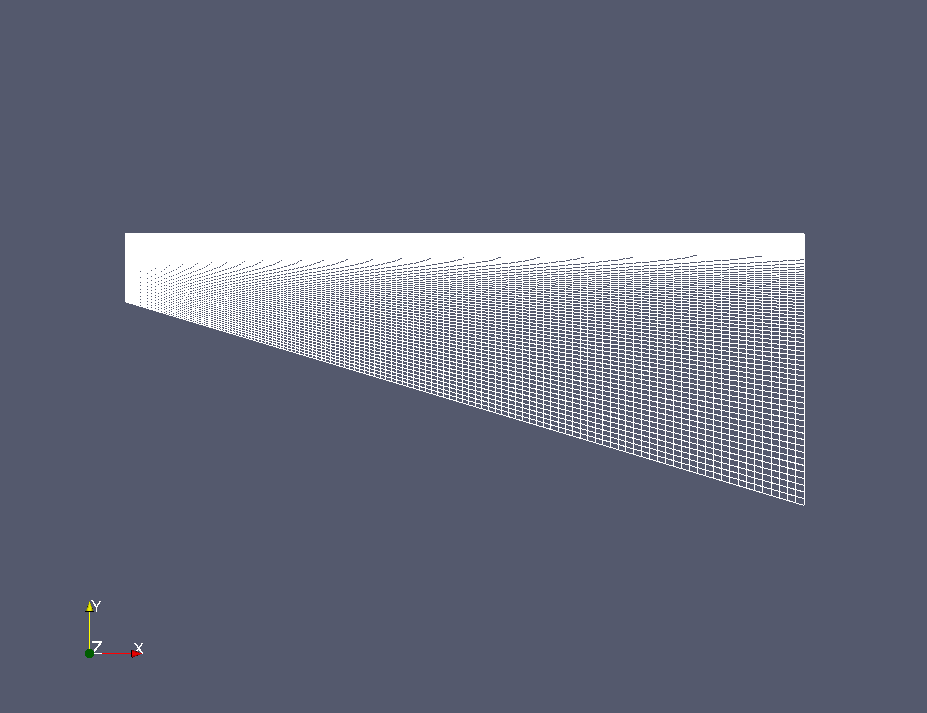
\includegraphics[width=10cm]{./chap2-flat-plate/figs/grid.png}
 \end{center}
 \caption{Computational mesh}
 \label{computational-mesh}
\end{figure}
Three sets of grids were used for this test case - a fine grid
(160$\times$140 cells), a medium grid (80$\times$70 cells), and a coarse (40$\times$35 cells).
The $y^+$ for the grids were lesser than 1.0, except in the first few wall
cells from the leading edge where the boundary layer was establishing.
It was also ensured that there were at least 15 cells within the
boundary layer for most parts of the computational domain.
%-----------------------------------------------------------------
\subsection{Grid convergence}
%\label{}
%
The grid spatial discretisation error can be estimated by using the
Richardson's Extrapolation procedure described in Roache \cite{Roache1998}. Being
the more sensitive parameter to grid refinement, the spatial discretisation
error of the skin friction coefficient is examined, as shown in
Figure~\ref{spatial-discretisation-error}. The value of the errors for all
three grids should follow the equality specified by Roy \& Blottner \cite{Roy2003} if
the mesh levels are sufficiently refined to be in the second-order asymptotic
range. In the turbulent region (beyond $x$ = 0.2\,m), it can be seen that this equality
is satisfied, and that the spatial discretisation errors are below 0.5\% (check).
The high levels of spatial discretisation errors observed in the region between
$x$ = 0.0\,m to $x$ = 0.15\,m are brought about by the transitioning of the boundary layer
and the singularity at the leading edge of the plate. This effect has also been
observed by Roy \& Blottner \cite{Roy2003}. It can be assumed from this study that the solutions
are sufficiently grid-independent.
\begin{figure}[h]
 \begin{center} \vspace{1cm}
  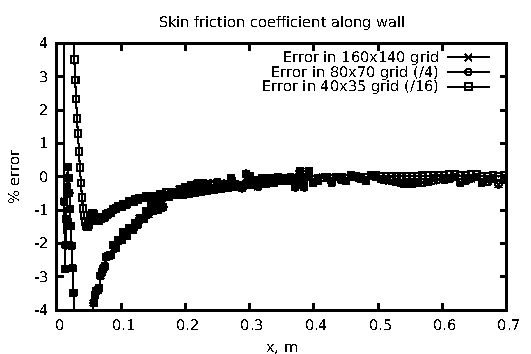
\includegraphics[width=10cm]{./chap2-flat-plate/figs/coles-x05-cf-error.pdf}
 \end{center}
 \caption{Grid convergence check}
 \label{spatial-discretisation-error}
\end{figure}
%\begin{figure}[h]
% \centering
% \subfigure[Caption for first subfigure]{
%   \label{FirstSubFigure}
%   \fbox{Contents of first subfigure}
%   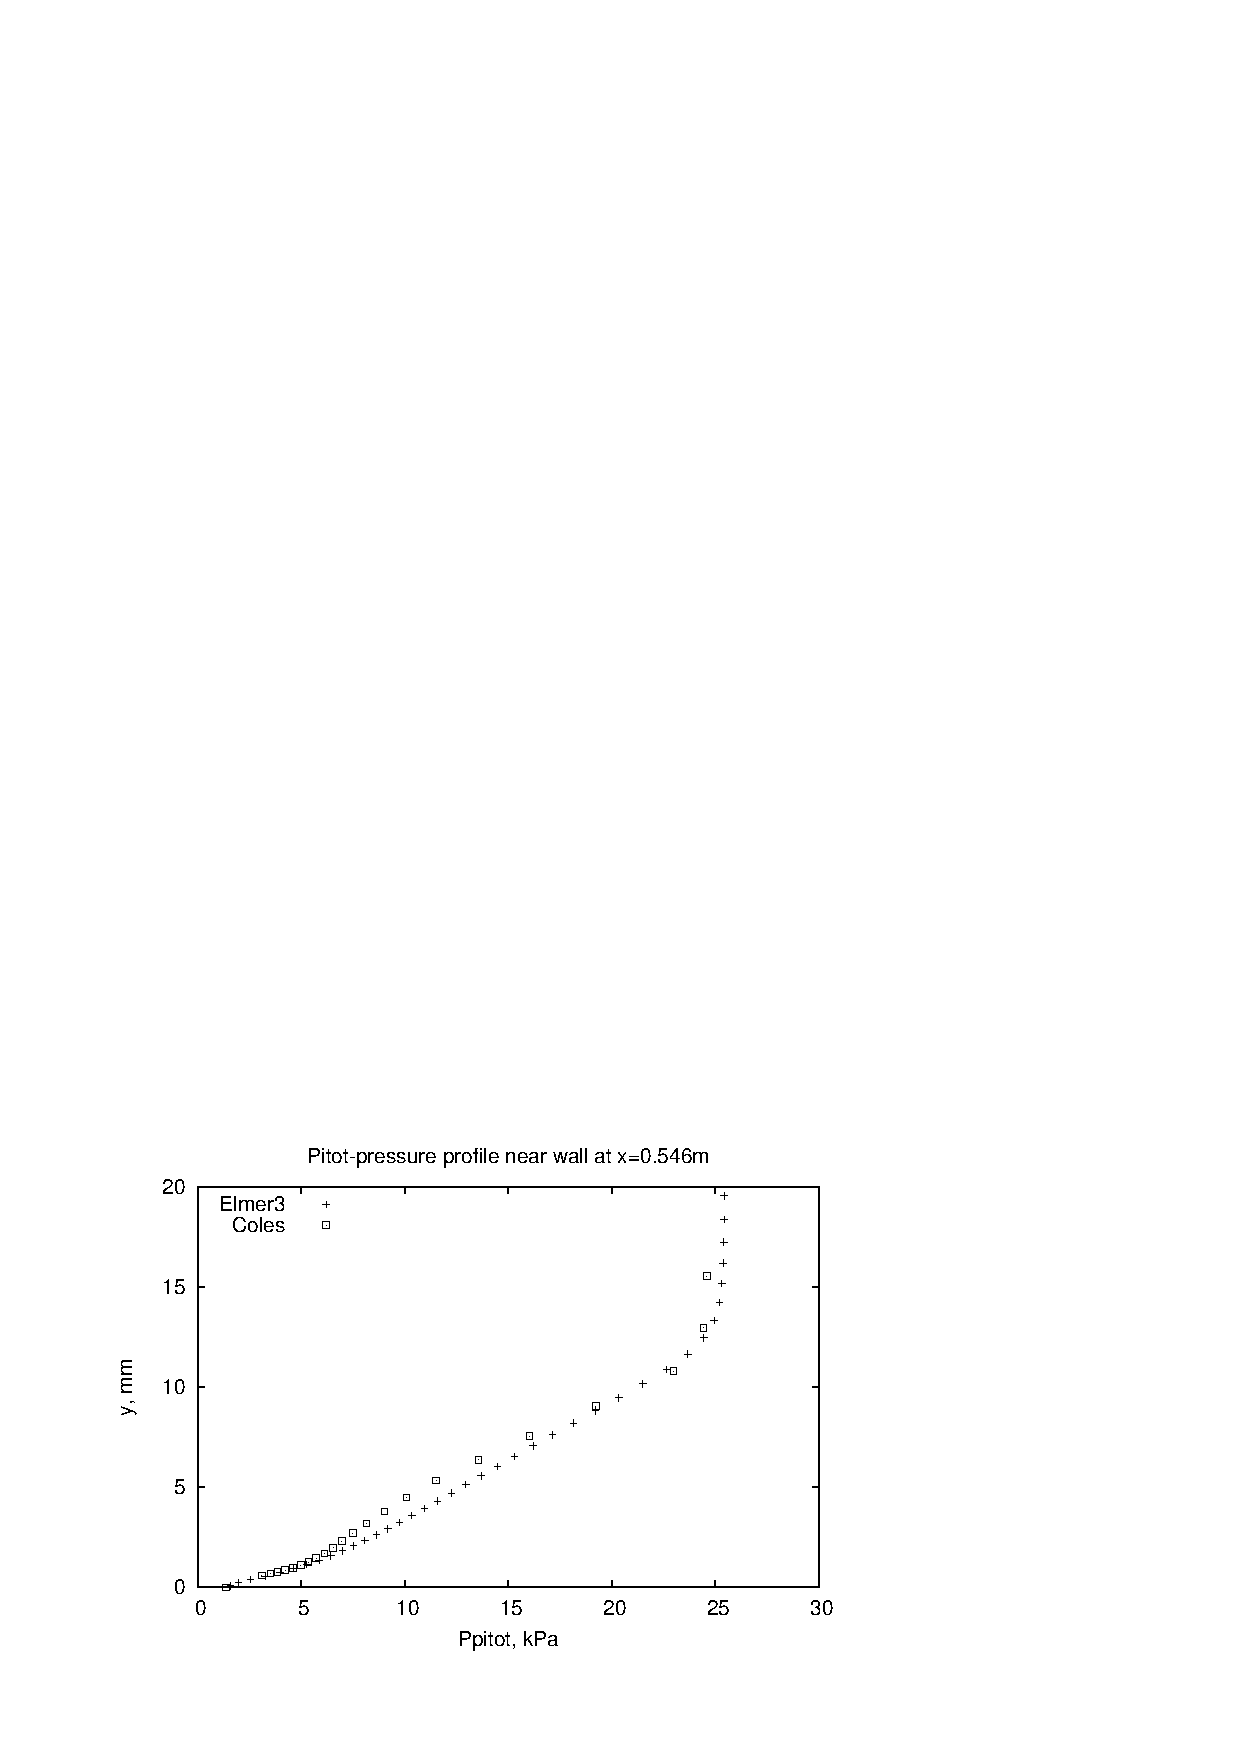
\includegraphics[width=7cm]{./chap2-flat-plate/figs/coles-x05-pitot.png}
% }
% \subfigure[Caption for second subfigure]{
%   \label{SecondSubFigure}
%   \fbox{Contents of second subfigure}
% 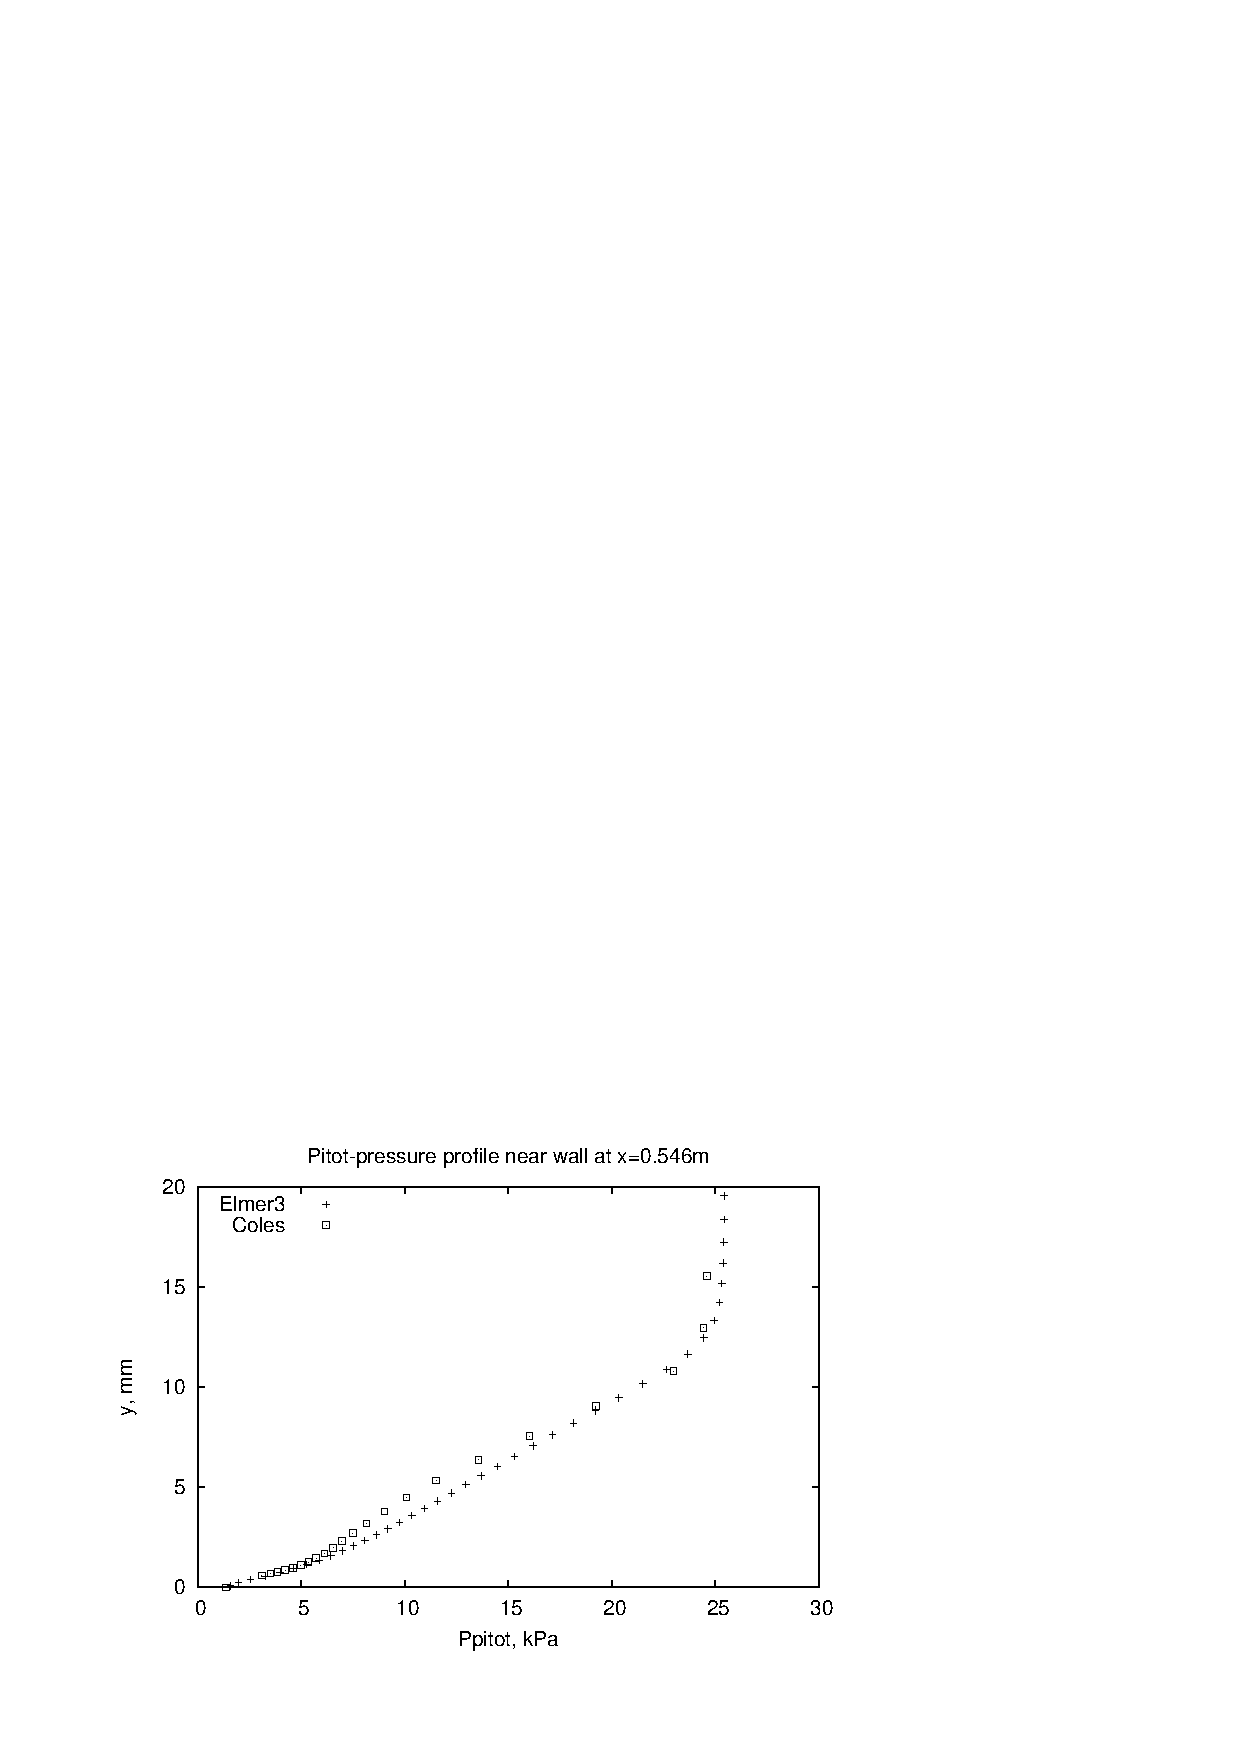
\includegraphics[width=7cm]{./chap2-flat-plate/figs/coles-x05-pitot.png}
% }
% \caption{Caption for the overall figure}
% \label{grid-convergence-fig}
%\end{figure}
%------------------------------------------------------------------
\subsection{Sensitivity to freestream turbulence properties}
\label{flat-plate-sensitivity}
%
The $k$-$\omega$ model has been known to be sensitive to the freestream 
values of turbulence properties. To assess this sensitivity, values of 
freestream turbulence intensity and turbulent-to-laminar viscosity ratio 
have been varied within the recommended range previously discussed in 
Section~\ref{section-intro-recommended-guidelines}. Table~\ref{sensitivity-study-matrix} 
shows a matrix of test cases set up to examine this sensitivity. 
Figures~\ref{flat-plate-BL-profile-546mm} and \ref{flat-plate-cf} show the computed boundary layer profiles
at $x$ = 0.546\,m and the values of skin friction coefficient along the wall respectively for the nine test cases.
The boundary layer profiles and skin friction coefficient values show that the $k$-$\omega$ model 
is indeed sensitive to the values of freestream turbulence properties, with the largest variations
in the pitot pressure and density profiles. The skin friction coefficient plot also reveals that
the boundary layer may be transitioning at different locations for different freestream turbulence properties.
This indicates that the variation in boundary layer profiles for the nine cases 
in Figures ~\ref{flat-plate-BL-profile-546mm} 
and \ref{flat-plate-cf} could also be partially brought about by the difference
in the boundary layer transitioning location. The effect of the $k$-$\omega$ model's sensitivity to freestream 
turbulence properties will be further discussed during the comparison of the numerical and experimental results
in Section~\ref{flat-plate-results-and-discussions}.
\begin{table}[h]
  \caption{Test matrix for the study of turbulence model sensitivities}
  \label{sensitivity-study-matrix}
  \begin{center}
    \begin{tabular}{ccccl}
      \hline\hline
      & \multicolumn{3}{c}{Turbulence Intensity} \\
      \hline
      $\mu_t/\mu$ & 1.0\%  & 5.0\%  & 10.0\% \\
      \hline
      1.0     &  Case 1    &  Case 4    &  Case 7   \\
      10.0    &  Case 2    &  Case 5    &  Case 8   \\
      100.0   &  Case 3    &  Case 6    &  Case 9   \\
      \hline \hline
    \end{tabular}
  \end{center}
\end{table}
%
\begin{figure}[h]
 \centering
 \subfigure[Pitot pressure]{
   \label{flat-plate-pitot}
%   \fbox{Contents of first subfigure}
   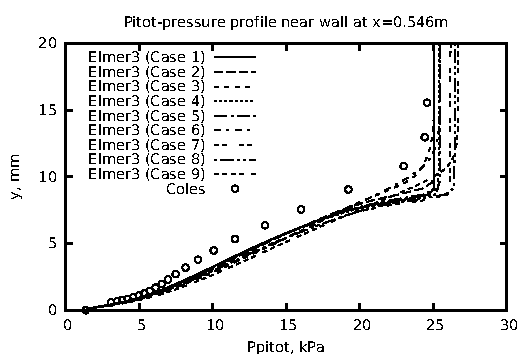
\includegraphics[width=7cm]{./chap2-flat-plate/figs/coles-x-546-pitot.pdf}
 }
 \subfigure[Density]{
   \label{flat-plate-density}
%   \fbox{Contents of second subfigure}
 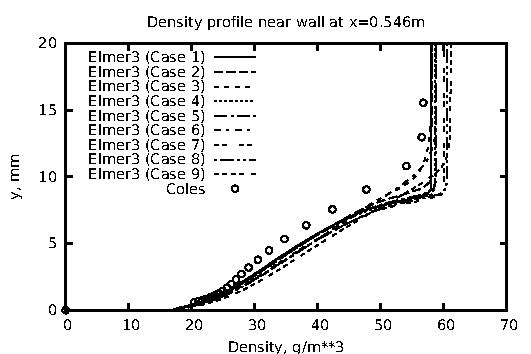
\includegraphics[width=7cm]{./chap2-flat-plate/figs/coles-x-546-density.pdf}
 }
 \subfigure[Temperature]{
   \label{flat-plate-temperature}
%   \fbox{Contents of first subfigure}
   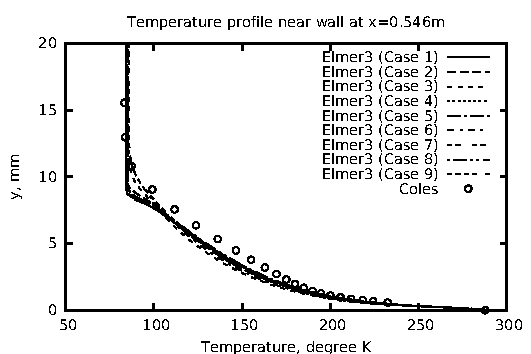
\includegraphics[width=7cm]{./chap2-flat-plate/figs/coles-x-546-temperature.pdf}
 }
 \subfigure[$u$-velocity]{
   \label{flat-plate-u-velocity}
%   \fbox{Contents of second subfigure}
 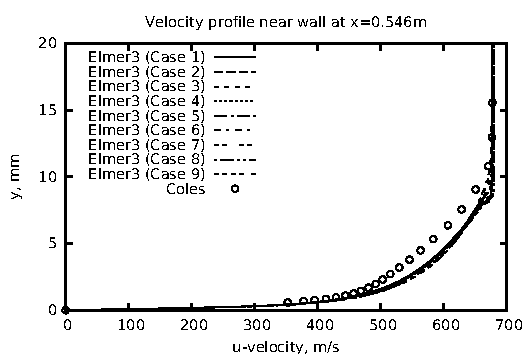
\includegraphics[width=7cm]{./chap2-flat-plate/figs/coles-x-546-u.pdf}
 }
 \caption{Near-wall boundary layer profiles at $x$ = 0.546\,m}
 \label{flat-plate-BL-profile-546mm}
\end{figure}
%
\begin{figure}[h]
 \begin{center}
  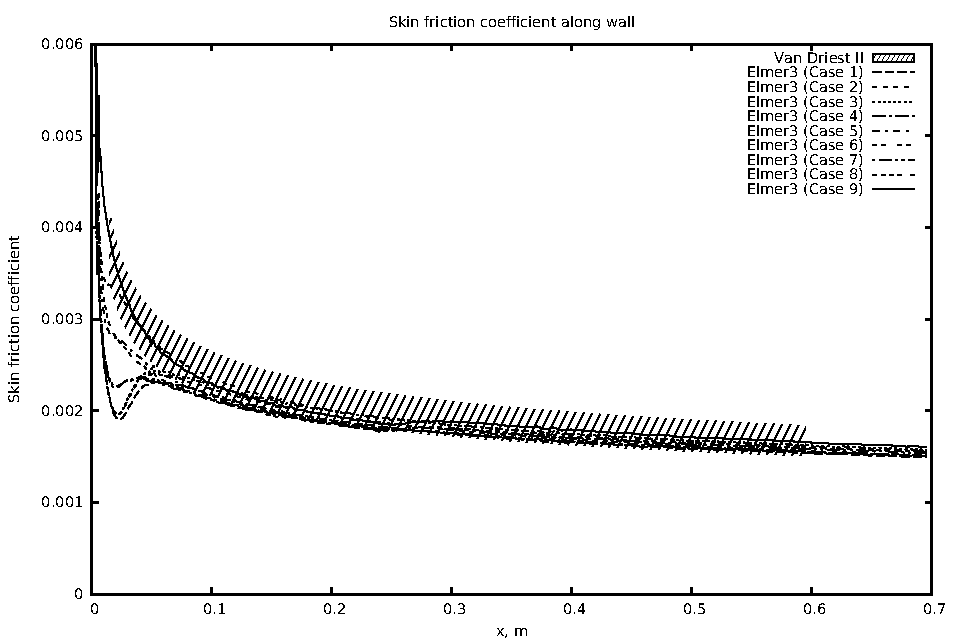
\includegraphics[width=12.5cm]{./chap2-flat-plate/figs/coles-x-cf.pdf}
 \end{center}
 \caption{Skin friction coefficient along flat plate}
 \label{flat-plate-cf}
\end{figure}

%------------------------------------------------------------------
\subsection{Results \& discussions}
\label{flat-plate-results-and-discussions}
%
Figures~\ref{flat-plate-BL-profile-546mm} and \ref{flat-plate-BL-profile-646mm} 
show the comparison between the experimental and numerical boundary layer 
profiles at $x$ = 0.546\,m and $x$ = 0.646\,m respectively. It can be seen that 
the profiles at $x$ = 0.646\,m match the experimental data better than those at 
$x$ = 0.546\,m, even though the experimental profiles were sampled at $x$ = 0.546\,m.
There is a certain level of uncertainty regarding the way the boundary layer transitions with
the boundary layer trip used in the experiments. In addition, this method of tripping the
boundary layer may not be accurately modelled by the turbulence model. The use of 
non-dimensionalised flow variables should somewhat alleviate this issue. 
Figure~\ref{flat-plate-dimensionless-velocity} shows the non-dimensionalised 
velocity against the non-dimensionalised distance from the wall. It can be
seen that the dimensionless velocity profiles at both locations match each other, and also the
incompressible logarithmic law-of-the-wall velocity profile.
%
\begin{figure}[h]
 \centering
 \subfigure[Pitot pressure]{
   \label{flat-plate-pitot}
%   \fbox{Contents of first subfigure}
   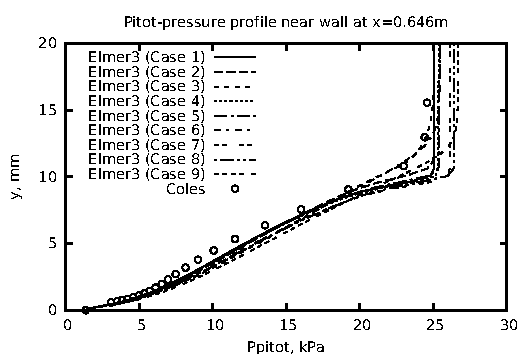
\includegraphics[width=7cm]{./chap2-flat-plate/figs/coles-x-646-pitot.pdf}
 }
 \subfigure[Density]{
   \label{flat-plate-density}
%   \fbox{Contents of second subfigure}
 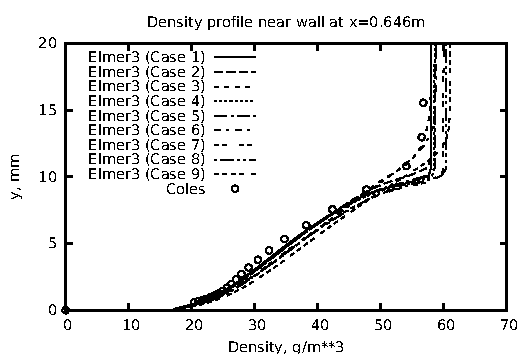
\includegraphics[width=7cm]{./chap2-flat-plate/figs/coles-x-646-density.pdf}
 }
 \subfigure[Temperature]{
   \label{flat-plate-temperature}
%   \fbox{Contents of first subfigure}
   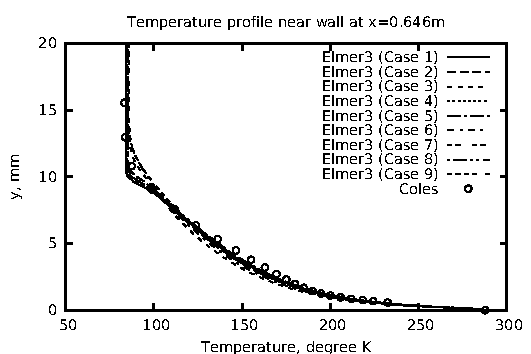
\includegraphics[width=7cm]{./chap2-flat-plate/figs/coles-x-646-temperature.pdf}
 }
 \subfigure[$u$-velocity]{
   \label{flat-plate-u-velocity}
%   \fbox{Contents of second subfigure}
 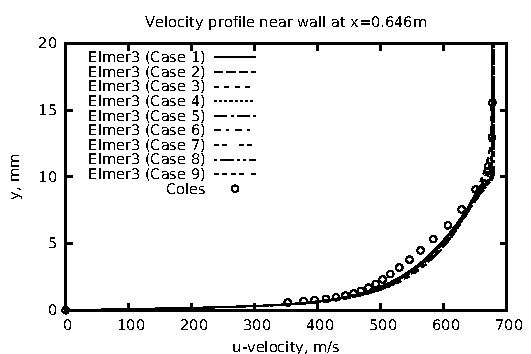
\includegraphics[width=7cm]{./chap2-flat-plate/figs/coles-x-646-u.pdf}
 }
 \caption{Near-wall boundary layer profiles at $x$ = 0.646\,m}
 \label{flat-plate-BL-profile-646mm}
\end{figure}
%
\begin{figure}[h]
 \begin{center}
  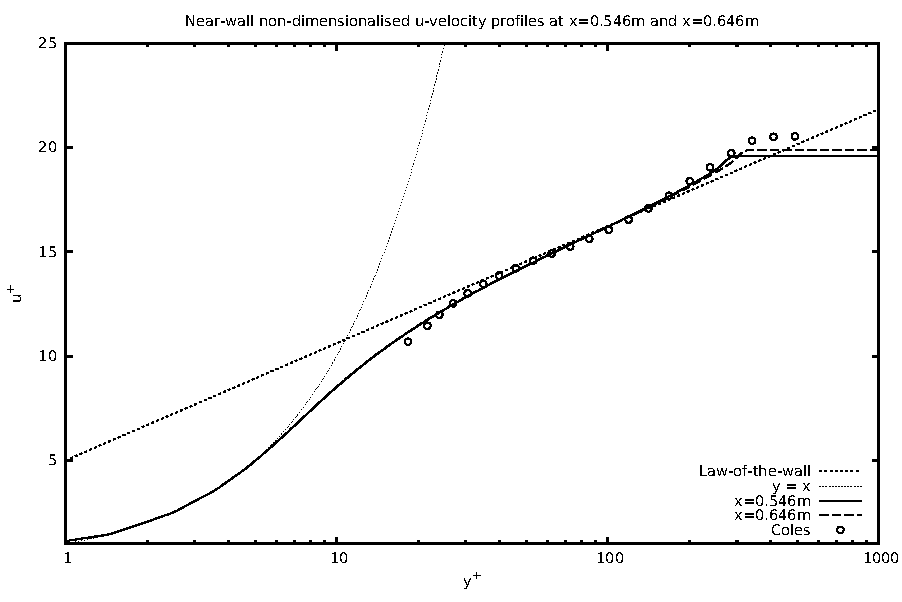
\includegraphics[width=12.5cm]{./chap2-flat-plate/figs/coles-x-dimensionless.pdf}
 \end{center}
 \caption{Non-dimensionalised velocity profiles}
 \label{flat-plate-dimensionless-velocity}
\end{figure}
%
Figure~\ref{flat-plate-cf} shows a comparison between the skin friction coefficient 
computed using van Driest's turbulent skin friction theory and computed using Eilmer3. 
Using an uncertainty band of $\pm$10\% for the theoretical plot, it can be seen that 
the numerical results are within the uncertainty band of van Driest's turbulent skin 
friction theory. This shows that the $k$-$\omega$ model in Eilmer3 can be used to 
predict turbulent skin friction coefficient on a flat plate, despite the model's 
sensitivity to freestream turbulence properties.
%------------------------------------------------------------------

% mallinson-cylinder.tex
%
\newpage
\section{Mallinson's hollow cylinder}
\label{chapter-cylinder}
%
The second validation test case is that of a Mach 8.8 flow 
over a hollow cylinder. This test case is basically an axisymmetric
analogy of the flat plate test case examined in Chapter~\ref{chapter-flat-plate}. 
It serves as an excellent exercise to test the axisymmetric turbulence 
terms in the $k$-$\omega$ model. The large experimental data set of surface 
pressure and heat flux provided in Mallinson et. al. \cite{Mallinson2000} 
and in Boyce \& Hillier \cite{Boyce2000} is compared with predictions from 
Eilmer3 simulations. This exercise also explores the $k$-$\omega$ model's
sensitivity to $y+$ values and maximum cell aspect ratios.

%------------------------------------------------------------------
\subsection{Details of flow problem}
%\label{}
%
The experimental setup used by Mallinson et al. is shown 
schematically in Figure~\ref{figure-cylinder-exp-setup}.
%
\begin{figure}[htbp]
\begin{center}
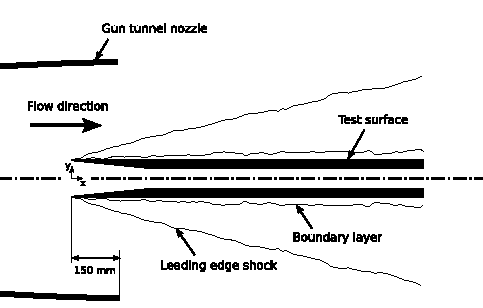
\includegraphics[width=13cm]{./chap3-mallinson-cylinder/figs/experimental-setup.pdf}
\end{center}
\caption{Schematic diagram of the experimental setup for the hollow 
         cylinder test case}
\label{figure-cylinder-exp-setup}
\end{figure}
%
A turbulent boundary layer was allowed to grow on a hollow sharp-nosed 
cylindrical centrebody that had been aligned with a hypersonic flow 
produced by the Imperial College Gun Tunnel. This boundary layer was 
allowed to transition naturally to turbulence from its laminar 
state. Since the test surface was the external surface of the cylinder, 
this test case had the advantage that the body surface was offset from 
the tunnel axis, hence avoiding any centreline focusing effects. The
cylinder was 850 mm long and had an outer diameter of 75 mm. The leading
edge of this cylinder was positioned 150 mm upstream of the nozzle exit
plane for these experiments.

An extensive calibration of the nozzle outflow was conducted by 
Mallinson et. al. to provide as precise a specification of 
freestream flow conditions as possible. Using the static pressure
measured on the surface of the hollow cylinder together with
the reservoir static pressure, freestream pitot pressure 
and stagnation point heat flux, the Mach number was inferred.
The inferred Mach number with axial and radial static pressure 
distributions were then used for a Method-of-Characteristics (MOC) 
calculation to determine the flow conditions at the leading edge
of the hollow cylinder.

The MOC calculations revealed that the nozzle outflow was not exactly 
uniform; the outflow was somewhat radial. The outflow diverged from the
axis of the nozzle by about 0.005$^{\circ}$ per millimetre. As the 
outflow was radial, there was also an axial gradient, $\delta M /\delta x$, 
of about 0.24 per metre. Nominal conditions at the leading edge of the 
cylinder are shown in Table~\ref{inflow-conditions-cylinder}. 
%
\begin{table}[h]
  \caption{Nominal inflow conditions for hollow cylinder test case}
  \label{inflow-conditions-cylinder}
  \begin{center}
    \begin{tabular}{cccl}
      \hline\hline
      Parameter & Value   & Units \\
      \hline
      Test gas    & Nitrogen &    \\
      $M_{\infty,nominal}$  & 8.8      &     \\
      $p_{\infty,nominal}$  & 3.3e3    & Pa  \\
      $T_{\infty,nominal}$  & 69.7     & K   \\
      $u_{\infty,nominal}$  & 1498.0   & m/s \\
      \hline \hline
    \end{tabular}
  \end{center}
\end{table}
%
Static pressure distributions on the cylinder surface were measured 
using Kulite XCS-093 pressure transducers. Wall surface temperature 
time histories measured using platinum/MACOR thin film gauges were 
used together with Schultz \& Jones' theory \cite{Schultz1973} to infer the 
values of surface heat flux. The pressure transducers and thin film 
gauges were located in axial arrays at 120$^{\circ}$ pitch around 
the outside circumference of the hollow model. Uncertainties in the 
static pressure and heat flux measurements were estimated to be 
$\pm$4\% and $\pm$5\% respectively. Experimentally measured values 
of static pressure and heat flux along the cylinder wall are used 
for comparison with results from Eilmer3 simulations. 


%------------------------------------------------------------------
\subsection{Details of computational approach}
%\label{}
%
The setup of the mesh for this test case is similar to that
previously used in the flat plate test case in Chapter~\ref{chapter-flat-plate}.
While the test case in Chapter~\ref{chapter-flat-plate} was aimed at
showing the $k$-$\omega$ model's sensitivity to freestream turbulence
properties, this test case aims to investigate the $k$-$\omega$ model's 
sensitivity to differing grids. Two main aspects of grid configurations
are examined in this chapter - $y^+$ and cell aspect ratio.
\begin{figure}[h]
\begin{center}
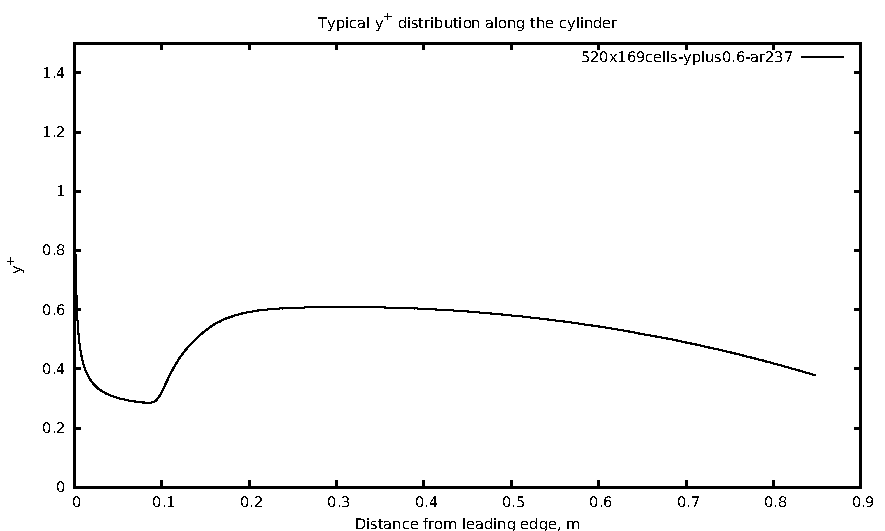
\includegraphics[width=15cm]{./chap3-mallinson-cylinder/figs/typical-yplus-distribution.pdf}
\end{center}
\caption{Typical $y^+$ distribution along the test surface}
\label{figure-cylinder-typical-yplus-dist}
\end{figure}
%
\begin{table}[h]
  \caption{Different grids used for the hollow cylinder test case}
  \label{table-cylinder-grids}
  \begin{center}
    \begin{tabular}{cccccl}
      \hline\hline
      Grid & Number       & Number       & $y^+$ & Maximum \\
           & of $x$-cells & of $y$-cells &       & aspect ratio \\
      \hline
      100x33cells-yplus3.0-ar215   & 100  &  33 & 3.0 & 215 \\
      200x65cells-yplus1.5-ar227   & 200  &  65 & 1.5 & 227 \\
      200x65cells-yplus0.4-ar922   & 200  &  65 & 0.4 & 922 \\
      400x130cells-yplus0.8-ar235  & 400  & 130 & 0.8 & 235 \\
      400x130cells-yplus1.7-ar114  & 400  & 130 & 1.7 &  92 \\
      400x130cells-yplus0.2-ar961  & 400  & 130 & 0.2 & 961 \\
      400x130cells-yplus0.2-ar864  & 400  & 130 & 0.2 & 864 \\
      600x130cells-yplus0.2-ar577  & 600  & 130 & 0.2 & 577 \\
      520x169cells-yplus0.6-ar237  & 520  & 169 & 0.6 & 237 \\
      \hline \hline
    \end{tabular}
  \end{center}
\end{table}
%
\begin{figure}[h]
 \begin{center}
  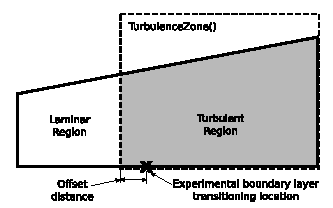
\includegraphics[width=10cm]{./chap3-mallinson-cylinder/figs/turbulence-zone.pdf}
 \end{center}
 \caption{Offset distance to estimate the start of the \texttt{TurbulenceZone()}}
 \label{figure-cylinder-turbulence-zone}
\end{figure}


Table~\ref{table-cylinder-grids} shows the different grids that were used.
Note that the $y^+$ specified in the fourth column of Table~\ref{table-cylinder-grids}
is only an averaged $y^+$ value taken between $x$ = 0.2 m and $x$ = 0.8 m
- a typical $y^+$ distribution along the test surface is shown in 
Figure~\ref{figure-cylinder-typical-yplus-dist}.

The test gas used was nitrogen with an ideal gas assumption, a 
constant specific heats ratio of 1.4 and a gas constant of 296.8 J/kg.K. 
An isothermal wall at a temperature of 295 K was used. 
The setup of the supersonic inflow boundary condition is different
to the flat plate test case due to the presence of flow angularity
in the inflow. This angularity was taken into account by using the 
user-defined boundary condition \texttt{UserDefinedBC("")} 
available in Eilmer3. An example showing the usage of \texttt{UserDefinedBC("")}
can be found in the Eilmer3 user guide. For this test case,
this boundary condition was specified by adding  \texttt{UserDefinedBC("udf-supersonic-in.lua")} 
in the \textit{Python} setup script. The \texttt{udf-supersonic-in.lua} file 
is shown in Section~\ref{section-udf-supersonic-in-lua}.

The $k$-$\omega$ model has always been known to predict premature
transitioning for boundary layers \cite{Wilcox2006}. To counteract this 
and simulate boundary layer transitioning, an initial simulation was
performed to estimate the transition location predicted by the 
$k$-$\omega$ model. This distance is then used as an offset distance 
to define the start of the turbulent block, as shown in 
Figure~\ref{figure-cylinder-turbulence-zone}.

% Might configure Eilmer3 to use Dan's in-code "heat flux extractor"..
%While surface static pressure can be directly extracted from the 
%simulations, surface heat flux has to be inferred using the 
%temperatures in the first cells along the wall. The heat flux can
%then be computed by ..... blah blah ..

%------------------------------------------------------------------
%\subsection{Grid convergence}
%\label{}
%

%------------------------------------------------------------------
\subsection{Results \& discussion}
%\label{}
%
Figures~\ref{cylinder-bl-profiles}, \ref{cylinder-surface-static-pressure-compare-grid} 
and \ref{cylinder-surface-heat-flux-compare-grid} show the numerical results for 
four different grid resolutions. In contrast to the boundary layer profiles shown 
in Figure~\ref{cylinder-bl-profiles}, the simulated wall static pressure and heat 
flux distribution in Figures~\ref{cylinder-surface-static-pressure-compare-grid} and 
\ref{cylinder-surface-heat-flux-compare-grid} 
do not appear to show any form of grid convergence. Since the wall static pressure 
and heat flux distribution are values taken from the first cells off the wall, this 
indicates that the overall influence on the external flowfield from the wall cells is 
not too significant. If grid convergence was considered based only on the boundary 
layer profiles, the fine grid would have been considered to produce sufficiently 
grid-converged results.
%
\begin{figure}[h]
 \begin{center}
  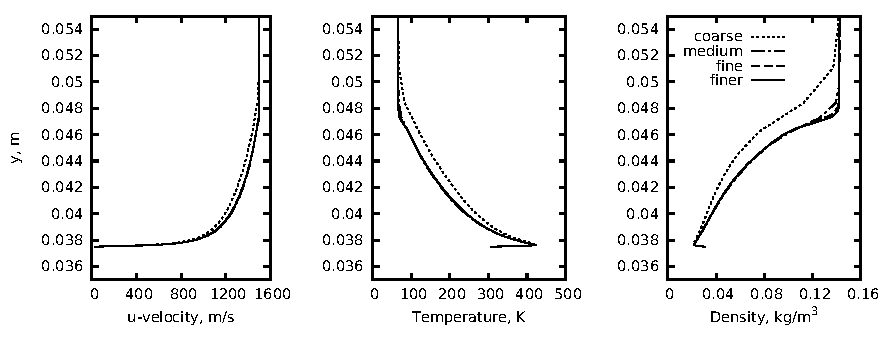
\includegraphics[width=15cm]{./chap3-mallinson-cylinder/figs/boundary-layer-profile-800mm.pdf}
 \end{center}
 \caption{Near wall boundary layer profiles at $x$ = 0.8 m 
          (where ``coarse" is the ``100x33cells-yplus3.0-ar215" grid, 
          ``medium" is the ``200x65cells-yplus1.5-ar227" grid,
          ``fine" is the ``400x130cells-yplus0.8-ar235" grid, and
          ``finer" is the ``520x169cells-yplus0.6-ar237" grid.)}
 \label{cylinder-bl-profiles}
\end{figure}
\begin{figure}[h]
 \begin{center}
  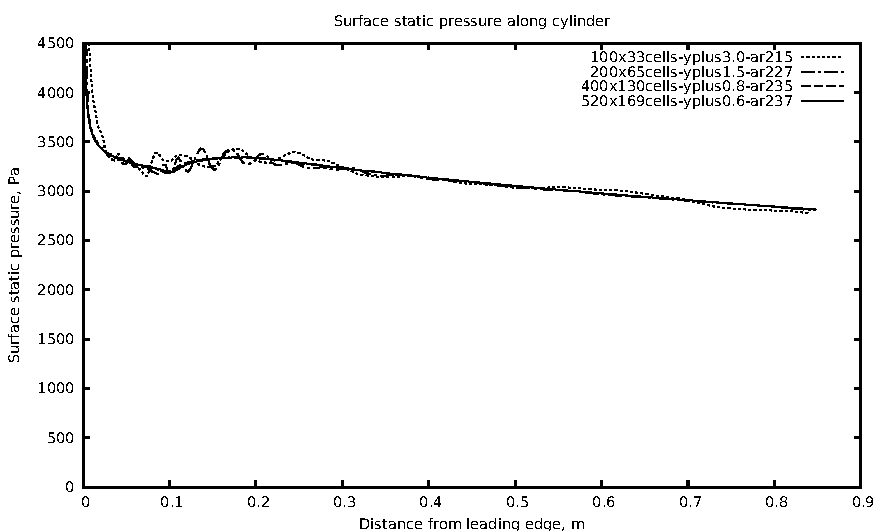
\includegraphics[width=15cm]{./chap3-mallinson-cylinder/figs/compare-grid-resolution-pressure.pdf}
 \end{center}
 \caption{Surface static pressure distribution for different grid resolutions}
 \label{cylinder-surface-static-pressure-compare-grid}
%\end{figure}
%\begin{figure}[h]
\vspace{2cm}
 \begin{center}
  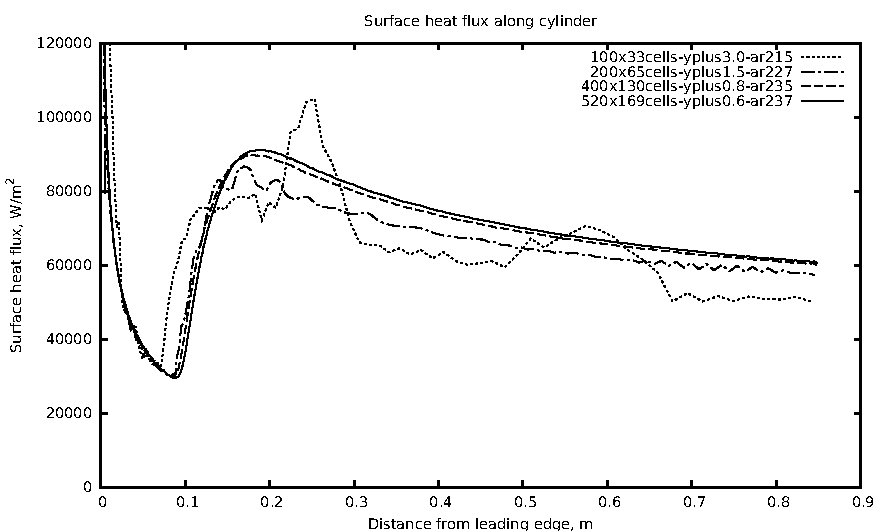
\includegraphics[width=15cm]{./chap3-mallinson-cylinder/figs/compare-grid-resolution-heat-flux.pdf}
 \end{center}
 \caption{Surface heat flux distribution for different grid resolutions}
 \label{cylinder-surface-heat-flux-compare-grid}
\end{figure}

The fluctuations in the static pressure and heat flux, and the non-converging heat 
flux values evident in Figures~\ref{cylinder-surface-static-pressure-compare-grid} and 
\ref{cylinder-surface-heat-flux-compare-grid} are likely to be due to the differences in 
the $y^+$ values for each grid. As the grid is refined, the $y^+$ value decreases.
Figures~\ref{cylinder-surface-static-pressure-compare-grid} and \ref{cylinder-surface-heat-flux-compare-grid} 
show that the fluctuations in the wall static pressure and heat flux values are not present for 
grids with $y^+$ values lesser than 1.0 - the minimum $y^+$ value recommended earlier 
in Chapter~\ref{chapter-flat-plate}. To closer examine the influence of $y^+$ on the 
simulations, the grid clustering for the ``400x130cells-yplus0.8-ar235" grid is 
adjusted to vary the $y^+$ values. The simulated wall static pressure and heat flux 
distributions are shown in Figures~\ref{cylinder-surface-static-pressure-compare-yplus}
and \ref{cylinder-surface-heat-flux-compare-yplus} respectively.
%
\begin{figure}[h]
 \begin{center}
  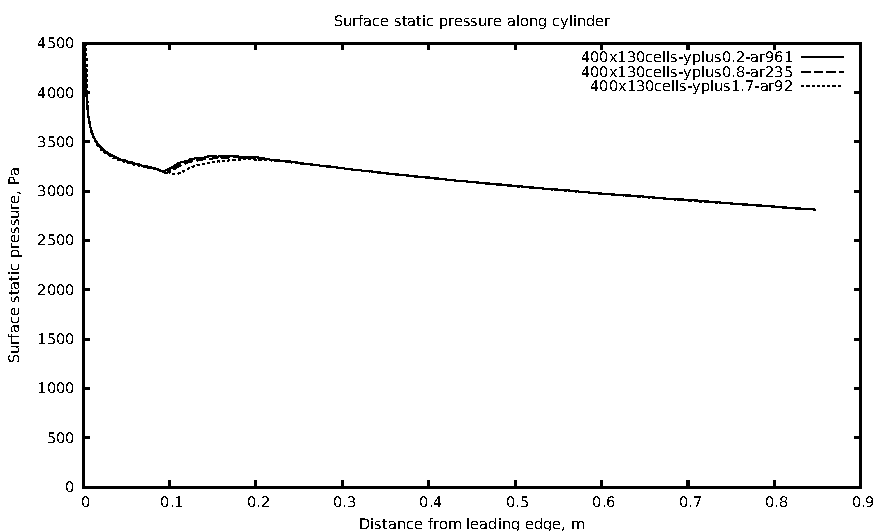
\includegraphics[width=15cm]{./chap3-mallinson-cylinder/figs/compare-yplus-pressure.pdf}
 \end{center}
 \caption{Surface static pressure distribution for grids with different $y^+$ values}
 \label{cylinder-surface-static-pressure-compare-yplus}
%\end{figure}
%\begin{figure}[h]
\vspace{2cm}
 \begin{center}
  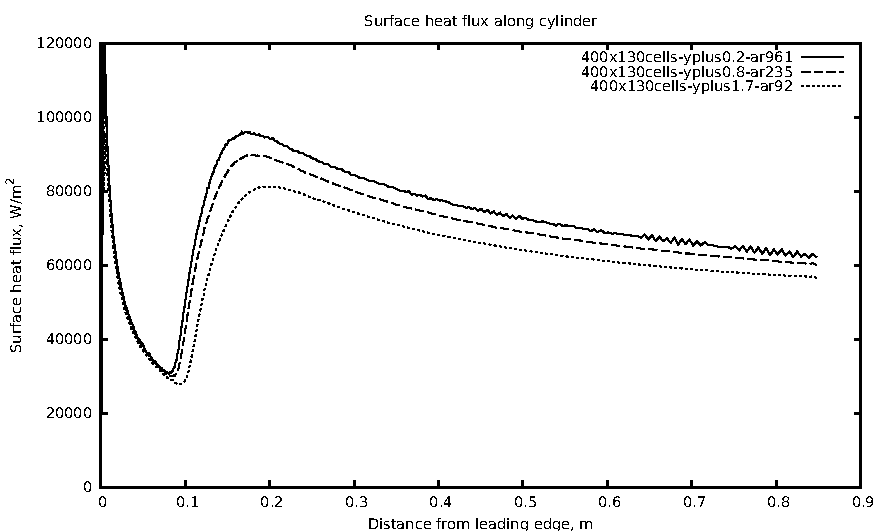
\includegraphics[width=15cm]{./chap3-mallinson-cylinder/figs/compare-yplus-heat-flux.pdf}
 \end{center}
 \caption{Surface heat flux distribution for grids with different $y^+$ values}
 \label{cylinder-surface-heat-flux-compare-yplus}
\end{figure}

It can be observed that only the heat flux distribution is truly sensitive to the 
differences in $y^+$; the average values of pressure distribution are similar for 
all three grids. To quantify the $k$-$\omega$ model's sensitivity to $y^+$ values, the 
$y^+$ value is plotted against the wall heat flux value at an arbitrary location 
($x$ = 0.8 m) for each grid in Figure~\ref{cylinder-surface-heat-flux-compare-yplus},
and shown in Figure~\ref{cylinder-compare-surface-heat-flux-for-different-yplus}. 
A line fitted through these points is extrapolated to estimate the wall heat flux value 
if an infinitesimally small $y^+$ is used. A comparison between this extrapolated 
wall heat flux value to that for $y^+$ = 0.2 gives a difference of approximately 
1\%. For a $y^+$ of 0.8, the difference is about 6\% and for a $y^+$ of 1.7, this
difference is about 13\%. For this test case, where the experimental uncertainties 
are about $\pm$5\%, the use of the numerical results from grids with  a $y^+$ 
lesser than 0.8 is acceptable.
%
\begin{figure}[h]
 \begin{center}
  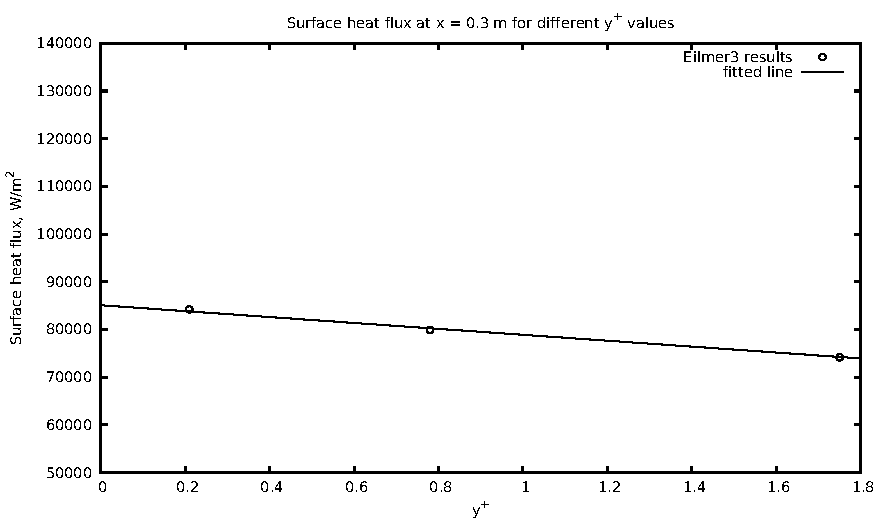
\includegraphics[width=15cm]{./chap3-mallinson-cylinder/figs/yplus-sensitivity.pdf}
 \end{center}
 \caption{Surface heat flux values at $x$ = 0.8 m for different $y^+$ values}
 \label{cylinder-compare-surface-heat-flux-for-different-yplus}
\vspace{2cm}
\end{figure}

It can also be noted in Figure~\ref{cylinder-surface-heat-flux-compare-yplus} that 
the surface heat flux distribution for the ``400x130cells-yplus0.2-ar961" grid 
become unstable downstream of $x$ = 0.3 m. This instability is brought about by 
the aspect ratio of the cells. Clustering to the surface to achieve low
$y^+$ values tends to lead to cells with high aspect ratios. To quantify the
effects of cell aspect ratio on the simulations, results from grids with different
cell aspect ratios are plotted in Figure~\ref{cylinder-surface-heat-flux-compare-aspect-ratio}.
The grids with a maximum cell aspect ratio of around 200 seem stable. When the 
maximum cell aspect ratio is around 577, small instabilities start appearing. For
grids with maximum cell aspect ratio higher than 600, significant instabilities
can be seen in the surface heat flux traces. It is therefore recommended that
maximum cell aspect ratios be kept below 600 for all simulations. Since this
recommendation is deduced from a test case which has a relatively simple flow,
it is highly possible that a smaller aspect ratio is needed in regions with 
stronger flow gradients or flow separation.
%
\begin{figure}[h]
 \begin{center}
  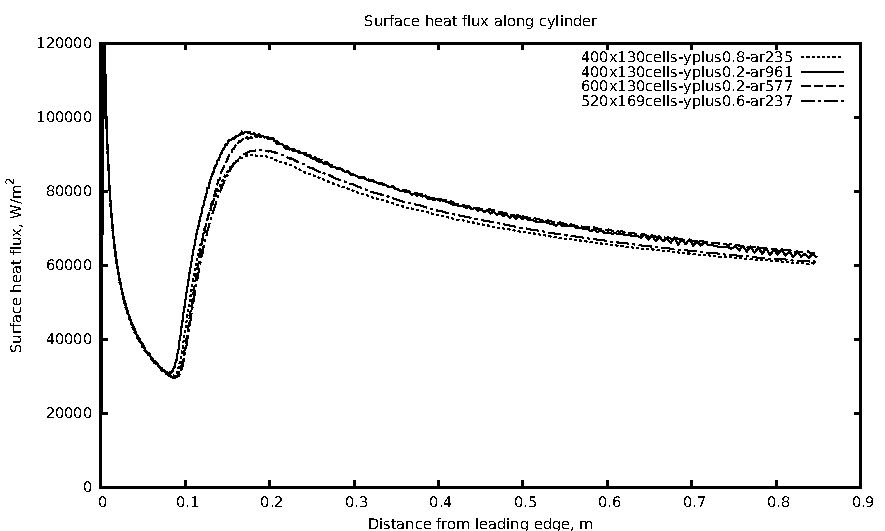
\includegraphics[width=15cm]{./chap3-mallinson-cylinder/figs/compare-aspect-ratio-heat-flux.pdf}
 \end{center}
 \caption{Surface heat flux distribution for grids with different maximum cell aspect ratio}
 \label{cylinder-surface-heat-flux-compare-aspect-ratio}
\end{figure}

Among the nine grids listed in Table~\ref{table-cylinder-grids}, the 
``600x130cells-yplus0.2-ar577" grid is taken to be the most suitable
one for comparison with the experimental data - it is sufficiently 
grid-converged for both boundary layer profiles and surface pressure 
and heat flux distributions, it has a maximum aspect ratio of less
than 600, and it has an average $y^+$ of about 0.2. The numerical results
for this grid are plotted against the experimental data in 
Figures~\ref{cylinder-surface-static-pressure} and \ref{cylinder-surface-heat-flux}.
The computed surface static pressures agree well with those measured experimentally. 
The slight dip in the surface static pressure distribution at $x$ $\approx$ 0.1 m 
in Figure~\ref{cylinder-surface-static-pressure} is an artefact of the 
turbulence model transitioning the boundary layer from a laminar to a turbulent 
state. 

The surface heat flux distribution in Figure~\ref{cylinder-surface-heat-flux}
can be divided into three regions - laminar region between $x$ $\approx$ 0.0 m 
and 0.1 m, transitioning region between $x$ $\approx$ 0.1 m and 0.16 m, and
turbulent region from $x$ $\approx$ 0.16 m onwards. The laminar surface heat 
flux distribution is well predicted by Eilmer3. The transitioning region also
appears to be well modelled by the $k$-$\omega$ model in Eilmer3. An interesting 
point to note here is that even though the only variable fixed by the user in 
this simulation is the transitioning location, the overall transitioning process 
(the peak, slope and length of surface heat flux distribution in the transitioning 
region) is predicted quite well by the $k$-$\omega$ model. For the turbulent
region, the simulated surface heat flux distribution from $x$ $\approx$ 0.16 m to
$x$ $\approx$ 0.5 m matches the experimental data. However, the numerically 
predicted heat flux deviates progressively from the experimental values downstream 
of $x$ $\approx$ 0.5 m.
%
\begin{figure}[h]
 \begin{center}
  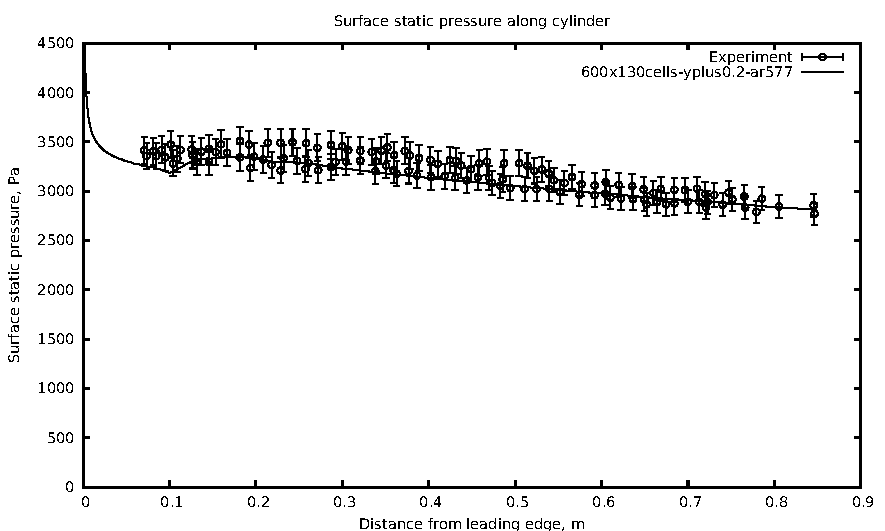
\includegraphics[width=15cm]{./chap3-mallinson-cylinder/figs/final-pressure.pdf}
 \end{center}
 \caption{Surface static pressure distribution}
 \label{cylinder-surface-static-pressure}
%\end{figure}
%\begin{figure}[h]
\vspace{2cm}
 \begin{center}
  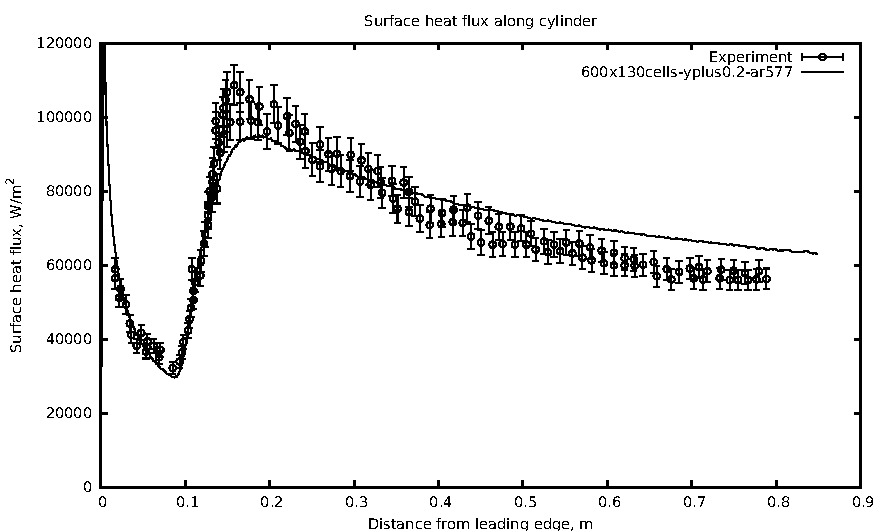
\includegraphics[width=15cm]{./chap3-mallinson-cylinder/figs/final-heat-flux.pdf}
 \end{center}
 \caption{Surface heat flux distribution}
 \label{cylinder-surface-heat-flux}
\end{figure}

In summary, this validation exercise shows that Eilmer3 can be used to predict the
development of an axisymmetric flow on a cylinder. It also shows that the simulated
surface heat flux distribution is more sensitive to the geometrical properties of
the first wall cell (distance from cell centre to wall and cell aspect ratio) than 
the surface pressure distribution. In addition, this exercise also demonstrates that
$y^+$ values and maximum cell aspect ratios should be kept below 1 and 600 respectively. 
The validation of this test case can be extended to test the $k$-$\omega$ model's 
capability in predicted shock-induced separation of an axisymmetric boundary layer. 
Experimental data for the shock-induced separation extension to this test case can be 
found in Boyce \& Hillier \cite{Boyce2000}.

\subsection{udf-supersonic-in.lua}
\label{section-udf-supersonic-in-lua}
\topbar
\lstinputlisting[language={}]{./chap3-mallinson-cylinder/udf-supersonic-in.lua}
\bottombar

% backward-facing-step.tex
%
\newpage
\section{Backward facing step}
%
The third validation test case is that of a Mach 2.0 flow over a
two-dimensional backward-facing step. Experimental data from Eklund et. al. \cite{Eklund1995}
and McDaniel et. al. \cite{McDaniel1991} are  used for this exercise.

%------------------------------------------------------------------
\subsection{Details of flow problem}
%\label{}
%
The experimental setup used by Eklund et. al. is shown 
schematically in Figure~\ref{backward-facing-step-exp-setup-fig}.
%
\begin{figure}[htbp]
\begin{center}
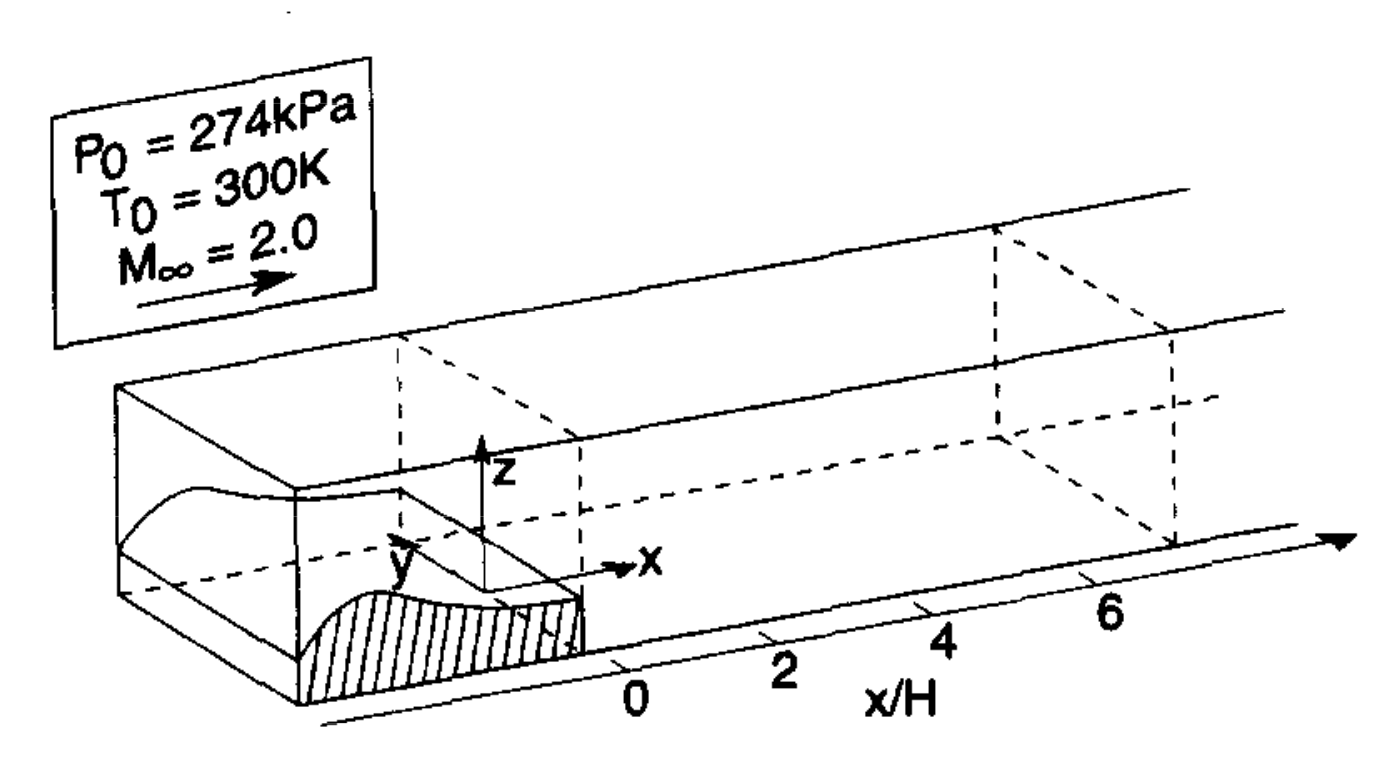
\includegraphics[width=12cm]{./chap4-backward-facing-step/figs/experimental-setup.png}
\end{center}
\caption{Schematic diagram of the experimental setup for the backward
         facing step test case (Reprinted from Eklund et. al. \cite{Eklund1995})}
\label{backward-facing-step-exp-setup-fig}
\end{figure}
%
A two-dimensional Laval nozzle designed to produce a Mach 2 exit flow was 
connected to the backward-facing step via a straight wall. This wall was
slightly angled at 0.5$^{\circ}$ to accommodate boundary layer growth. 
Table~\ref{backward-facing-step-test-section-dims} shows the 
dimensions of the test section in terms of the step height, $H$. The 
nominal inflow conditions of the test section are given in
Table~\ref{backward-facing-step-inflow-conditions}. The inflow boundary 
layer had a thickness of approximately 1.6 mm, and was verified to be 
fully developed and turbulent at one step height distance upstream of 
the step \cite{McDaniel1991}. 
%
\begin{table}[h]
  \caption{Test section geometry}
  \label{backward-facing-step-test-section-dims}
  \begin{center}
    \begin{tabular}{cc}
      \hline\hline
      Feature & Dimension \\
      \hline
      Step height         & $H$=3.175 mm \\
      Test section height & 6.71$H$  \\
      Test section width  & 9.6$H$   \\
      Step location       & $x/H$=0.0 \\
      \hline \hline
    \end{tabular}
  \end{center}
\end{table}
%
\begin{table}[h]
  \caption{Test section nominal inflow conditions}
  \label{backward-facing-step-inflow-conditions}
  \begin{center}
    \begin{tabular}{ccc}
      \hline\hline
      Parameter & & Freestream conditions \\
      \hline
      Stagnation pressure    & $P_0$      & 274 kPa \\     
      Stagnation temperature & $T_0$      & 300 K   \\   
      Mach number            & $T_0$      & 2.0     \\
      Static pressure        & $P_\infty$ & 35 kPa  \\  
      Static temperature     & $T_\infty$ & 167 K   \\
      $u$-velocity           & $u_\infty$ & 518 m/s \\
      \hline \hline
    \end{tabular}
  \end{center}
\end{table}
Three types of measurement techniques were used for flowfield measurements
in these experiments - pointwise Laser-Induced Iodine Fluorescence (LIIF),
Planar Laser-Induced Iodine Fluorescence (PLIIF) \cite{McDaniel1991, McDaniel1993} 
, and Laser Doppler Anemometry (LDA). LIIF 
techniques are non-intrusive optical techniques that infer flowfield
properties from signals resulting from the laser-induced fluorescence of
iodine molecules seeded into the flow. The pointwise LIIF technique was 
used to produce pointwise measurements of pressure, temperature and velocity
in the test section. In contrast to the pointwise LIIF technique, the PLIIF 
technique was used to produce planar measurements of pressure, temperature and 
velocity. Laser Doppler Anemometry, a well-established technique for pointwise
velocity measurement, was used in these experiments to measure the mean velocities 
and their fluctuations. Since the LIIF and PLIIF techniques provided only 
time-averaged data, the LDA data was an important addition to the data set in 
providing information about the turbulence intensity in the flow field.

Eilmer3 results are compared to profiles of pressure, temperature, and 
$u$-velocity obtained via the pointwise LIIF technique at seven positions along the 
centerline of the test section that correspond to $x/H$ locations of -1.0, -0.1, 1.7, 
3.0, 3.9, 6.7 and 10.8. The comparisons at $x/H$ = -1.0 are made to confirm that
Eilmer3 simulations of the inflow to the step are correct. Contour plots of pressure 
and temperature obtained numerically are also compared with planar measurements 
obtained via the PLIIF technique. 

The uncertainties of the various experimental techniques used in the 
acquisition of the data sets are listed in Table~\ref{backward-facing-step-uncertainties}. 
The uncertainties are quoted as a percentage of the freestream conditions in 
Table~\ref{backward-facing-step-inflow-conditions}. The actual 
uncertainties in the PLIIF images may be larger than those listed in 
Table~\ref{backward-facing-step-uncertainties} in certain regions of the image, as will be
discussed in Section~\ref{backward-facing-step-results}. Absolute spatial positioning error 
for all measurement techniques was less than $\pm$50 $\mu$m, or $\pm$1.6\% of the step 
height, $H$. 

%The spatial positioning was inherently more precise in the PLIIF 
%techniques than in the pointwise techniques. The spatial measurement volume 
%was approximately 0.001 mm$^3$ for the LIIF and PLIIF techniques and 
%approximately 0.01 mm$^3$ for the LDA technique. \\

\begin{table}
  \caption{Experimental uncertainties (from \cite{McDaniel1991}) }
  \label{backward-facing-step-uncertainties}
  \begin{center}
    \begin{tabular}{ccc}
      \hline\hline
      Technique & Parameter & Uncertainty \\
      \hline
      LIIF  & $P$ & $\pm$4\%\\
            & $T$ & $\pm$2\%\\
            & $u$ & $\pm$5\%\\
      PLIIF & $P$ & $\pm$6\%\\
            & $T$ & $\pm$5\%\\
            & $u$ & $\pm$2\%\\
      LDA   & $u$, $w$   & $\pm$2\%\\
            & $u'$, $w'$ & $\pm$2\%\\
      \hline \hline
    \end{tabular}
  \end{center}
\end{table}

%-----------------------------------------------------------------
\subsection{Details of computational approach}
%\label{}
%
The computational mesh used is shown in Figure~\ref{backward-facing-step-computational-mesh}.
Note that the Laval nozzle present in the experiments was not modelled. In place of this,
a two-dimensional duct with a 0.5$^{\circ}$ slope to accommodate boundary layer growth
was used. The overall length of the duct was adjusted until the simulated boundary
layer profiles match the experimentally measured profiles at $x/H$ = -1.0. The
turbulence intensity and turbulent-to-laminar viscosity ratio were also adjusted
so that the turbulence intensity matched that measured at $x/H$ = -1.0 using
the LDA technique. The turbulence intensity and turbulent-to-laminar viscosity ratio used
for these simulations are 1\% and 100 respectively. Since the turbulence intensity and 
turbulent-to-laminar viscosity ratio were also fixed, sensitivity studies of the results 
to these freestream turbulence properties were not conducted.

The inflow parameters were specified as per Table~\ref{backward-facing-step-inflow-conditions}. 
Air with an ideal gas assumption, a constant specific heats ratio of 1.4 and a 
gas constant of 287.1 J/kg.K was used as the test gas for the simulations.
\begin{figure}[h]
 \begin{center}
  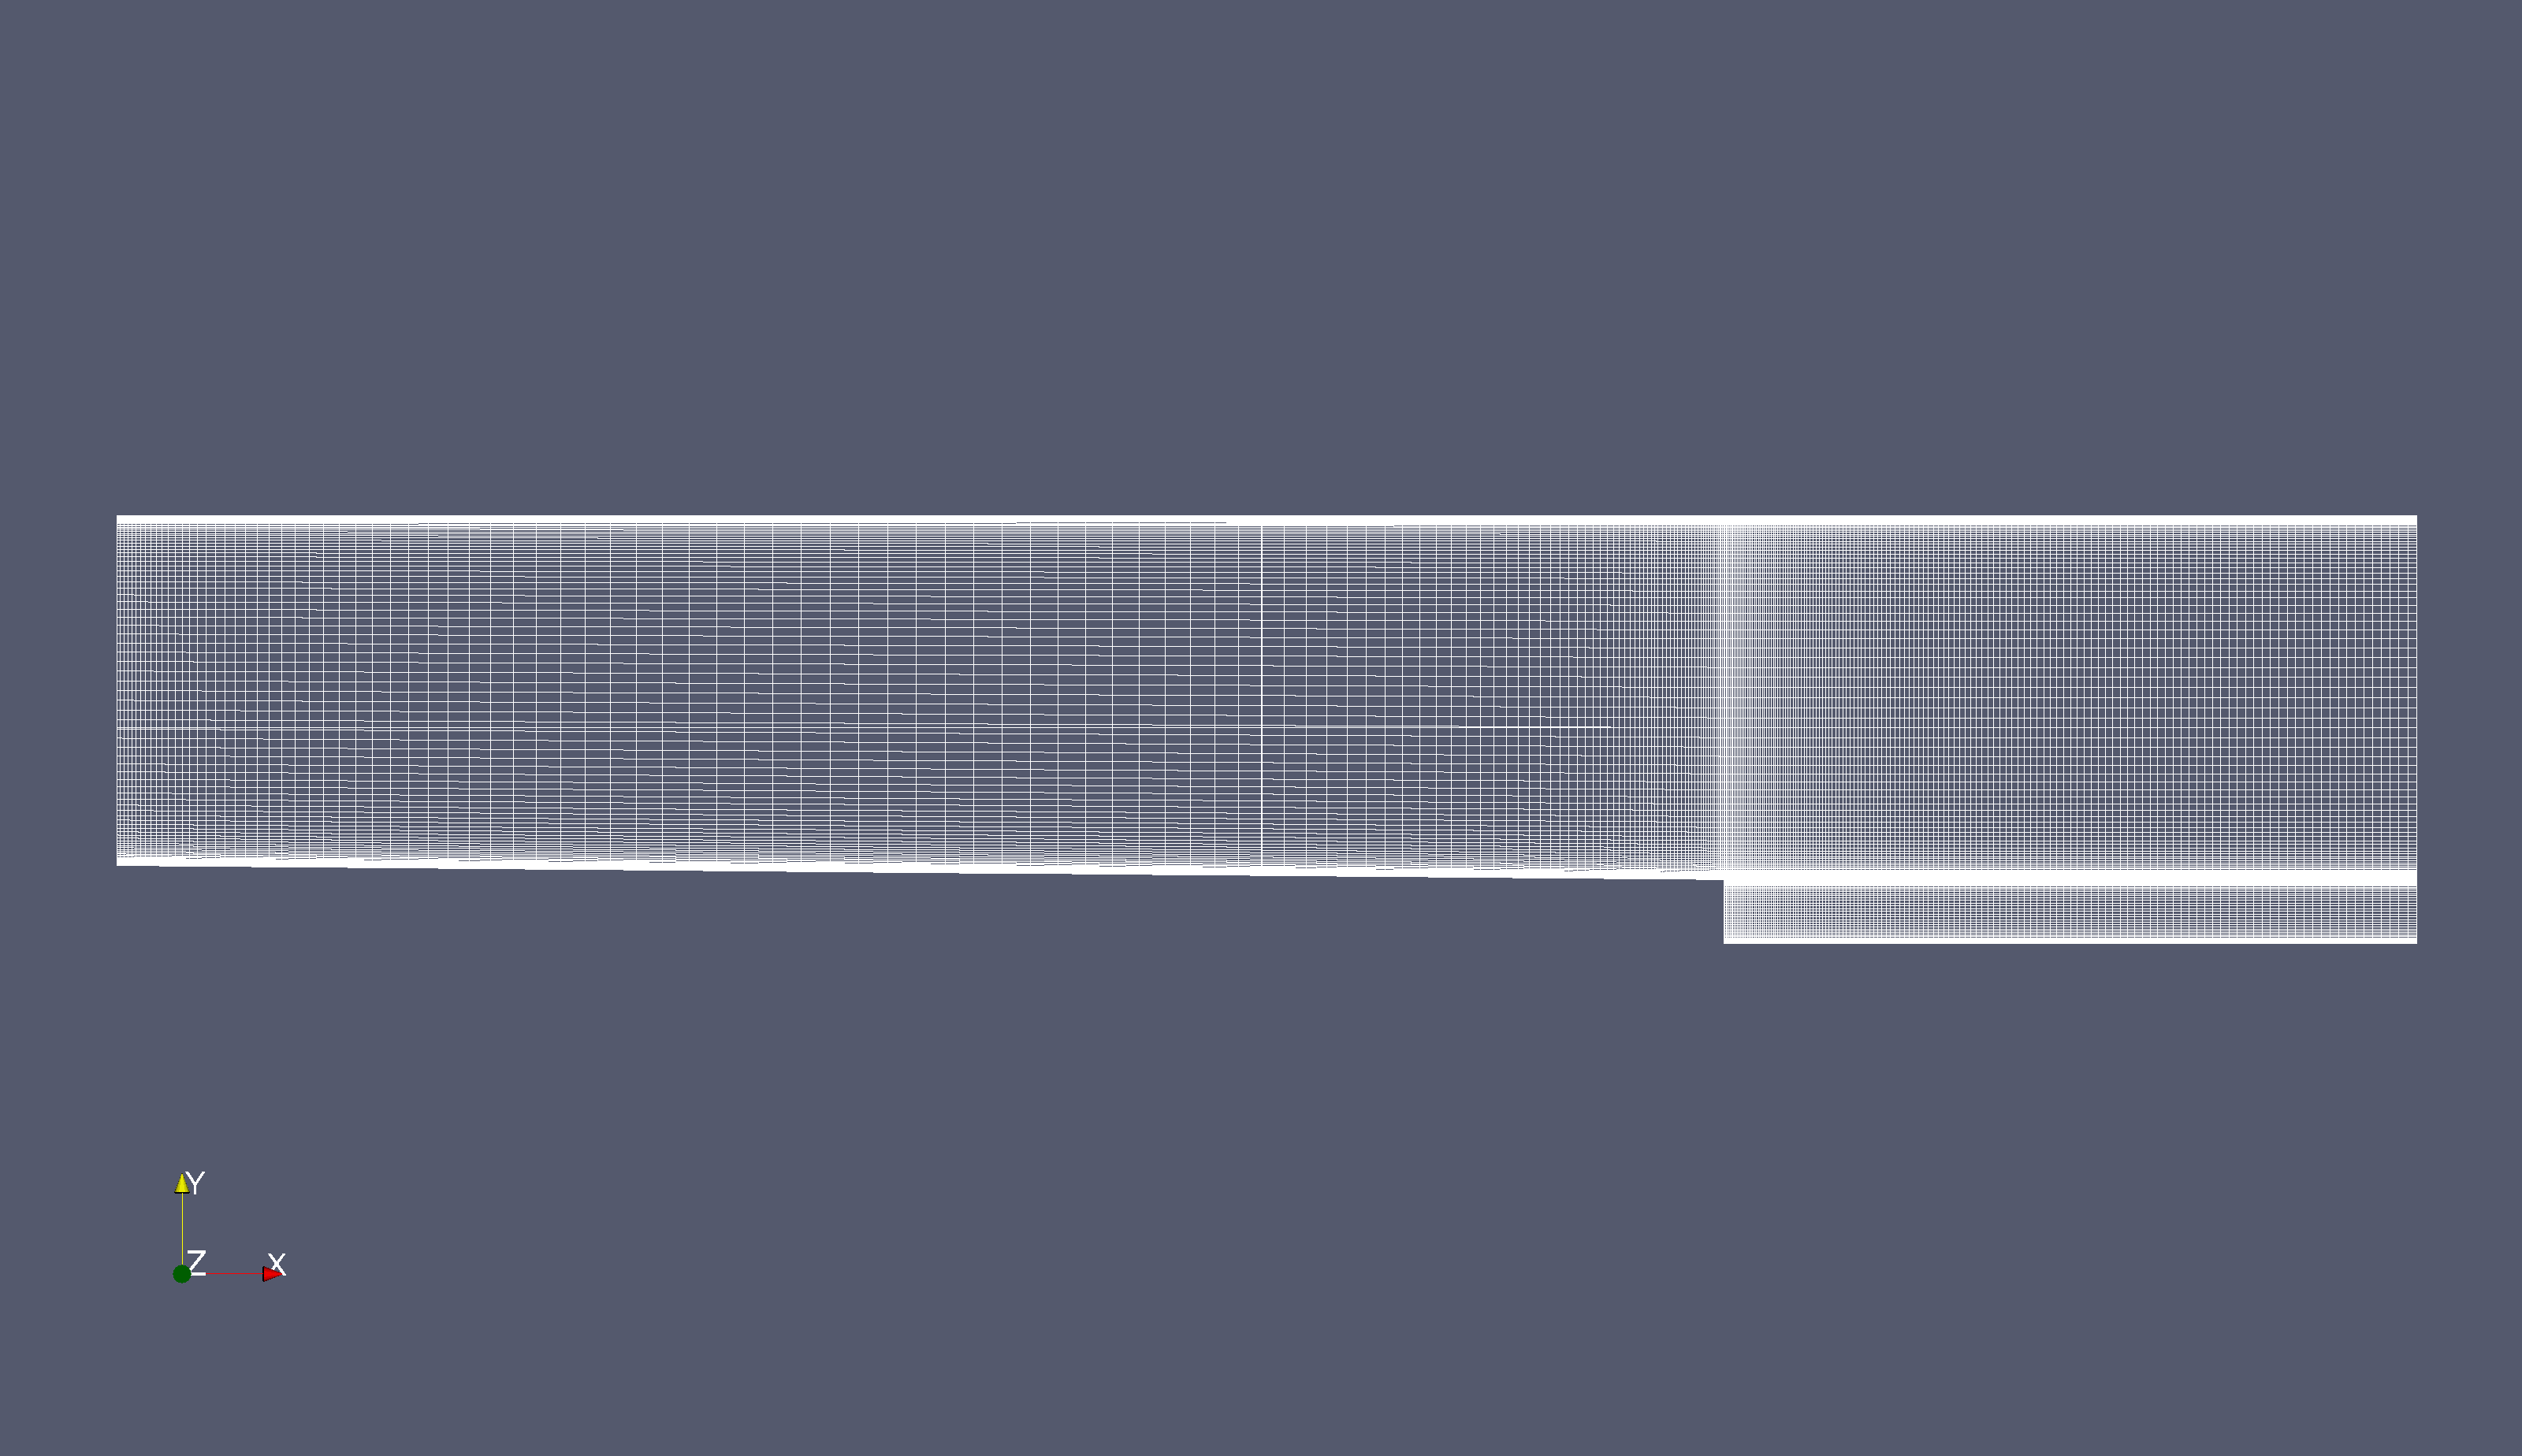
\includegraphics[width=10cm]{./chap4-backward-facing-step/figs/grid.png}
 \end{center}
 \caption{Computational mesh}
 \label{backward-facing-step-computational-mesh}
\end{figure}
Three sets of grids were used for this test case - a fine grid (40080 cells), 
a medium grid (10020 cells), and a coarse grid (2685 cells). The $y^+$ (or $z^+$ 
for the coordinate system used in this section) for the grids were lesser than 1.0, 
except in the first few wall cells from the leading edge where the boundary layer 
was establishing. It was also ensured that there were at least 15 cells within the
boundary layer for most parts of the computational domain.

%-----------------------------------------------------------------
\subsection{Grid convergence}
%\label{}
%
Figures~\ref{backward-facing-step-xH--01} - \ref{backward-facing-step-xH-108}
show that sufficiently grid-resolved results can be obtained from Eilmer3 simulations
using the fine grid.

%------------------------------------------------------------------
\subsection{Results \& discussions}
\label{backward-facing-step-results}
%
Comparisons between numerical predictions and experimental data are firstly
made for the inflow upstream of the step at $x/H$ = -1.0. Comparisons will then
be made with the PLIIF measurements and with the pointwise LIIF measurements.

A comparison of the numerical and experimental profiles at one step height
($x/H$ = -1.0) upstream of the step is shown in Figure~\ref{backward-facing-step-xH--10}.
Three minor discrepancies can be observed. Firstly, the numerical simulations did not
predict as much fluctuations in the pressure level as in the experimental data.
Considering that the actual 2D Laval nozzle was not being modelled due to the 
unavailability of nozzle geometrical information, and that the average pressure
levels matches the experimental data, this discrepancy is deemed acceptable. Secondly,
the numerical simulations seem to overpredict the temperature in the region
near the walls. For the PLIIF technique employed, the fluorescence signal 
decreases with increasing temperature. For this reason, an increment in the measured 
signal owing to background scattering near tunnel walls can substantially lower measured
temperatures \cite{Eklund1995}. These low temperature measurements in the region near the wall
can be consistently seen in later comparisons made with PLIIF and LIIF data. Thirdly,
despite matching the turbulence intensity levels in the freestream of the flow,
the turbulence intensity near the walls are underpredicted. The experimental 
turbulence intensity is the root-mean-square value of $u$-velocity fluctuations
normalised by freestream $u$-velocity, $\sqrt{u^{'2}}/u_{\infty}$, while 
the numerical turbulence intensity is the square-root of two-thirds of the turbulence 
kinetic energy normalised by freestream $u$-velocity, $\sqrt{\frac{2}{3}k}/u_{\infty}$. 
The assumption that $\sqrt{u^{'2}}$ is equal to $\sqrt{\frac{2}{3}k}$ is only valid if
the turbulence is isotropic. However, in most turbulent shear flows, where turbulence
is anisotropic, $\sqrt{u^{'2}}$ is slightly larger than $\sqrt{\frac{2}{3}k}$ \cite{Hinze1975}.
As such. the comparison between experimental and numerical turbulence intensities
in Figure~\ref{backward-facing-step-xH--10} should only be treated as an
approximate one. Apart from these discrepancies, the overall agreement between the
numerical and experimental profiles upstream of the step is excellent. This allows
a more confident assessment of the numerical predictions of the flow past the step
to be made.
%
\begin{figure}[h]
 \begin{center}
  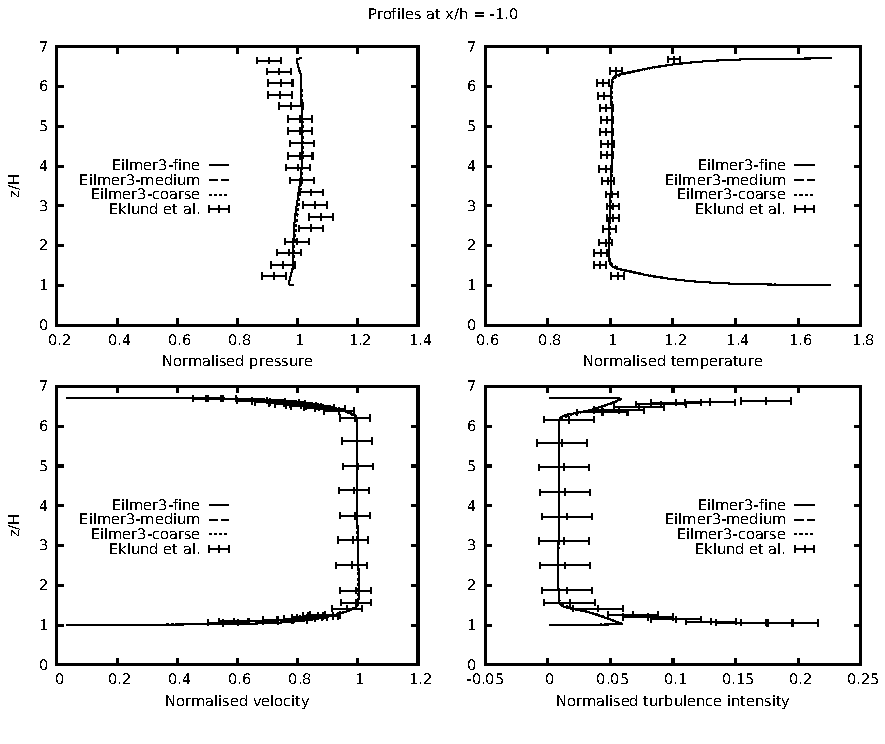
\includegraphics[width=15cm]{./chap4-backward-facing-step/figs/xh_-10.pdf}
 \end{center}
 \caption{Boundary layer profiles at $x/H$ = -1.0}
 \label{backward-facing-step-xH--10}
\end{figure}
%

Eilmer3 predictions of flow past the step are shown together with experimental
PLIIF measurements in Figures~\ref{figure-backward-step-pressure-contours} and 
\ref{figure-backward-step-temperature-contours}. 
Figure~\ref{figure-backward-step-pressure-contours} shows that the
%
\begin{figure}[h]
 \centering
 \subfigure[]{
   \label{figure-backward-step-pressure-contours-a}
   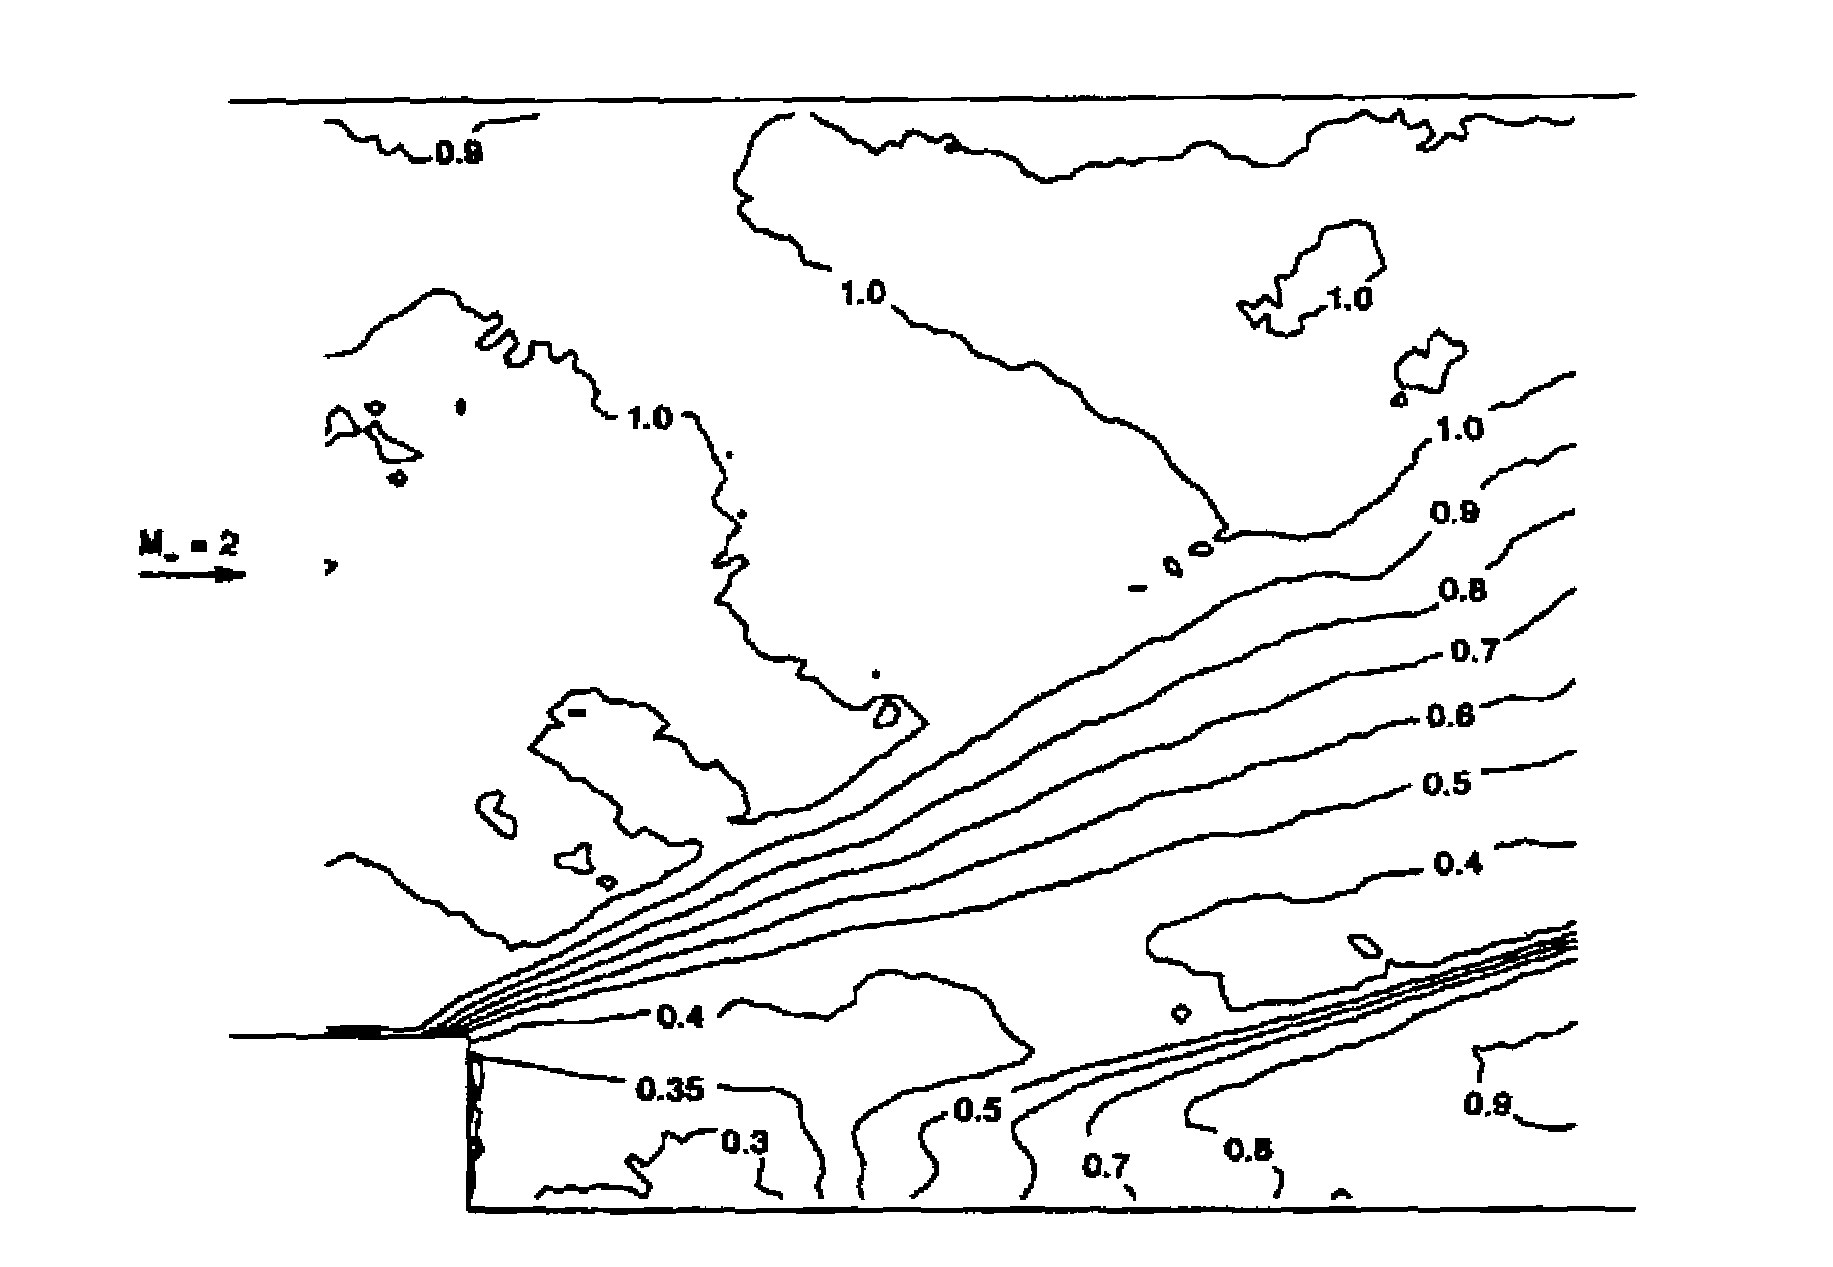
\includegraphics[width=14cm]{./chap4-backward-facing-step/figs/pressure_contours_exp.pdf}
 }
 \subfigure[]{
   \label{figure-backward-step-pressure-contours-b}
   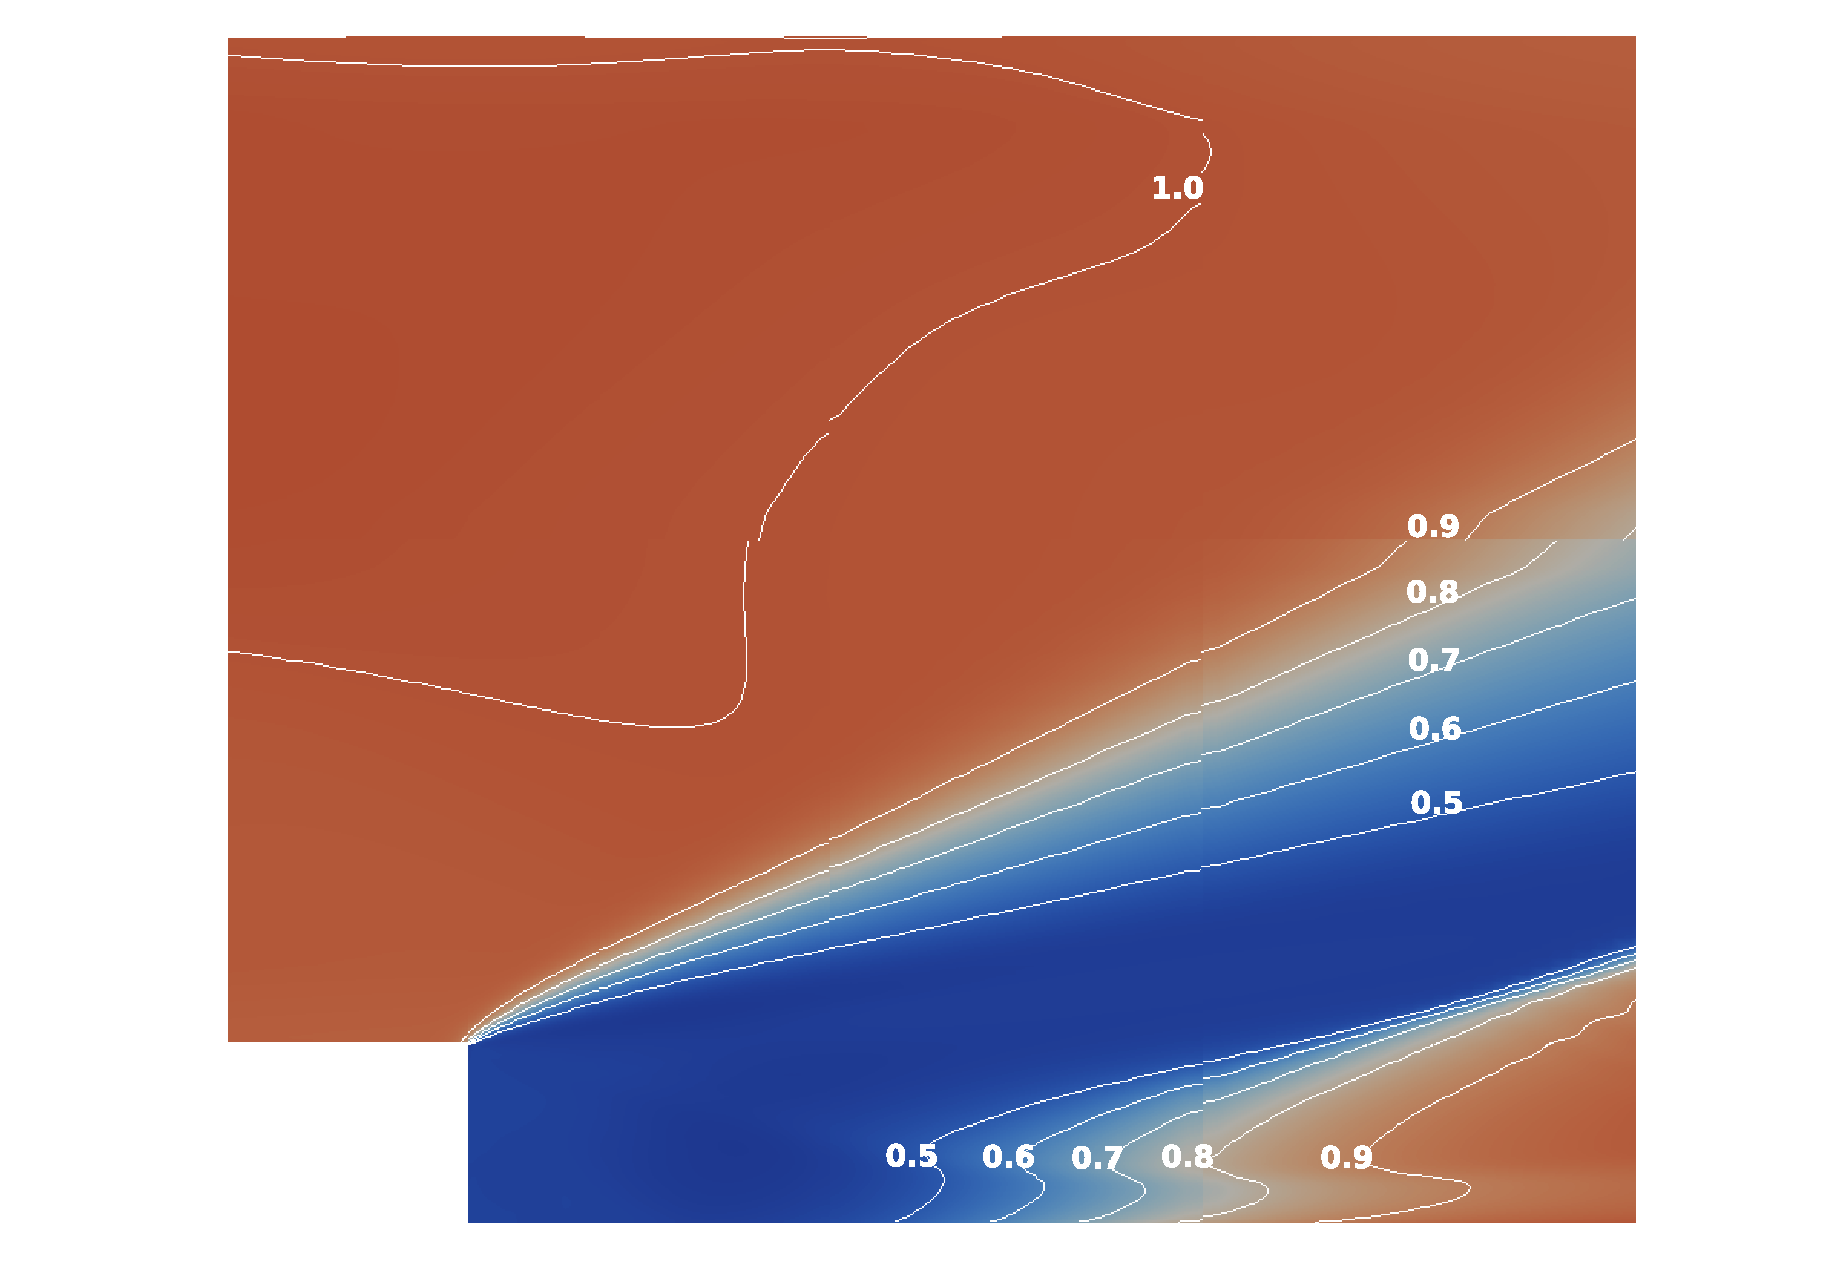
\includegraphics[width=14cm]{./chap4-backward-facing-step/figs/pressure_contours_num.pdf}
 }
 \caption{Comparison between (a) experimentally measured and (b)
          numerically simulated pressure contours}
 \label{figure-backward-step-pressure-contours}
\end{figure}
%
\begin{figure}[h]
 \centering
 \subfigure[]{
   \label{figure-backward-step-temperature-contours-a}
   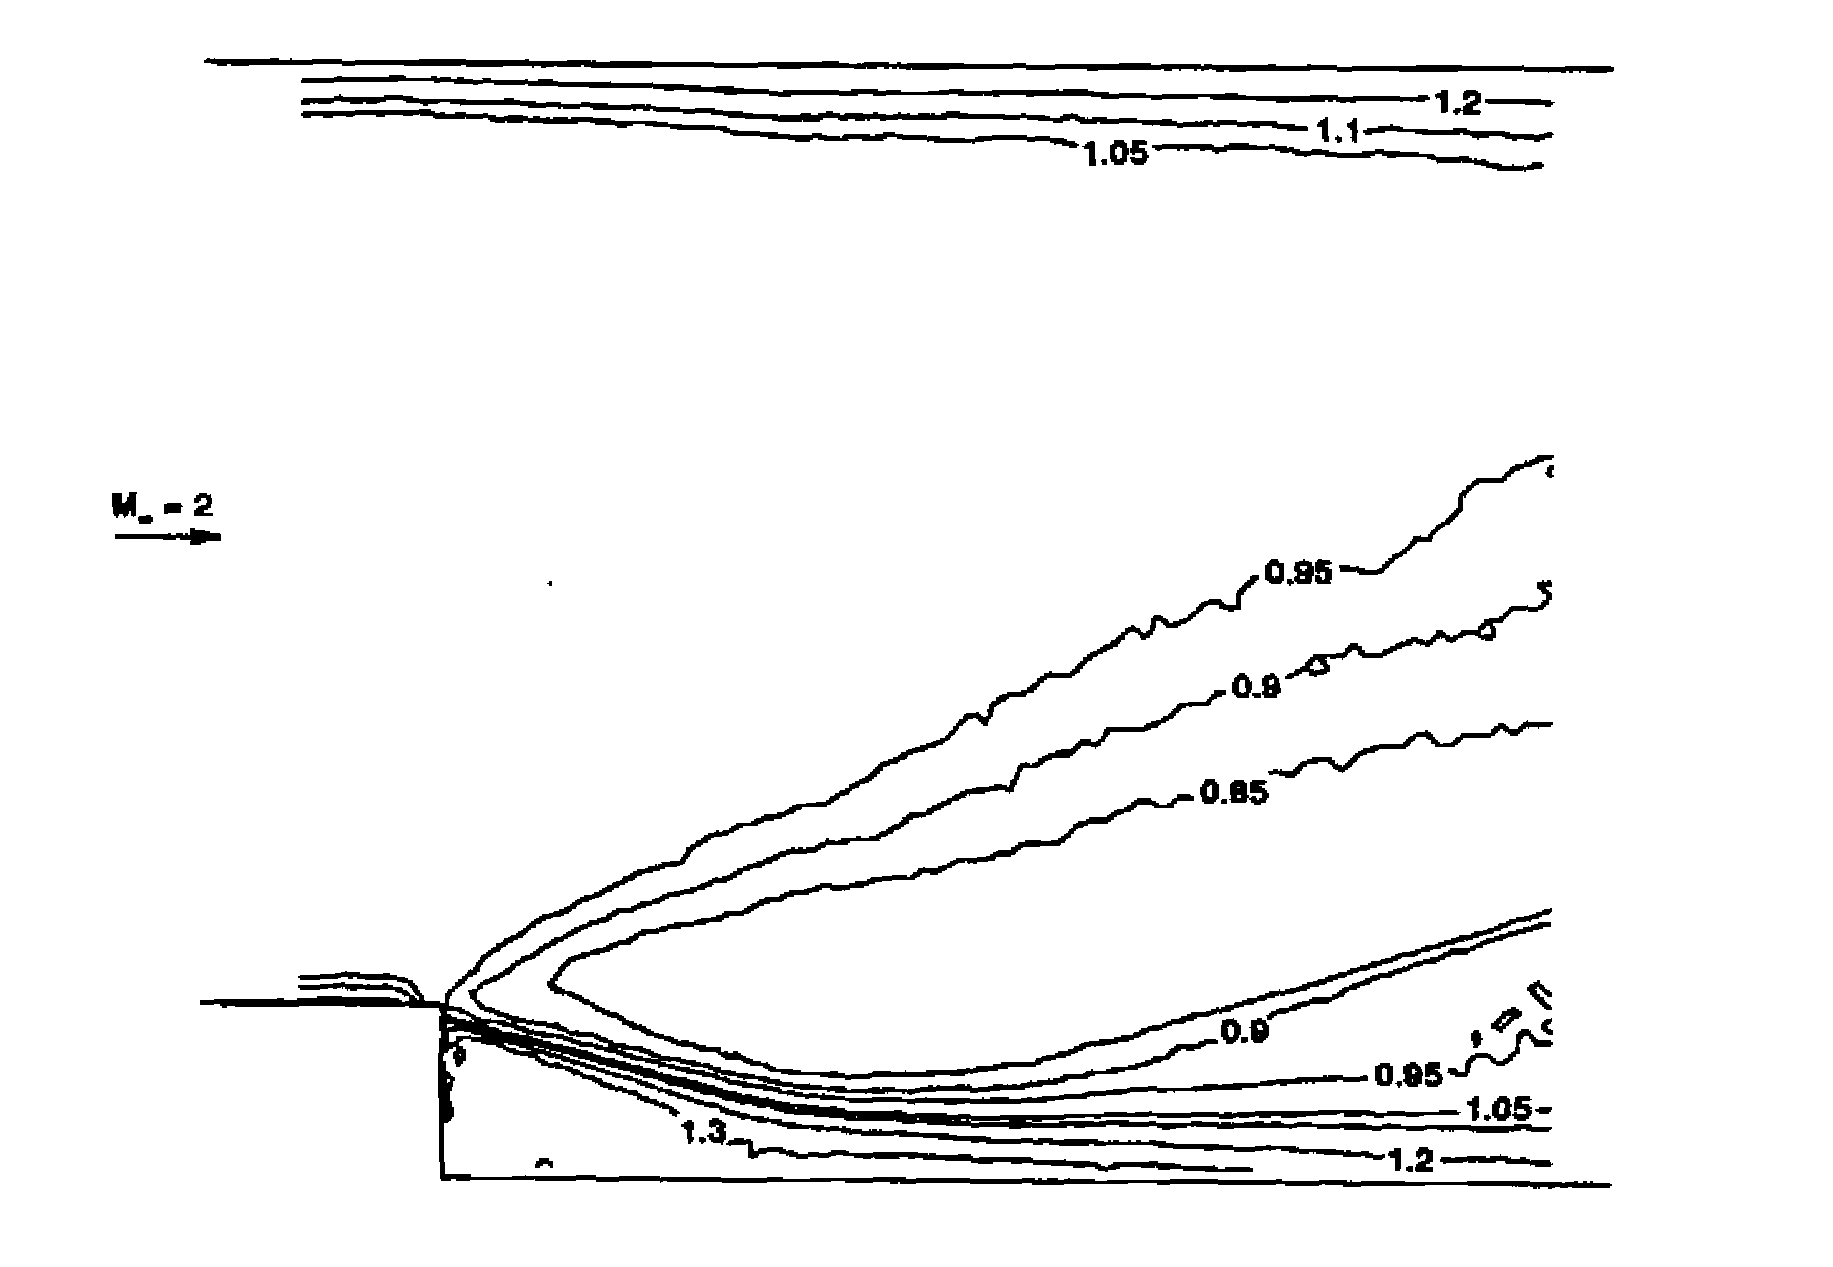
\includegraphics[width=14cm]{./chap4-backward-facing-step/figs/temperature_contours_exp.pdf}
 }
 \subfigure[]{
   \label{figure-backward-step-temperature-contours-b}
   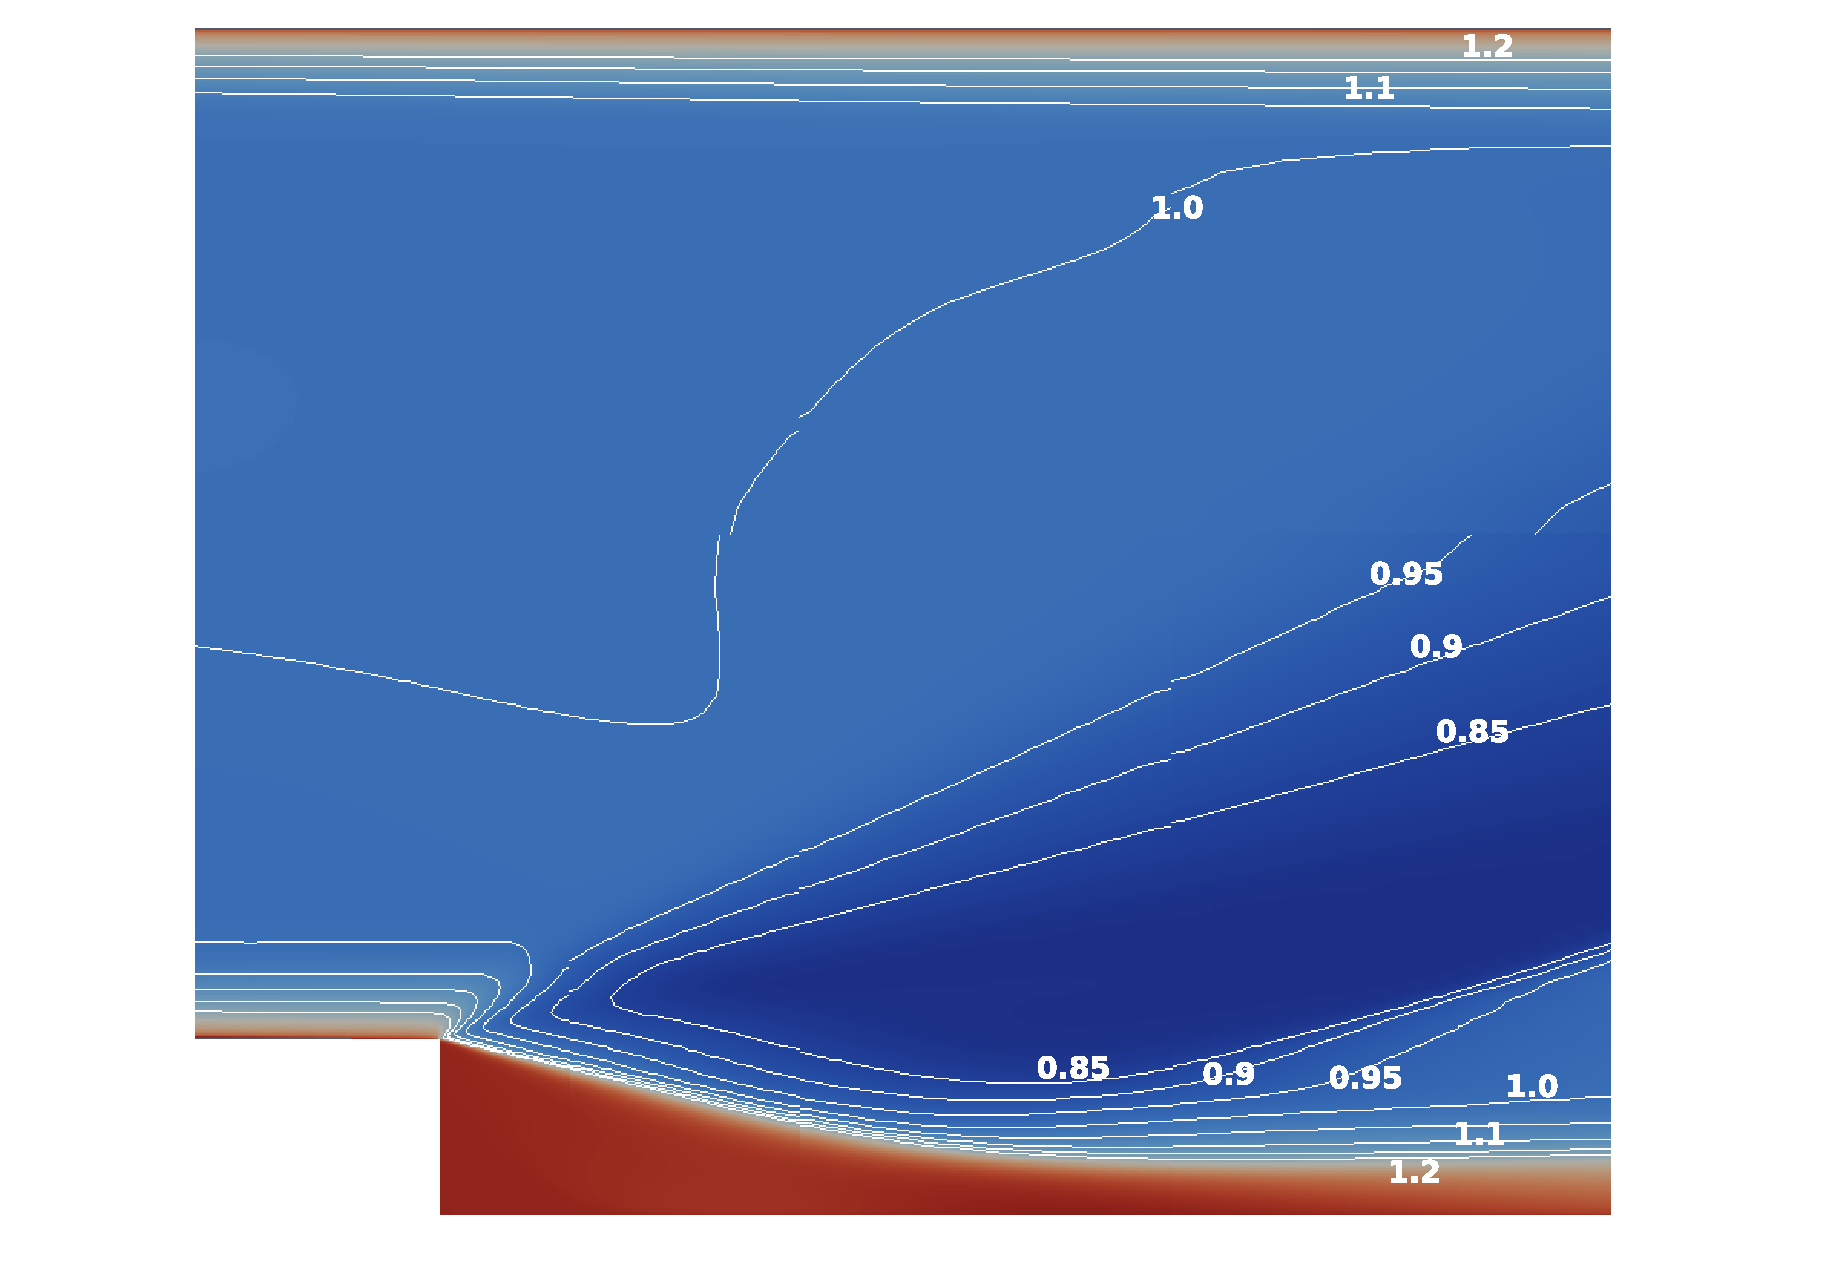
\includegraphics[width=14cm]{./chap4-backward-facing-step/figs/temperature_contours_num.pdf}
 }
 \caption{Comparison between (a) experimentally measured and (b)
          numerically simulated temperature contours}
 \label{figure-backward-step-temperature-contours}
\end{figure}
%
degree of expansion and reattachment shock angle are well predicted. Only 
two minor differences can be seen. Firstly, the expansion fan is predicted 
to centre around the step and does not extend as far upstream as measured 
in the experiments. Eklund et. al. \cite{Eklund1995} explained
that the occurence of the expansion fan further upstream of the step was
attributed to the suction effect from the low pressure region in the base region
of the step. This phenomena is not predicted by the Eilmer3 simulations probably because
the slight curvature that was present at the corner of the step was not modelled. 
This curvature was mentioned in the paper of Eklund et. al. \cite{Eklund1995}, but no geometrical
information was provided. The second difference is that the recompression is predicted 
to begin further upstream than in the experimental PLIIF measurements. This is 
despite the recompression shock angle being predicted correctly. This results in 
higher pressure levels in the vicinity.
Figure~\ref{figure-backward-step-temperature-contours} shows good agreement between 
the predicted and measured temperatures everywhere in the flowfield other than in 
the region near the walls. As discussed earlier, Eilmer3 predicts higher temperature 
levels than measured. This mismatch is due to the erroneous near-wall PLIIF measurement 
of temperatures brought about by background scattering.

Comparisons between the predicted and measured profiles of pressure, temperature
and $u$-velocity at several axial locations are shown in Figures~\ref{backward-facing-step-xH--01} - \ref{backward-facing-step-xH-108}.
The good agreement observed earlier between Eilmer3 predictions and PLIIF measurements
is also seen when comparing the predictions with pointwise LIIF measurements.
The differences observed earlier can also be seen in this comparison. 
The discrepancy in the prediction of the origin of the expansion fan can be seen in
the pressure profiles at $x/H$ = -0.1. The start of recompression shock is however 
different from the PLIIF comparisons, with it being predicted to occur downstream, 
as shown at $x/H$ = 3.9. The systematically low temperatures measured in the vicinity 
of the wall is seen again at every axial location. In summary, the overall agreement of 
Eilmer3 predictions with the experimental data is excellent.
%
\begin{figure}[h]
 \begin{center}
  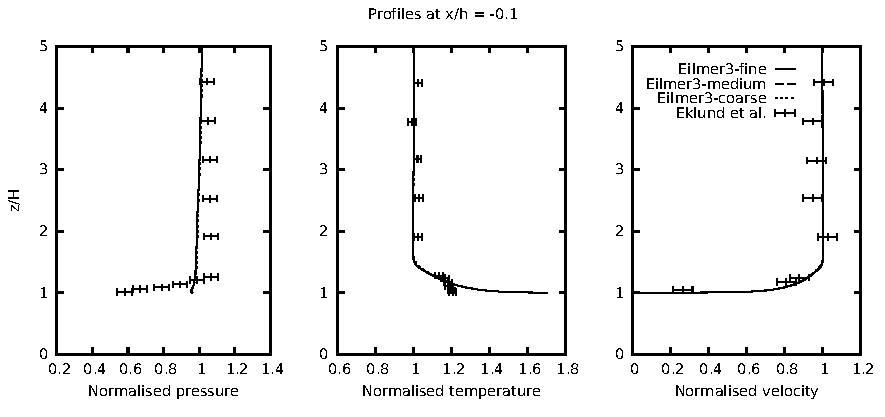
\includegraphics[width=13.8cm]{./chap4-backward-facing-step/figs/xh_-01.pdf}
 \end{center}
 \caption{Boundary layer profiles at $x/H$ = -0.1}
 \label{backward-facing-step-xH--01}
\end{figure}
%
\begin{figure}[h]
 \begin{center}
  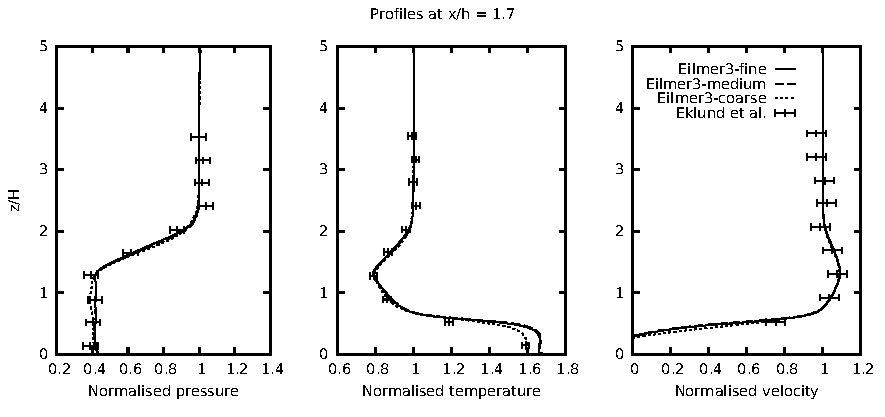
\includegraphics[width=13.8cm]{./chap4-backward-facing-step/figs/xh_17.pdf}
 \end{center}
 \caption{Boundary layer profiles at $x/H$ = 1.7}
 \label{backward-facing-step-xH-17}
\end{figure}
%
\begin{figure}[h]
 \begin{center}
  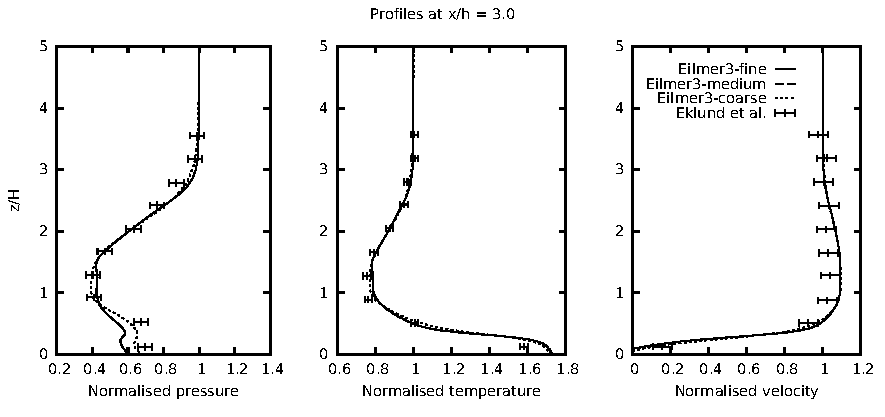
\includegraphics[width=13.8cm]{./chap4-backward-facing-step/figs/xh_30.pdf}
 \end{center}
 \caption{Boundary layer profiles at $x/H$ = 3.0}
 \label{backward-facing-step-xH-30}
\end{figure}
%
\begin{figure}[h]
 \begin{center}
  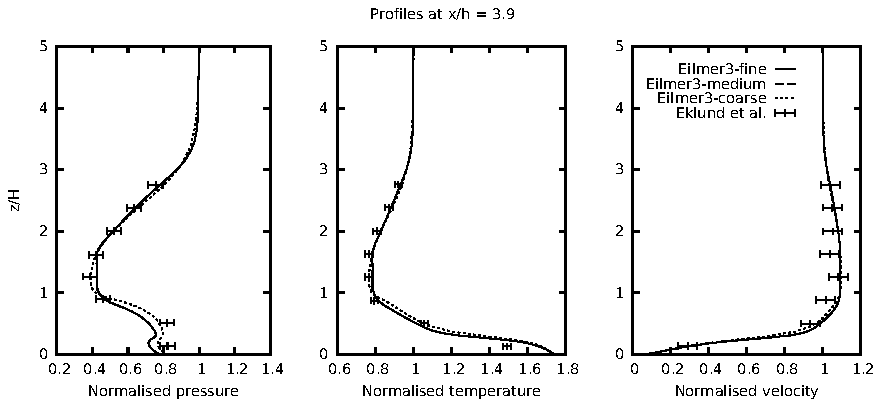
\includegraphics[width=13.8cm]{./chap4-backward-facing-step/figs/xh_39.pdf}
 \end{center}
 \caption{Boundary layer profiles at $x/H$ = 3.9}
 \label{backward-facing-step-xH-39}
\end{figure}
%
\begin{figure}[h]
 \begin{center}
  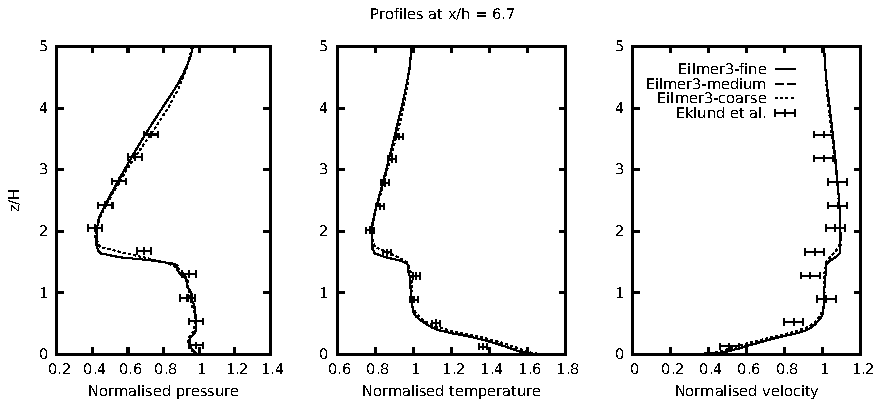
\includegraphics[width=13.8cm]{./chap4-backward-facing-step/figs/xh_67.pdf}
 \end{center}
 \caption{Boundary layer profiles at $x/H$ = 6.7}
 \label{backward-facing-step-xH-67}
\end{figure}
%
\begin{figure}[h]
 \begin{center}
  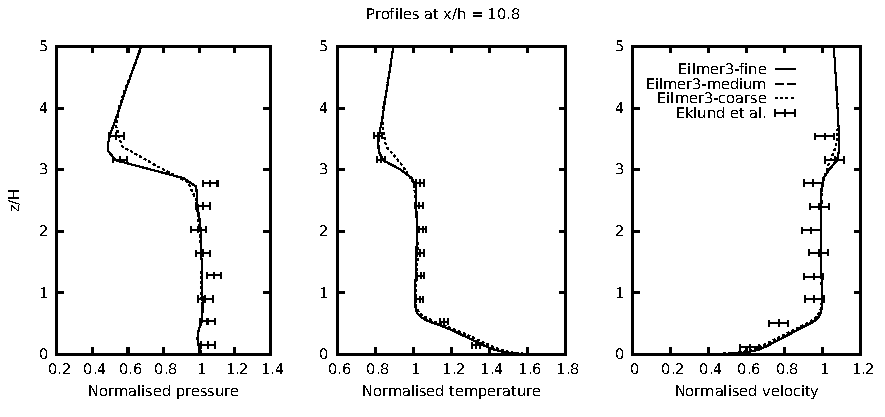
\includegraphics[width=13.8cm]{./chap4-backward-facing-step/figs/xh_108.pdf}
 \end{center}
 \caption{Boundary layer profiles at $x/H$ = 10.8}
 \label{backward-facing-step-xH-108}
\end{figure}
%

%------------------------------------------------------------------



% coaxial-jets.tex

\newpage
\section{Turbulent mixing of supersonic coaxial jets}
\label{chapter-coaxial-jets}
%
This chapter reports the validation of experiments involving the 
turbulent mixing of supersonic coaxial jets. Conducted at NASA 
Langley Research Centre, these experiments have been adopted by
the NATO Research and Technology Organisation Working Group 10 
(Subgroup 2) as a test case for their CFD development and validation
activity. More details about this test case can be found in Cutler et. al. \cite{Cutler2006}.

%------------------------------------------------------------------
\subsection{Details of flow problem}
%\label{}
%
The experimental setup used by Cutler et al. is shown 
schematically in Figure~\ref{figure-coaxial-jets-exp-setup}.
The assembly, designed to discharge two coaxial jets into 
stagnant air, was axisymmetric and consisted of an outer
body and centre body. The passage between both bodies formed
an exit nozzle for the coflow jet while the the interior passage
of the centre body formed an exit nozzle for the centre jet. Both 
%
\begin{figure}[htbp]
\begin{center}
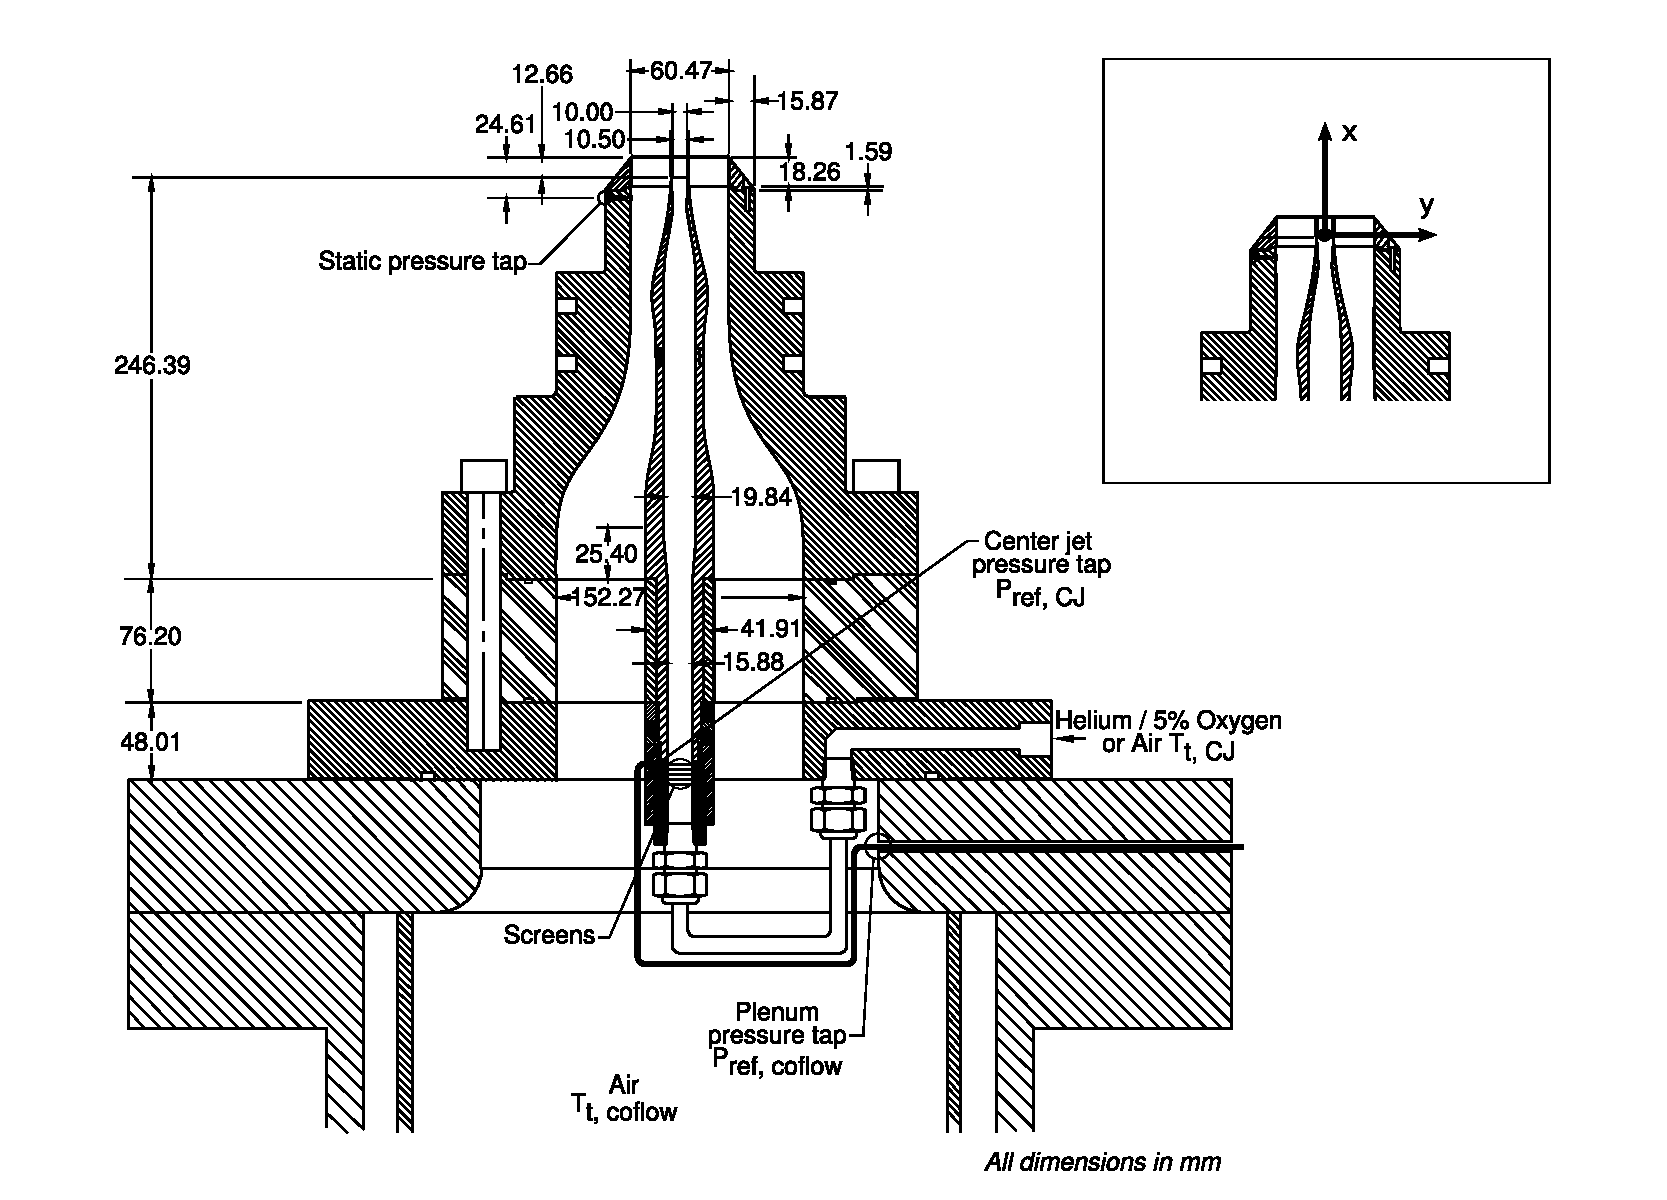
\includegraphics[width=15cm]{./chap5-coaxial-jets/figs/facility1-test.pdf}
\end{center}
\caption{Schematic diagram of experimental setup for coaxial jets test 
         case (Reprinted from \cite{Cutler2006}). Inset diagram 
         shows the coordinate system used in the Eilmer3 simulations.}
\label{figure-coaxial-jets-exp-setup}
\end{figure}
%
nozzle passages were designed using Method-of-Characteristics calculations to 
produce one-dimensional flow at the exit plane. The centre jet
consisted of a mixture of helium and oxygen (95\% He and 5\% O$_2$ by
volume, 70.4\% He and 29.6\% O$_2$ by mass), while the coflow jet 
surrounding the centre jet consisted of air. The presence of oxygen 
in the centre jet was to allow the use of an oxygen flow tagging 
technique (RELIEF) to obtain non-intrusive velocity measurements 
in the flow. Values of ambient pressure and temperature, reservoir 
pressure and temperature, and nozzle exit pressure are shown in 
Table~\ref{given-conditions-coaxial-jet}. 
%
\begin{table}[h]
  \caption{Ambient, reservoir and nozzle exit conditions}
  \label{given-conditions-coaxial-jet}
  \begin{center}
    \begin{tabular}{cccl}
      \hline\hline
      Parameter & Value   & Units \\
      \hline
      $P_{amb}$             & 101.9   & kPa \\
      $T_{amb}$             & 294.6   & K   \\
      $P_{res, \,\, coflow}$     & 580.0   & kPa \\
      $T_{res, \,\, coflow}$     & 300.0   & K   \\
      $P_{res, \,\, centrejet}$  & 614.8   & kPa \\
      $T_{res, \,\, centrejet}$  & 306.0   & K   \\
      $P_{nozzle \,\, exit, \,\, coflow}$     & 101.3   & kPa \\
      $P_{nozzle \,\, exit, \,\, centrejet}$     & 101.3   & kPa \\
      \hline \hline
    \end{tabular}
  \end{center}
\end{table}
%
Note that the exit pressure for both the coflow and centre jet
nozzles are similar. This set of experiments is considered to be 
an excellent test for the turbulence model since the streamwise 
development of the flow is dominated by turbulent stresses rather 
than pressure forces \cite{Cutler2001}.

Cylindrical pitot probes were used to measure pitot pressure. 
The mole fraction of the He-O$_2$ mixture was measured by processing 
the gas withdrawn from the flow by gas sampling probes with a hot-film 
probe-based system. The mean axial velocity and rms fluctuations were 
measured using the Raman-Excitation-plus-Laser-Induced-Electronic-Fluorescence (RELIEF) 
O$_2$ flow-tagging technique. The uncertainties in pitot pressure, 
helium-oxygen mole fractions, flow velocity, and rms fluctuations are 
\textbf{$\pm$??5?\%}, $\pm$1.5\%, $\pm$3\% and $\pm$3\% respectively.
Experimentally measured pitot pressure, He-O$_2$ mole fractions,
flow velocity, and turbulence intensity are compared with those
obtained from Eilmer3 simulations.

\subsection{Details of computational approach}
%\label{}
%
The grid used is shown in Figure~\ref{figure-coaxial-jets-grid}. The 
grid clustering towards the walls of both nozzles had been adjusted 
such that $y^+<1$. Grid clustering was also concentrated near the 
exit planes of both nozzles. This was done to capture the nozzle
lip shocks and expansions.
%
\begin{figure}[h]
 \centering
 \subfigure[]{
   \label{figure-coaxial-jets-overall-grid}
%   \fbox{Contents of first subfigure}
   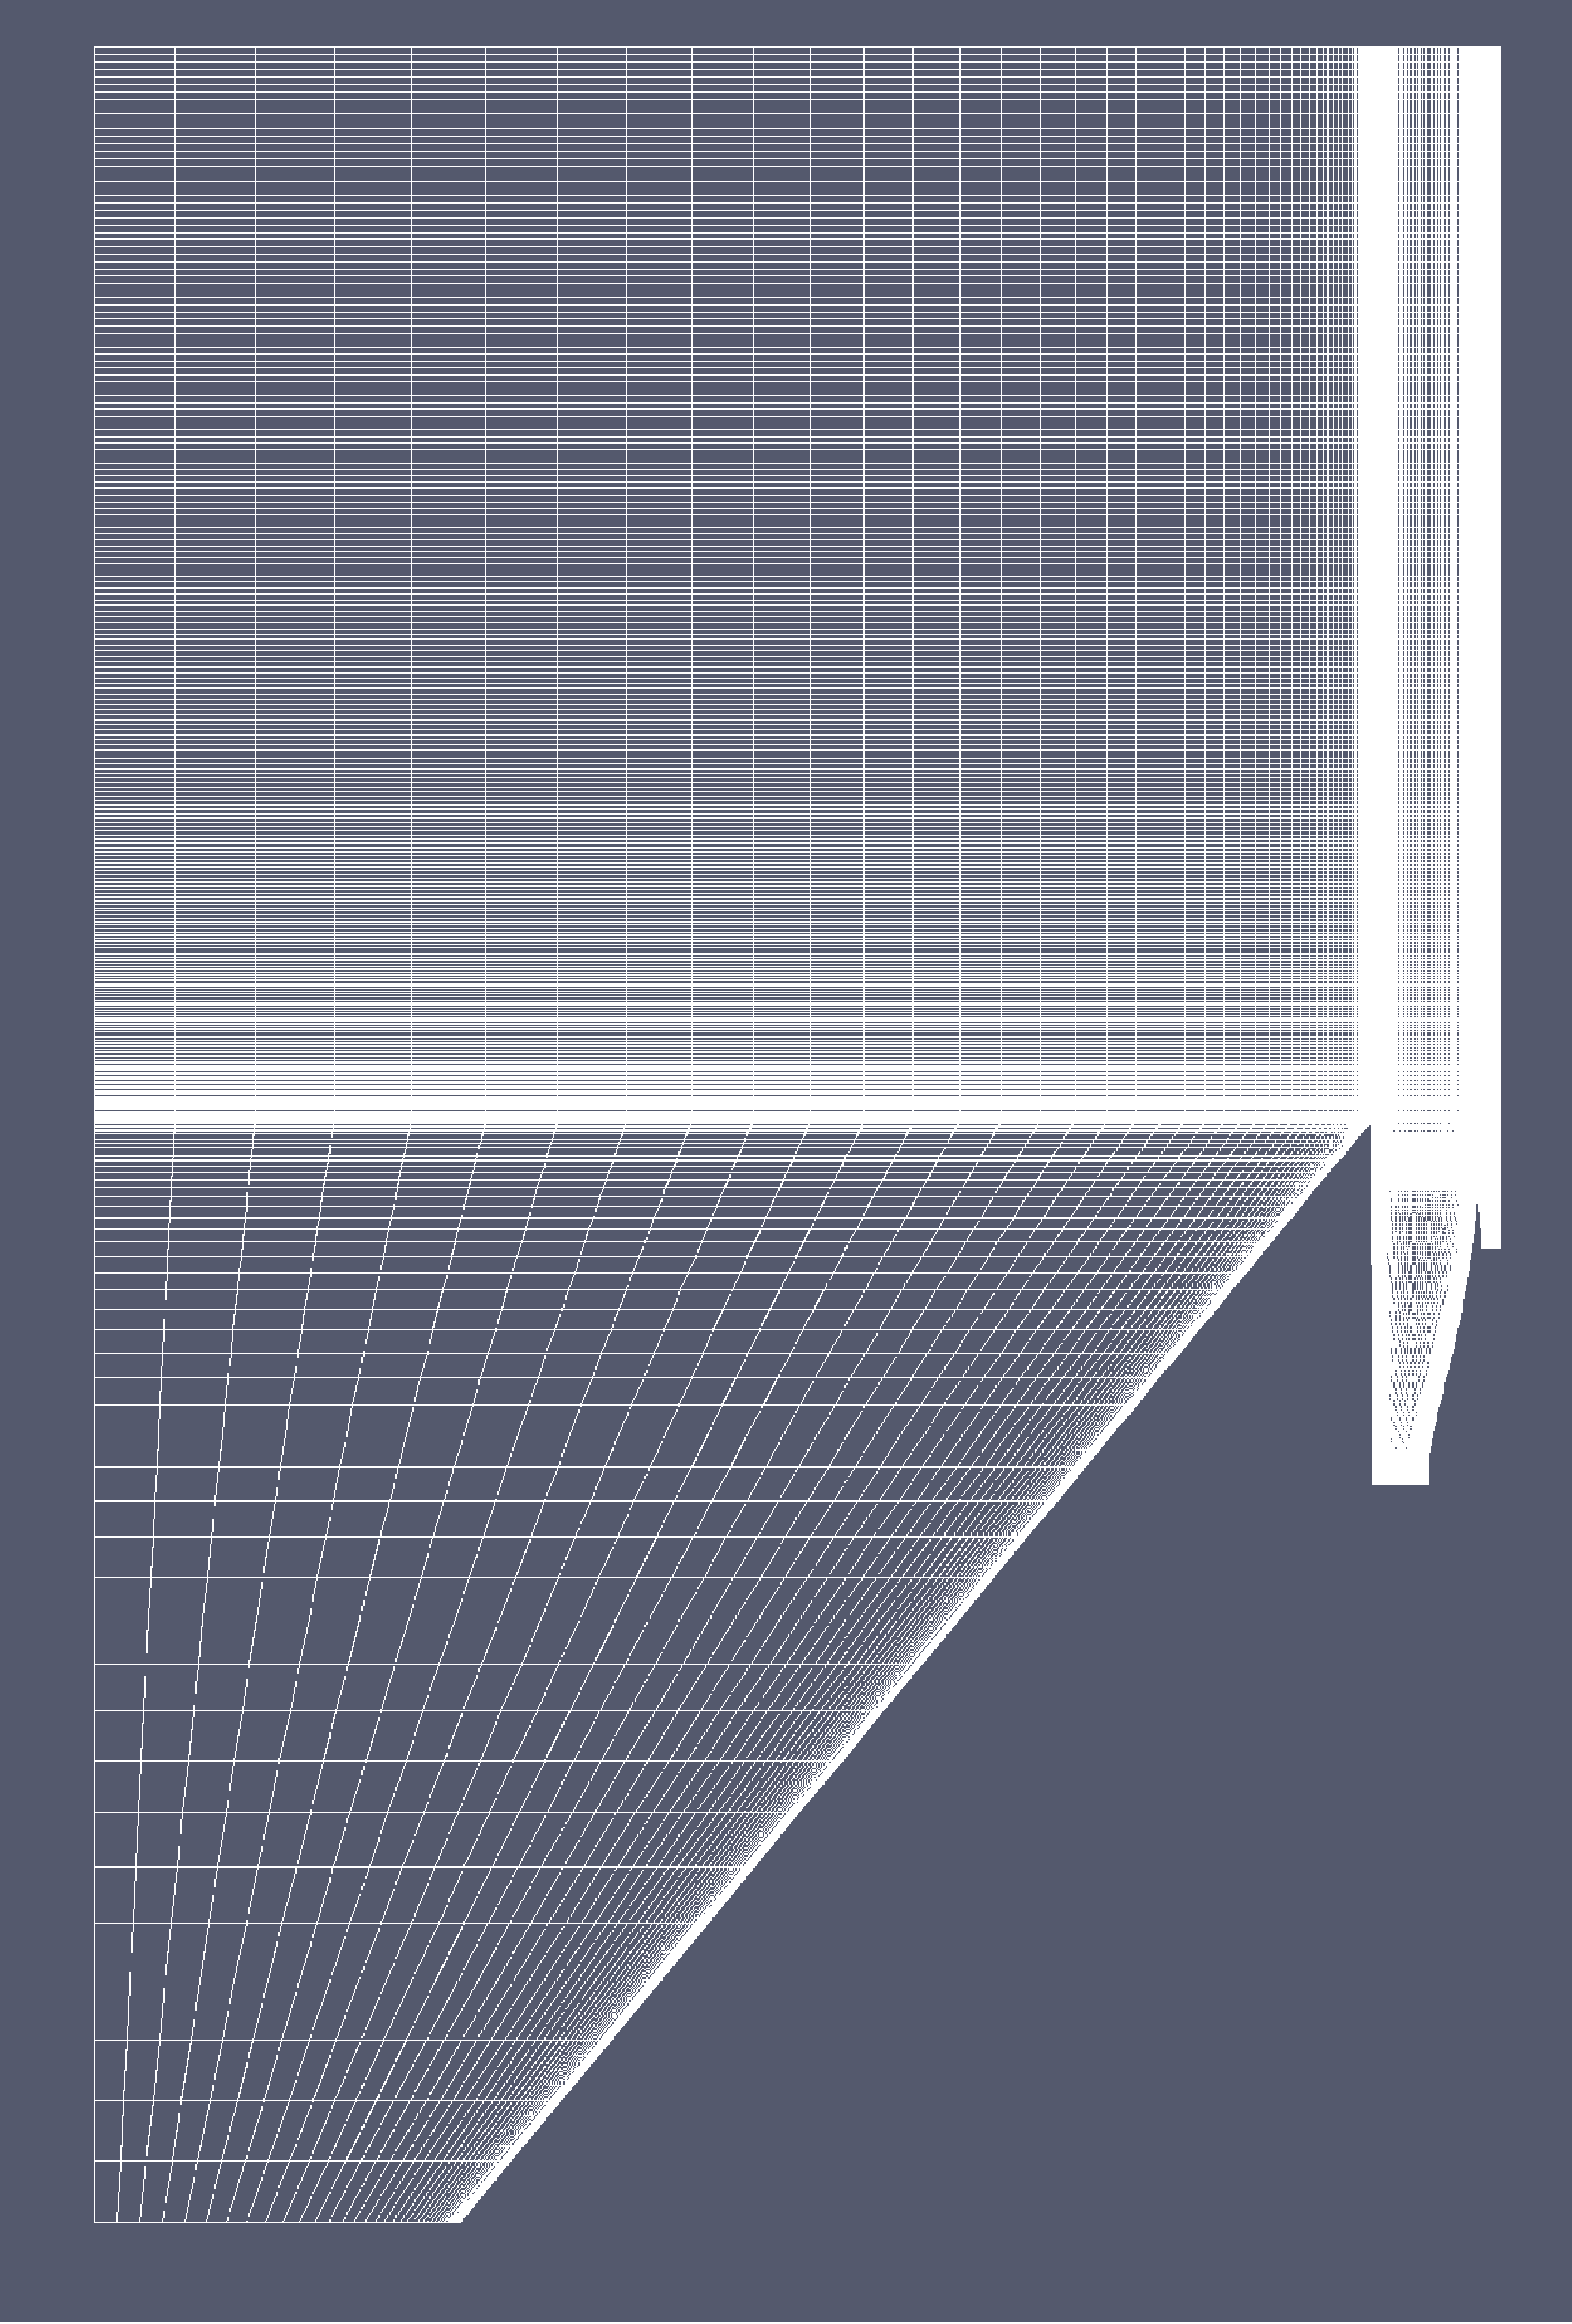
\includegraphics[width=7cm]{./chap5-coaxial-jets/figs/grid1.pdf}
 }
 \subfigure[]{
   \label{figure-coaxial-jets-zoomed-in-grid}
%   \fbox{Contents of second subfigure}
 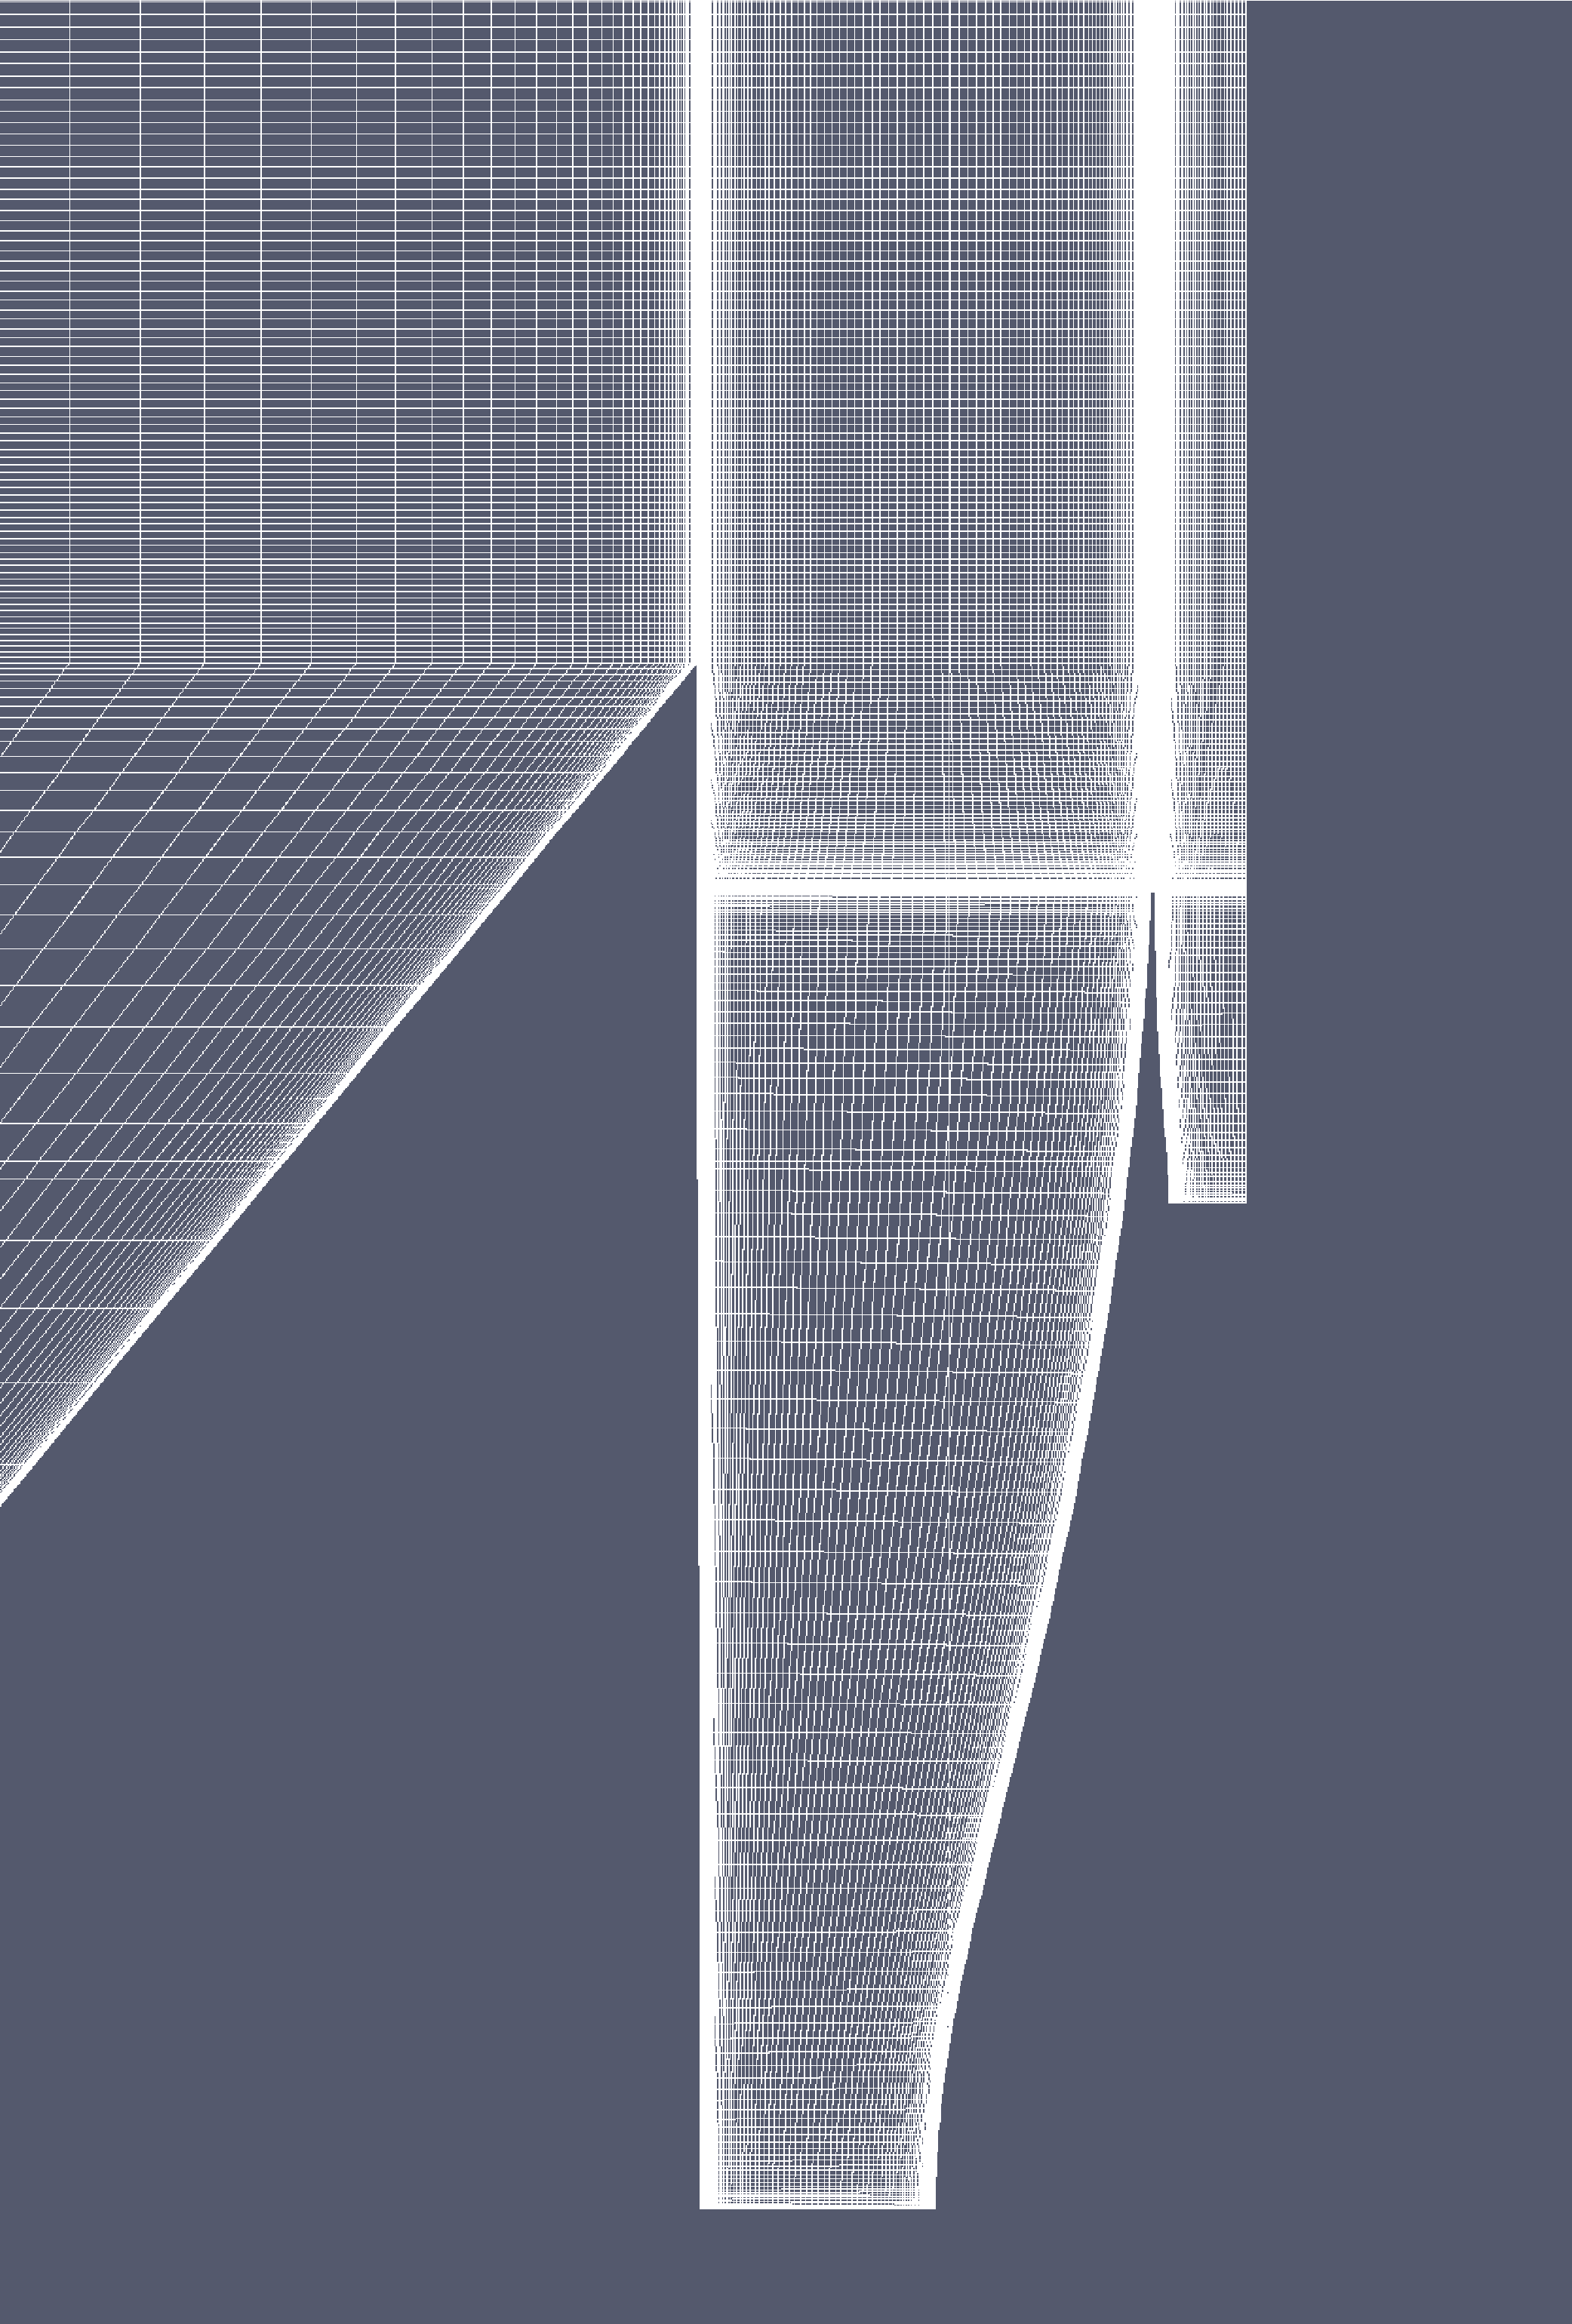
\includegraphics[width=7cm]{./chap5-coaxial-jets/figs/grid2.pdf}
 }
 \caption{(a) Computational mesh. (b) A close-up view of
          the mesh near exit planes of both nozzles.}
 \label{figure-coaxial-jets-grid}
\end{figure}
%
The supersonic inflow boundary condition is the preferred choice 
of inflow boundary condition for Eilmer3, rather than the subsonic 
inflow boundary condition. As such, the simulations
were started at the throats of both nozzles. Conditions at the throats
were computed by isentropically compressing the flow given in
Table~\ref{given-conditions-coaxial-jet} to sonic conditions. These inferred
conditions are shown in Table~\ref{inferred-conditions-coaxial-jet}.
%
\begin{table}[h]
  \caption{Conditions at throats of both nozzles}
  \label{inferred-conditions-coaxial-jet}
  \begin{center}
    \begin{tabular}{cccl}
      \hline\hline
      Parameter & Value   & Units \\
      \hline
      $P_{coflow,throat}$     & 306.4   & kPa \\
      $T_{coflow,throat}$     & 200.0   & K   \\
      $u_{coflow,throat}$     & 317.0   & m/s \\
      $P_{centrejet,throat}$  & 313.3   & kPa \\
      $T_{centrejet,throat}$  & 236.5   & K   \\
      $u_{centrejet,throat}$  & 759.8   & m/s \\
      \hline \hline
    \end{tabular}
  \end{center}
\end{table}
%
The turbulence intensity and turbulent-to-laminar viscosity ratio were adjusted
such that the $\sqrt{\frac{2}{3}k}$ value from the numerical simulations matched
the experimentally measured rms velocity fluctuations $\sqrt{u^{'2}}$ at the exit plane of
the nozzles (see Figure~\ref{figure-coaxial-jets-nozzle-exit-plane-d}). As described
earlier in Section~\ref{backward-facing-step-results}, a comparison between these 
values should only be treated to be approximate. The turbulence intensity used in 
this simulation was 3.5\% for the coflow jet and 2\% for the centrejet, while the 
turbulent-to-laminar viscosity ratio was 5000 for both jets. All gases used for 
this simulation were assumed to be ideal gases. In addition, a modification to 
Fick's first law of diffusion to allow for turbulent diffusion was used. The 
turbulent Prandtl number was assumed to be 0.75, as recommended in Cutler's paper.


%\subsection{Grid convergence}
%\label{}
%


\subsection{Results \& discussion}
%\label{}
%
A typical schlieren image (with vertical knife edge) from the
experiments of Cutler et. al. \cite{Cutler2006} is shown in Figure~\ref{figure-coaxial-jets-mach-contours-a},
while a contour plot of Mach number from Eilmer3 simulations is
shown in Figure~\ref{figure-coaxial-jets-mach-contours-b}.
Shock and expansion waves enamating from the 0.25-mm-thick centre
body lip (at $x$ = 0\,m) into the coflowing jet can be seen in both 
experimental and numerical visualisations. Similar waves that
propagate into the centre jet in the numerical results are not 
visible in the schlieren image. It is thought that this can be
due to the low refractive index in that region \cite{Cutler2006}.
The overall qualitative agreement between the experimental
and numerical visualisations is good.  
\begin{figure}[h]
 \centering
 \subfigure[]{
   \label{figure-coaxial-jets-mach-contours-a}
%   \fbox{Contents of first subfigure}
   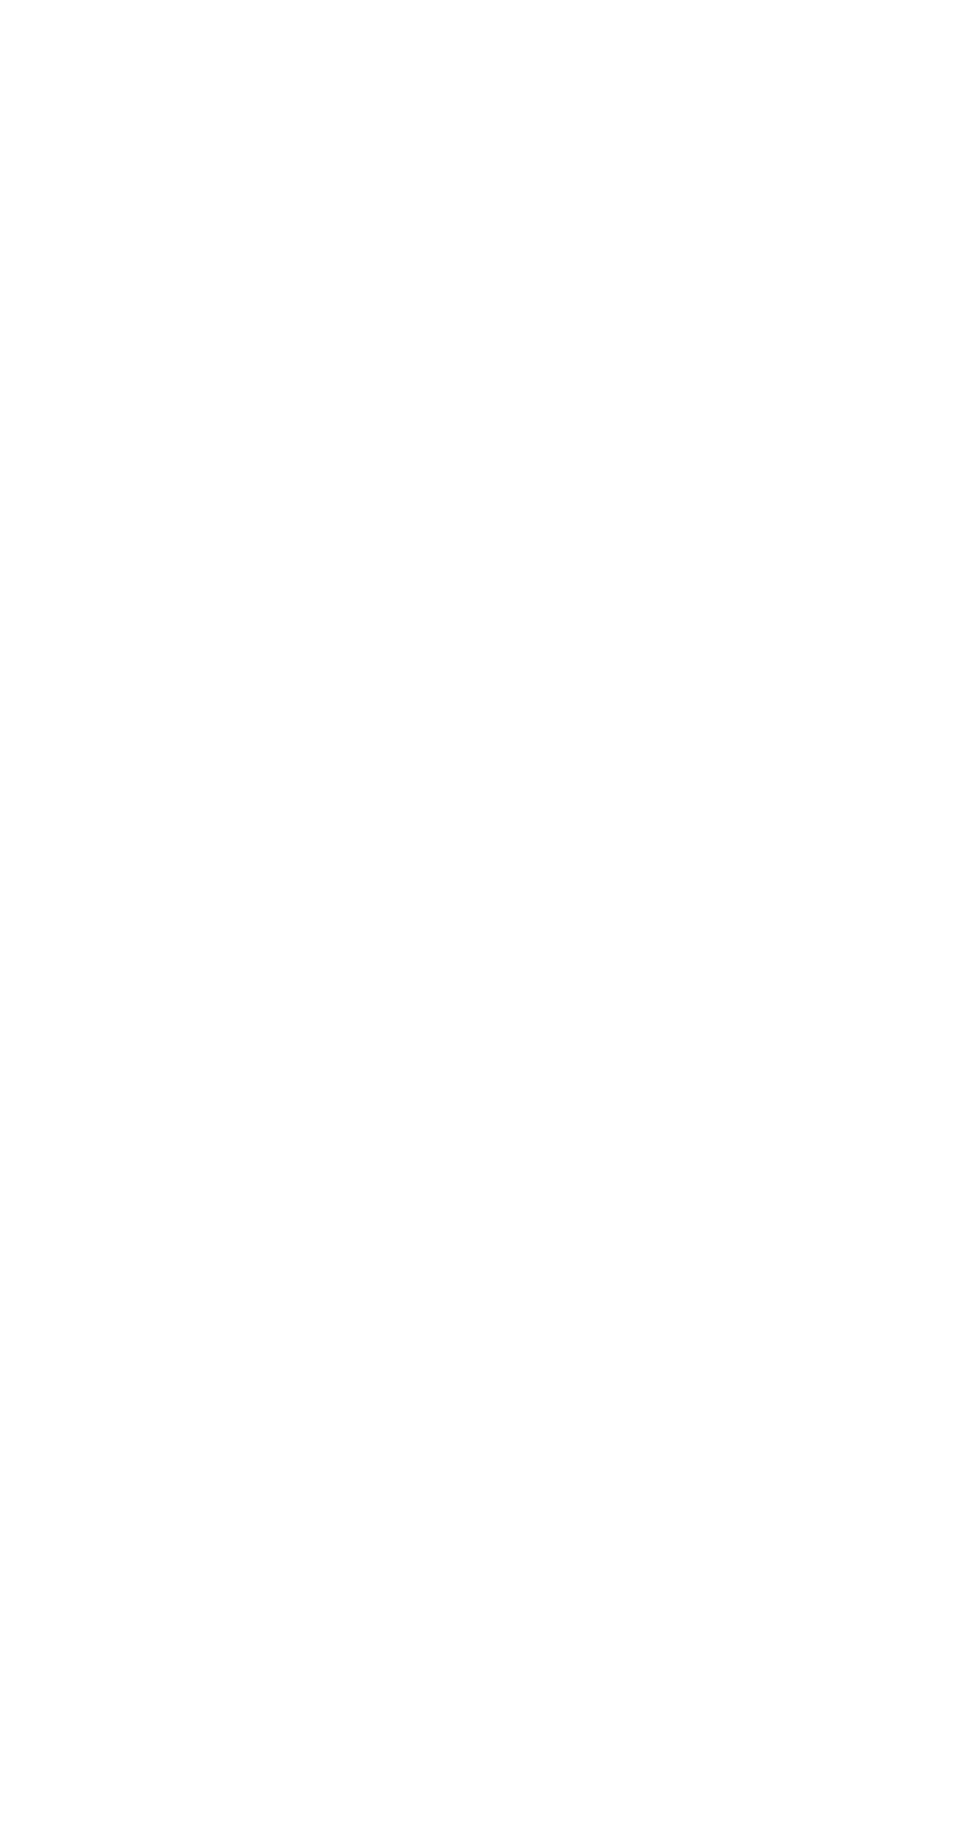
\includegraphics[width=6.5cm]{./chap5-coaxial-jets/figs/coaxial-schlieren-exp.pdf}
 }
 \subfigure[]{
   \label{figure-coaxial-jets-mach-contours-b}
%   \fbox{Contents of second subfigure}
 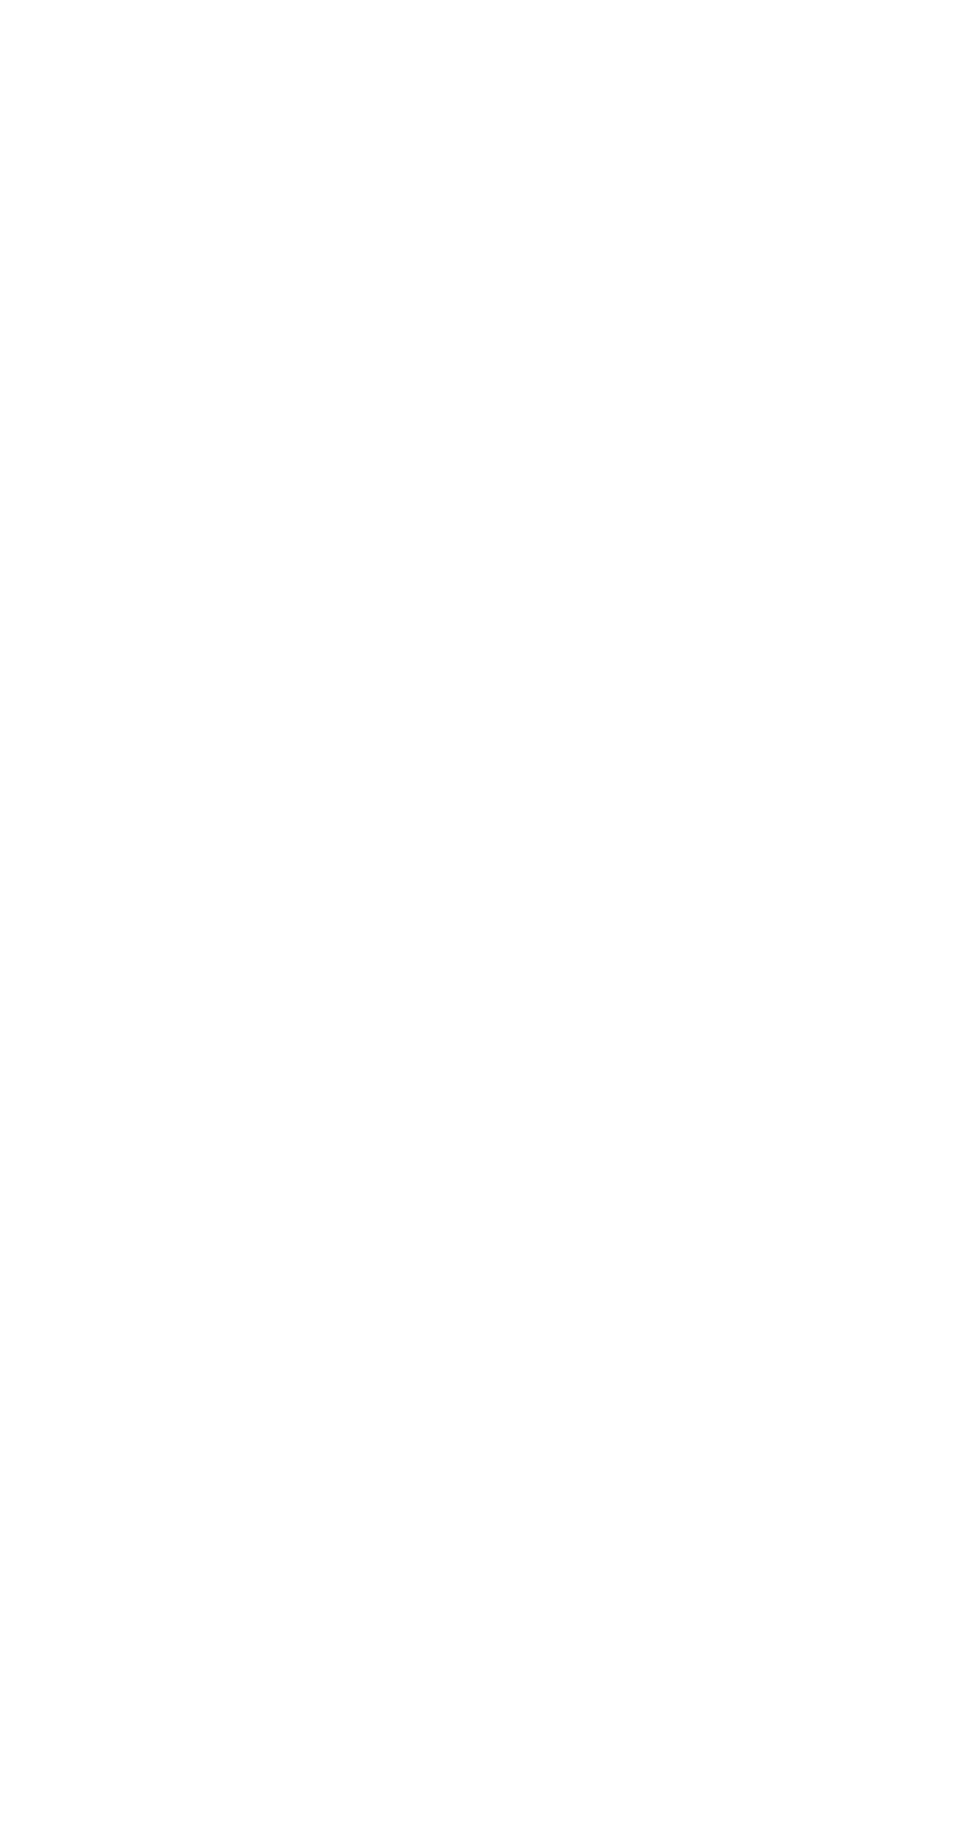
\includegraphics[width=6.5cm]{./chap5-coaxial-jets/figs/coaxial-schlieren-num.pdf}
 }
 \caption{Comparison between (a) experimental schlieren image and 
          (b) numerical Mach number contours}
 \label{figure-coaxial-jets-mach-contours}
\end{figure}

Figure~\ref{figure-coaxial-jets-nozzle-exit-plane} shows the comparison between
experimental data and Eilmer3 simulation results at the first 
measurement plane just downstream of the nozzles exit. The agreement
between experimental data and simulation results is excellent. This agreement 
ensures that the assumptions made for the nozzles in the simulation are valid. 
The agreement is also crucial in showing that the outflow of both jets from 
the nozzles in the experiments are accurately modelled by the Eilmer3 simulations.

Figures~\ref{figure-coaxial-jets-He-O2-mole-fractions-a} and
\ref{figure-coaxial-jets-He-O2-mole-fractions-b} show the comparison
between experimental and simulated He-O$_2$ mole fractions profiles. The 
match between the experimental and simulated He-O$_2$ mole fractions
profiles is excellent until $x$ = 0.22\,m. Downstream of $x$ = 0.22\,m,
the mixing appears to be overpredicted by Eilmer3, hence resulting in a lower
He-O$_2$ mole fraction near the axis of the coaxial jets. Note that at
$x$ = 0.12\,m, there is a sharp discontinuity occurring in Cutler's CFD
results at $y$ = 0.008\,m. This is not evident in the Eilmer3 results.
The better agreement in the Eilmer3 results with the experiments is brought
about by the use of a freestream turbulence intensity that matches that at 
the nozzle exit plane (see Figure~\ref{figure-coaxial-jets-nozzle-exit-plane-d}).

Figure~\ref{figure-coaxial-jets-pitot-pressure-a} and 
\ref{figure-coaxial-jets-pitot-pressure-b} show the comparison
between experimental and simulated pitot pressure profiles. Similar to
the comparison of He-O$_2$ mole fractions, the numerical simulations
agree with the experimental results until about $x$ = 0.22\,m, where the
numerical simulations overpredict the pitot pressure near the axis of
both jets. Also, the matching of the freestream turbulence intensities
at the nozzle exit plane appear to produce a better agreement 
between the numerical simulations and experiments (compare Cutler's CFD
results and Eilmer3 results with the experimental data in Figure~\ref{figure-coaxial-jets-pitot-pressure-b-b}
at $y$ = 0.008\,m). However, both numerical simulations fail to reproduce
the mixing between the coflowing jet and the ambient air (see the sharp
corners in the numerical results at $y$ = 0.023\,m in Figure~\ref{figure-coaxial-jets-pitot-pressure-b-f}).

Figures~\ref{figure-coaxial-jets-u-velocity-a} and 
\ref{figure-coaxial-jets-u-velocity-b} show the comparison
between experimental and simulated  $u$-velocity profiles.
The overall agreement between the numerical and experimental $u$-velocity profiles
is reasonably good, with the exception to two discrepancies. Firstly, 
Eilmer3 does not correctly predict the $u$-velocity profiles in the mixing 
region formed by both jets (see Figure~\ref{figure-coaxial-jets-u-velocity-a}). 
Secondly, the drop in velocity below the nozzle-exit value near the axis 
of both jets is predicted to occur after $x$ = 0.153\,m while it occurs 
experimentally after $x$ = 0.102\,m. 

Figures~\ref{figure-coaxial-jets-rms-velocity-fluctuations-a} and
\ref{figure-coaxial-jets-rms-velocity-fluctuations-b} show the comparison
between experimentally measured rms velocity fluctuations $\sqrt{u^{'2}}$ 
and the numerically derived $\sqrt{\frac{2}{3}k}$. As mentioned earlier, the
comparison between these two quantities is valid only in truly isotropic
turbulent flows. As such, this comparison should only be treated to be
an approximate one. It can be seen in all plots that the experimentally measured
rms fluctuation levels in the coflow jet increases downstream of the exit of the 
nozzle. In contrast, Eilmer3 predicts that these levels remain constant in the 
coflow jet. Apart from this difference, the computed peak amplitudes are roughly 
consistent with the experimental data.

This validation exercise shows that Eilmer3 can be used to predict the development 
of the turbulent mixing in coaxial jets. This validation also shows that matching
the turbulence intensities to those measured experimentally at the inflow plane
aids in getting a more accurate numerical prediction of the downstream flow
development.


\begin{figure}[h]
 \centering
 \subfigure[]{
   \label{figure-coaxial-jets-nozzle-exit-plane-a}
%   \fbox{Contents of first subfigure}
   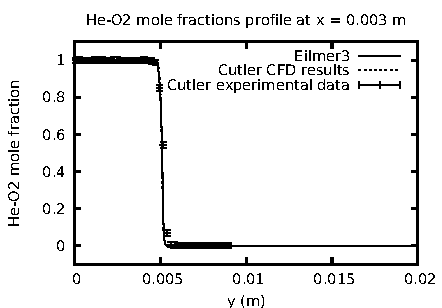
\includegraphics[width=7.5cm]{./chap5-coaxial-jets/figs/He-O2-Mole-Fractions-2D-x003.pdf}
 }
 \subfigure[]{
   \label{figure-coaxial-jets-nozzle-exit-plane-b}
%   \fbox{Contents of second subfigure}
 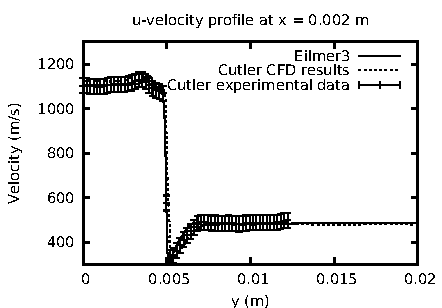
\includegraphics[width=7.5cm]{./chap5-coaxial-jets/figs/u-velocity-2D-x002.pdf}
 }
 \subfigure[]{
   \label{figure-coaxial-jets-nozzle-exit-plane-c}
%   \fbox{Contents of first subfigure}
   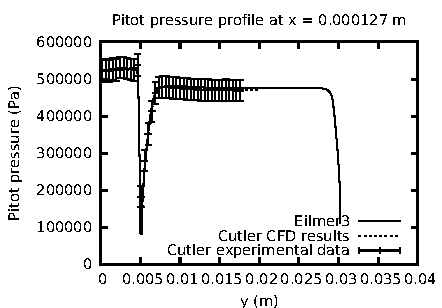
\includegraphics[width=7.5cm]{./chap5-coaxial-jets/figs/Pitot-pressure-2D-x000127.pdf}
 }
 \subfigure[]{
   \label{figure-coaxial-jets-nozzle-exit-plane-d}
%   \fbox{Contents of second subfigure}
 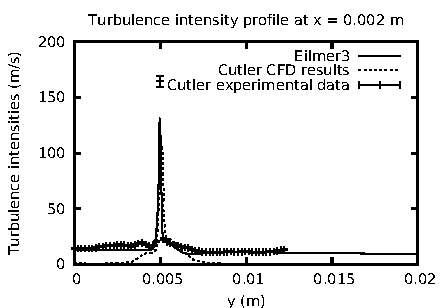
\includegraphics[width=7.5cm]{./chap5-coaxial-jets/figs/rms-velocity-fluctuations-2D-x002.pdf}
 }
 \caption{Comparison of flow variables at nozzle exit plane}
 \label{figure-coaxial-jets-nozzle-exit-plane}
\end{figure}

\begin{figure}[h]
 \centering
 \subfigure[]{
   \label{}
%   \fbox{Contents of first subfigure}
   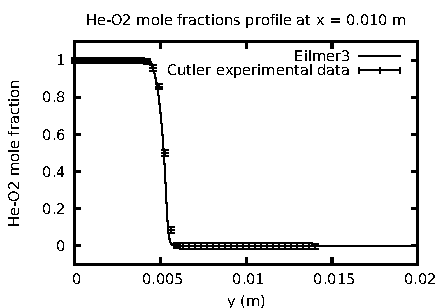
\includegraphics[width=7.5cm]{./chap5-coaxial-jets/figs/He-O2-Mole-Fractions-2D-x010.pdf}
 }
 \subfigure[]{
   \label{}
%   \fbox{Contents of second subfigure}
 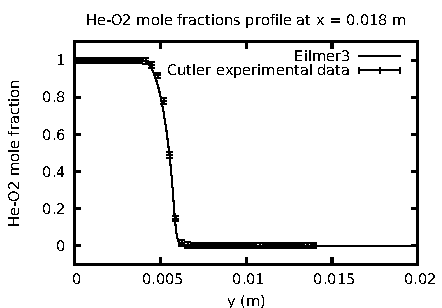
\includegraphics[width=7.5cm]{./chap5-coaxial-jets/figs/He-O2-Mole-Fractions-2D-x018.pdf}
 }
 \subfigure[]{
   \label{}
%   \fbox{Contents of first subfigure}
   \includegraphics[width=7.5cm]{./chap5-coaxial-jets/figs/He-O2-Mole-Fractions-2D-x028.pdf}
 }
 \subfigure[]{
   \label{}
%   \fbox{Contents of second subfigure}
 \includegraphics[width=7.5cm]{./chap5-coaxial-jets/figs/He-O2-Mole-Fractions-2D-x043.pdf}
 }
 \subfigure[]{
   \label{}
%   \fbox{Contents of first subfigure}
   \includegraphics[width=7.5cm]{./chap5-coaxial-jets/figs/He-O2-Mole-Fractions-2D-x062.pdf}
 }
 \subfigure[]{
   \label{}
%   \fbox{Contents of second subfigure}
 \includegraphics[width=7.5cm]{./chap5-coaxial-jets/figs/He-O2-Mole-Fractions-2D-x081.pdf}
 }
 \caption{He-O$_2$ mole fractions from $x$ = 0.01\,m to $x$ = 0.08\,m}
 \label{figure-coaxial-jets-He-O2-mole-fractions-a}
\end{figure}
%
\begin{figure}[h]
 \centering
 \subfigure[]{
   \label{}
%   \fbox{Contents of first subfigure}
   \includegraphics[width=7.5cm]{./chap5-coaxial-jets/figs/He-O2-Mole-Fractions-2D-x101.pdf}
 }
 \subfigure[]{
   \label{}
%   \fbox{Contents of second subfigure}
 \includegraphics[width=7.5cm]{./chap5-coaxial-jets/figs/He-O2-Mole-Fractions-2D-x121.pdf}
 }
 \subfigure[]{
   \label{}
%   \fbox{Contents of first subfigure}
   \includegraphics[width=7.5cm]{./chap5-coaxial-jets/figs/He-O2-Mole-Fractions-2D-x151.pdf}
 }
 \subfigure[]{
   \label{}
%   \fbox{Contents of second subfigure}
 \includegraphics[width=7.5cm]{./chap5-coaxial-jets/figs/He-O2-Mole-Fractions-2D-x181.pdf}
 }
 \subfigure[]{
   \label{}
%   \fbox{Contents of first subfigure}
   \includegraphics[width=7.5cm]{./chap5-coaxial-jets/figs/He-O2-Mole-Fractions-2D-x220.pdf}
 }
 \subfigure[]{
   \label{}
%   \fbox{Contents of second subfigure}
 \includegraphics[width=7.5cm]{./chap5-coaxial-jets/figs/He-O2-Mole-Fractions-2D-x261.pdf}
 }
 \caption{He-O$_2$ mole fractions from $x$ = 0.10\,m to $x$ = 0.26\,m}
 \label{figure-coaxial-jets-He-O2-mole-fractions-b}
\end{figure}

\begin{figure}[h]
 \centering
 \subfigure[]{
   \label{}
%   \fbox{Contents of first subfigure}
   \includegraphics[width=7.5cm]{./chap5-coaxial-jets/figs/Pitot-pressure-2D-x003.pdf}
 }
 \subfigure[]{
   \label{}
%   \fbox{Contents of second subfigure}
 \includegraphics[width=7.5cm]{./chap5-coaxial-jets/figs/Pitot-pressure-2D-x010.pdf}
 }
 \subfigure[]{
   \label{}
%   \fbox{Contents of first subfigure}
   \includegraphics[width=7.5cm]{./chap5-coaxial-jets/figs/Pitot-pressure-2D-x028.pdf}
 }
 \subfigure[]{
   \label{}
%   \fbox{Contents of second subfigure}
 \includegraphics[width=7.5cm]{./chap5-coaxial-jets/figs/Pitot-pressure-2D-x043.pdf}
 }
 \subfigure[]{
   \label{}
%   \fbox{Contents of first subfigure}
   \includegraphics[width=7.5cm]{./chap5-coaxial-jets/figs/Pitot-pressure-2D-x062.pdf}
 }
 \subfigure[]{
   \label{}
%   \fbox{Contents of second subfigure}
 \includegraphics[width=7.5cm]{./chap5-coaxial-jets/figs/Pitot-pressure-2D-x081.pdf}
 }
 \caption{Pitot pressure from $x$ = 0.003\,m to $x$ = 0.08\,m}
 \label{figure-coaxial-jets-pitot-pressure-a}
\end{figure}
%
\begin{figure}[h]
 \centering
 \subfigure[]{
   \label{}
%   \fbox{Contents of first subfigure}
   \includegraphics[width=7.5cm]{./chap5-coaxial-jets/figs/Pitot-pressure-2D-x101.pdf}
 }
 \subfigure[]{
   \label{figure-coaxial-jets-pitot-pressure-b-b}
%   \fbox{Contents of second subfigure}
 \includegraphics[width=7.5cm]{./chap5-coaxial-jets/figs/Pitot-pressure-2D-x121.pdf}
 }
 \subfigure[]{
   \label{}
%   \fbox{Contents of first subfigure}
   \includegraphics[width=7.5cm]{./chap5-coaxial-jets/figs/Pitot-pressure-2D-x151.pdf}
 }
 \subfigure[]{
   \label{}
%   \fbox{Contents of second subfigure}
 \includegraphics[width=7.5cm]{./chap5-coaxial-jets/figs/Pitot-pressure-2D-x181.pdf}
 }
 \subfigure[]{
   \label{}
%   \fbox{Contents of first subfigure}
   \includegraphics[width=7.5cm]{./chap5-coaxial-jets/figs/Pitot-pressure-2D-x220.pdf}
 }
 \subfigure[]{
   \label{figure-coaxial-jets-pitot-pressure-b-f}
%   \fbox{Contents of second subfigure}
 \includegraphics[width=7.5cm]{./chap5-coaxial-jets/figs/Pitot-pressure-2D-x261.pdf}
 }
 \caption{Pitot pressure from $x$ = 0.10\,m to $x$ = 0.26\,m}
 \label{figure-coaxial-jets-pitot-pressure-b}
\end{figure}

\begin{figure}[h]
 \centering
 \subfigure[]{
   \label{}
%   \fbox{Contents of first subfigure}
   \includegraphics[width=7.5cm]{./chap5-coaxial-jets/figs/u-velocity-2D-x005.pdf}
 }
 \subfigure[]{
   \label{}
%   \fbox{Contents of second subfigure}
 \includegraphics[width=7.5cm]{./chap5-coaxial-jets/figs/u-velocity-2D-x012.pdf}
 }
 \subfigure[]{
   \label{}
%   \fbox{Contents of first subfigure}
   \includegraphics[width=7.5cm]{./chap5-coaxial-jets/figs/u-velocity-2D-x027.pdf}
 }
 \subfigure[]{
   \label{}
%   \fbox{Contents of second subfigure}
 \includegraphics[width=7.5cm]{./chap5-coaxial-jets/figs/u-velocity-2D-x042.pdf}
 }
 \subfigure[]{
   \label{}
%   \fbox{Contents of first subfigure}
   \includegraphics[width=7.5cm]{./chap5-coaxial-jets/figs/u-velocity-2D-x062.pdf}
 }
 \subfigure[]{
   \label{}
%   \fbox{Contents of second subfigure}
 \includegraphics[width=7.5cm]{./chap5-coaxial-jets/figs/u-velocity-2D-x082.pdf}
 }
 \caption{$u$-velocity from $x$ = 0.005\,m to $x$ = 0.08\,m}
 \label{figure-coaxial-jets-u-velocity-a}
\end{figure}
%
\begin{figure}[h]
 \centering
 \subfigure[]{
   \label{}
%   \fbox{Contents of first subfigure}
   \includegraphics[width=7.5cm]{./chap5-coaxial-jets/figs/u-velocity-2D-x102.pdf}
 }
 \subfigure[]{
   \label{}
%   \fbox{Contents of second subfigure}
 \includegraphics[width=7.5cm]{./chap5-coaxial-jets/figs/u-velocity-2D-x123.pdf}
 }
 \subfigure[]{
   \label{}
%   \fbox{Contents of first subfigure}
   \includegraphics[width=7.5cm]{./chap5-coaxial-jets/figs/u-velocity-2D-x153.pdf}
 }
 \subfigure[]{
   \label{}
%   \fbox{Contents of second subfigure}
 \includegraphics[width=7.5cm]{./chap5-coaxial-jets/figs/u-velocity-2D-x190.pdf}
 }
 \subfigure[]{
   \label{}
%   \fbox{Contents of first subfigure}
   \includegraphics[width=7.5cm]{./chap5-coaxial-jets/figs/u-velocity-2D-x220.pdf}
 }
 \subfigure[]{
   \label{}
%   \fbox{Contents of second subfigure}
 \includegraphics[width=7.5cm]{./chap5-coaxial-jets/figs/u-velocity-2D-x258.pdf}
 }
 \caption{$u$-velocity from $x$ = 0.10\,m to $x$ = 0.26\,m}
 \label{figure-coaxial-jets-u-velocity-b}
\end{figure}

\begin{figure}[h]
 \centering
 \subfigure[]{
   \label{}
%   \fbox{Contents of first subfigure}
   \includegraphics[width=7.5cm]{./chap5-coaxial-jets/figs/rms-velocity-fluctuations-2D-x005.pdf}
 }
 \subfigure[]{
   \label{}
%   \fbox{Contents of second subfigure}
 \includegraphics[width=7.5cm]{./chap5-coaxial-jets/figs/rms-velocity-fluctuations-2D-x012.pdf}
 }
 \subfigure[]{
   \label{}
%   \fbox{Contents of first subfigure}
   \includegraphics[width=7.5cm]{./chap5-coaxial-jets/figs/rms-velocity-fluctuations-2D-x027.pdf}
 }
 \subfigure[]{
   \label{}
%   \fbox{Contents of second subfigure}
 \includegraphics[width=7.5cm]{./chap5-coaxial-jets/figs/rms-velocity-fluctuations-2D-x042.pdf}
 }
 \subfigure[]{
   \label{}
%   \fbox{Contents of first subfigure}
   \includegraphics[width=7.5cm]{./chap5-coaxial-jets/figs/rms-velocity-fluctuations-2D-x062.pdf}
 }
 \subfigure[]{
   \label{}
%   \fbox{Contents of second subfigure}
 \includegraphics[width=7.5cm]{./chap5-coaxial-jets/figs/rms-velocity-fluctuations-2D-x082.pdf}
 }
 \caption{Turbulence intensities from $x$ = 0.005\,m to $x$ = 0.08\,m}
 \label{figure-coaxial-jets-rms-velocity-fluctuations-a}
\end{figure}
%
\begin{figure}[h]
 \centering
 \subfigure[]{
   \label{}
%   \fbox{Contents of first subfigure}
   \includegraphics[width=7.5cm]{./chap5-coaxial-jets/figs/rms-velocity-fluctuations-2D-x102.pdf}
 }
 \subfigure[]{
   \label{}
%   \fbox{Contents of second subfigure}
 \includegraphics[width=7.5cm]{./chap5-coaxial-jets/figs/rms-velocity-fluctuations-2D-x123.pdf}
 }
 \subfigure[]{
   \label{}
%   \fbox{Contents of first subfigure}
   \includegraphics[width=7.5cm]{./chap5-coaxial-jets/figs/rms-velocity-fluctuations-2D-x153.pdf}
 }
 \subfigure[]{
   \label{}
%   \fbox{Contents of second subfigure}
 \includegraphics[width=7.5cm]{./chap5-coaxial-jets/figs/rms-velocity-fluctuations-2D-x190.pdf}
 }
 \subfigure[]{
   \label{}
%   \fbox{Contents of first subfigure}
   \includegraphics[width=7.5cm]{./chap5-coaxial-jets/figs/rms-velocity-fluctuations-2D-x220.pdf}
 }
 \subfigure[]{
   \label{}
%   \fbox{Contents of second subfigure}
 \includegraphics[width=7.5cm]{./chap5-coaxial-jets/figs/rms-velocity-fluctuations-2D-x258.pdf}
 }
 \caption{Turbulence intensities from $x$ = 0.10\,m to $x$ = 0.26\,m}
 \label{figure-coaxial-jets-rms-velocity-fluctuations-b}
\end{figure}


% 3D examples
\newpage
\section{Three-dimensional flat plate}
\label{chapter-3Dflatplate}
%
This test case is a 3D extension of a previous 2D test case, featuring Mach 4.5 air flow across a two-dimensional flat plate. The original 2D flat plate test case is an example included in the Eilmer3 CFD suite to demonstrate the $k$-$\omega$ turbulence model. 

The example includes experimentally validated flow data extracted at $x=0.368$\,m from Mabey's 7402 series test case (documented by Fernholz and Finley~\cite{Fernholz1977}), skin friction coefficient data by Van Driest~\cite{vanDriest1956}, as well as post-processed and graphed results for the original 2D simulation. This provides sufficient information for comparison and validation of the three-dimensional extended case. 
%------------------------------------------------------------------
\subsection{Details of flow problem}
%\label{}
Figure~\ref{f:tc1:scheme} indicates the basic schematic for the flat plate flow. For the original 2D simulation, the fluid domain was specified as a single $x$-$y$ slice with a length ($x$) of $0.4$\,m. 
%
\begin{figure}[htbp]
 \begin{center}
  \includegraphics[width=9cm]{./chap6-3Dflatplate/figs/schematic2.pdf}
  \caption{Basic Schematic for Flat Plate Simulations.}
  \label{f:tc1:scheme}
 \end{center}
\end{figure}
%
A segment of fluid around the plate was selected using a new co-ordinate system, as indicated in Figure~\ref{f:tc1:fluid}, and inverted, resulting in the flat plate edge shifting to the top of the fluid domain. The wedged shape was used to allow viscous effects at the plate's leading edge to be properly realised, by providing sufficient space for any shocks or boundary layers to form without errors due to the domain size. 
%
\begin{figure}[htbp]
 \begin{center}
  \includegraphics[width=12cm]{./chap6-3Dflatplate/figs/fluidvolume.pdf}
  \caption{Fluid Domain for 2D Flat Plate Simulation (not to scale).}
  \label{f:tc1:fluid}
 \end{center}
\end{figure}
%

For the 3D case, the selected domain was extended in the $Y$ direction by $0.01$\,m to capture flow along a strip of the plate. All other dimensions were kept identical in order to allow proper replication of the 2D results. The flow properties from the 2D flat plate, including pressure, velocity, temperature and density, were utilised by the 3D flat plate case as initial and inflow conditions (Table~\ref{t:tc1:initial}) in an attempt to ensure the results from both cases were identical.
%
\begin{table}[htbp]
  \caption{3D Flat Plate Initial \& Inflow (Freestream) Conditions.}
  \label{t:tc1:initial}
  \begin{center}
  \begin{tabular}{cccl}
  \hline\hline
     Parameter  & Value & Units \\
  \hline
    $P_\infty$  & $3.160$ & kPa  \\
    $U_\infty$  & $712.9$ & m/s  \\
    $T_\infty$  & $62.16$ & K  \\
    $\rho_\infty$  & $0.177$ & kg/m$^3$  \\
  \hline\hline
  \end{tabular}
  \end{center}
\end{table}

%
The turbulence variables $k$ and $\omega$ were initialised using a turbulence intensity of $1\%$ and turbulent-to-laminar viscosity ratio of $1$, as in the 2D flat plate case. Table~\ref{t:tc1:turb} indicates the estimated turbulence quantities used by the 3D flat plate as initial conditions.
%
\begin{table}[htbp]
  \caption{3D Flat Plate Initial (Freestream) Turbulence Properties.}
  \label{t:tc1:turb}
  \begin{center}
  \begin{tabular}{cccl}
  \hline\hline
     Parameter  & Value & Units \\
  \hline
    Turbulence Kinetic Energy ($k$)  & $76.23$ & m$^2$/s$^2$  \\
    Specific Dissipation Rate ($\omega$)  & $32.65\times10^5$ & /s  \\
  \hline\hline
  \end{tabular}
  \end{center}
\end{table}
%

\subsection{Details of computational approach}
%\label{}
The fluid domain geometry from the 2D test case of $0.4$\,m$\times0.16$\,m (with the leading edge side raised $0.12$\,m) was altered to include the 3D extension of $0.01$\,m. The co-ordinates and representative control volume were utilised in the Eilmer3 simulation, as indicated in Figure~\ref{f:tc1:geometry}.
%
\begin{figure}[htbp]
 \begin{center}
  \includegraphics[width=12cm]{./chap6-3Dflatplate/figs/3Dcoordinates.pdf}
  \caption{3D Flat Plate Mesh Geometry (not to scale).}
  \label{f:tc1:geometry}
 \end{center}
\end{figure}
%
Following the 2D Flat Plate example, the geometry was divided into a $128\times96$ grid extended into 3D by 10 cells, resulting in an overall grid resolution of $128\times96\times10$ (122880) cells (Figure~\ref{f:tc1:mesh}). 
The top face of the fluid domain was represented as an adiabatic wall, the west and bottom faces as supersonic inflow, and the east face as supersonic outflow as indicated in Figures~\ref{f:tc1:fluid} and~\ref{f:tc1:geometry}. Both the north and south boundaries were set as slip walls to ensure no interference with the fluid flow, and allow the 2D results to be representative of a 'slice' of the 3D solution due to uniformity along the domain width.
%
\begin{figure}[htbp]
 \begin{center}
  \includegraphics[width=12cm]{./chap6-3Dflatplate/figs/tc1meshbw.png}
  \caption{3D Flat Plate Simulation Mesh.}
  \label{f:tc1:mesh}
 \end{center}
\end{figure}
%
As per the 2D test case, clustering towards the leading edge and flat plate was utilised in order to ensure the $y^+<1$ criteria was met, to accurately simulate turbulence (Figure~\ref{f:tc1:mesh}). Clustering along the $Y$ direction in the 3D case was not necessary, as the north and south surfaces do not experience viscous effects.

In order to minimise simulation time, the fluid domain was split into sixteen individual blocks, to be solved separately using sixteen simultaneous threads of the Eilmer3 solver. The main block was divided into four sub-blocks along the $X$ axis and two sub-blocks along the $Y$ and $Z$ axes ($4\times2\times2$). Due to the clustering in the $X$ and $Z$ directions towards the leading edge and surface of the flat plate, the sub-blocks were differently sized in the $X$ and $Z$ directions, but equally spaced in the $Y$ direction.

\subsection{Grid convergence}
%\label{}
A grid convergence study was completed using the full resolution and a $20\%$ reduced version ($100\times8\times76$). An investigation into skin friction coefficient ($C_f$) between the two versions indicated a maximum divergence of $5\%$ during the leading edge peaks, and an average difference of $<1\%$ (Figures~\ref{f:tc1:res} and~\ref{f:tc1:comp}). Mach number, pressure, temperature and velocity comparisons did not indicate convergence (Figure~\ref{f:tc1:convergence}), as the difference in boundary layer thickness shows the effect grid resolution has on turbulent transition. The full resolution was concluded to be sufficient, as the goal of Test Case 1 was to replicate another simulation's results, not refine them. 
%
\begin{figure}[h]
 \begin{center}
  \includegraphics[width=9.2cm]{./chap6-3Dflatplate/figs/tc1-cf-resolution.pdf}
  \caption{3D Flat Plate Grid Convergence - $C_f$ at $x=0.290$\,m.}
  \label{f:tc1:res}
  \vspace{1cm}
  \includegraphics[width=9.2cm]{./chap6-3Dflatplate/figs/gridconverge/tc1-cf-comparison.pdf}
  \caption{3D Flat Plate Grid Convergence - Surface $C_f$.}
  \label{f:tc1:comp}
 \end{center}
\end{figure}
%
\begin{figure}[p]
 \centering
 \subfigure[Mach Number.]{
   \label{}
%   \fbox{Contents of first subfigure}
   \includegraphics[width=7.5cm]{./chap6-3Dflatplate/figs/gridconverge/tc1-mach-comparison.pdf}
 }
 \subfigure[Pitot Pressure.]{
   \label{}
%   \fbox{Contents of second subfigure}
 \includegraphics[width=7.5cm]{./chap6-3Dflatplate/figs/gridconverge/tc1-pitot-comparison.pdf}
 }
 \subfigure[Temperature.]{
   \label{}
%   \fbox{Contents of first subfigure}
   \includegraphics[width=7.5cm]{./chap6-3Dflatplate/figs/gridconverge/tc1-temp-comparison.pdf}
 }
 \subfigure[Velocity.]{
   \label{}
%   \fbox{Contents of second subfigure}
 \includegraphics[width=7.5cm]{./chap6-3Dflatplate/figs/gridconverge/tc1-u-comparison.pdf}
 }
 \caption{3D Flat Plate Grid Convergence - Flow Properties.}
 \label{f:tc1:convergence}
\end{figure}

\clearpage
\subsection{Results \& discussion}
%\label{}
The flow field was tested for $1.68$ milliseconds (approximately three flow lengths), to ensure steady-state conditions were reached. This was achieved via simulation on `Barrine' for $177.78$ hours ($2844.53$ CPU-hours). Paraview was used to view the Mach number (Figure~\ref{f:tc1:mach}) and pressure (Figure~\ref{f:tc1:pressure}) data at steady-state.
%
\begin{figure}[htbp]
 \begin{center}
  \includegraphics[width=16cm]{./chap6-3Dflatplate/figs/testcase1mach2.png}
  \caption{3D Flat Plate Mach Data.}
  \label{f:tc1:mach}
 \end{center}
\end{figure}
%

As indicated in Figure~\ref{f:tc1:mach}, the top edge of the fluid domain has a very low Mach number, due to the presence of the flat plate and turbulent boundary layer. The reduction in velocity associated with the boundary layer is present, which can be observed increasing in thickness along the $X$ axis.
A weak oblique shock, caused by the high speed flow interaction with the leading edge of the flat plate, is indicated as a slight change in velocity parallel to the bottom  boundary.
%
\begin{figure}[htbp]
 \begin{center}
  \includegraphics[width=16cm]{./chap6-3Dflatplate/figs/testcase1pressure2.png}
  \caption{3D Flat Plate Pressure Data.}
  \label{f:tc1:pressure}
 \end{center}
\end{figure}
%
Figure~\ref{f:tc1:pressure} illustrates the pressure difference over the flow domain. As with Mach number, the top surface illustrates a low pressure due to the presence of a turbulent boundary layer. The shock is much more prominent, as an increase in pressure can be observed immediately behind the shock.

Utilising a post-processing script and a modified viscous properties calculator, $X$-$Z$ slices were taken at each cell in the $Y$ direction and plotted together, in order to validate that the extension into 3D did not affect the results.
%
\begin{figure}[htbp]
 \begin{center}
  \includegraphics[width=10cm]{./chap6-3Dflatplate/figs/3Dslices/mabey-cf.pdf}
  \caption{3D Flat Plate Surface $C_f$.}
  \label{f:tc1:cf}
 \end{center}
\end{figure}
%
Skin friction coefficient ($C_f$) was extracted along the flat plate surface ($y=0.16$\,m), while temperature, Mach number, pitot pressure and velocity were extracted from a vertical slice $0.368$\,m from the leading edge, in order to allow a comparison with Mabey's experimental data. Excellent similarity was observed between the slices, as indicated by the $C_f$ data in Figure~\ref{f:tc1:cf} and other properties in Figure~\ref{f:tc1:profiles}. 

Deviation between the slices depended on the cell position, with the largest deviation in $C_f$ (of the order $10^{-4}$) occurring at the peak during boundary layer transition. Mach number, temperature, pitot pressure and velocity featured zero deviation far from the flat-plate surface, but grew as distance to the plate decreased, to the orders of $10^{-4}$, $10^{-1}$\,K, $10^{-1}$\,Pa and $10^{-2}$\,m/s at the surface respectively.
%
\begin{figure} %[htbp]%
	\centering
	\subfigure[][Mach number (M) vs. Height (mm).]{\includegraphics[width=7.5cm]{./chap6-3Dflatplate/figs/3Dslices/mabey-mach.pdf}}%
	\qquad
	\subfigure[][Velocity (m/s) vs. Height (mm).]{\includegraphics[width=7.5cm]{./chap6-3Dflatplate/figs/3Dslices/mabey-u.pdf}}
	
	\subfigure[][Pitot Pressure (kPa) vs. Height (mm).]{\includegraphics[width=7.5cm]{./chap6-3Dflatplate/figs/3Dslices/mabey-pitot.pdf}}%
	\qquad
	\subfigure[][Temperature (K) vs Height (mm).]{\includegraphics[width=7.5cm]{./chap6-3Dflatplate/figs/3Dslices/mabey-temperature.pdf}}
	\caption{3D Flat Plate Boundary Layer Profiles at $x=0.368$\,m.}%
	\label{f:tc1:profiles}%
\end{figure}
%
Once the internal 3D validation was completed, the comparison between the 2D and 3D
flow schemes was undertaken. This comparison was made by graphing the original 2D test case data with a single slice from the 3D flat plate. As shown in Figure~\ref{f:tc1:2Dv3Dprofiles}, the 2D and 3D data for Mach number, temperature, pitot pressure and velocity correlate well at $x=0.368$\,m, while Figure~\ref{f:tc1:2Dv3Dcf} indicates a noticeable difference in skin friction coefficient along the flat-plate between the simulations.
Far-field values for Mach number, temperature, pitot pressure and velocity feature zero deviation between the simulations , but grew to the order of $10^{-3}$, $10^{-1}$\,K, $10^1$\,Pa and $10^{-1}$\,m/s respectively at the flat plate surface. 

By extending the flat plate into three dimensions, velocity had transformed from a 2D vector to a 3D vector. Data analysis indicated that $Y$ velocity components arose in the 3D simulation which were not present in 2D, as well as a reduction in the $X$ and $Z$ velocity components.  The $Y$ velocities in the far-field are of the order of $10^{-9}$\,m/s, however are observed to peak at $10^{-3}$\,m/s close to the flat plate surface and fluctuate between positive and negative values as the distance from the leading edge increases. Due to skin friction coefficient's dependence on parallel ($X$ direction) velocity and temperature, these large deviations observed at the surface are expected to be the cause of the $10^{-4}$ deviation in $C_f$ seen in Figure~\ref{f:tc1:2Dv3Dcf}.
%
\begin{figure}[htbp]
 \begin{center}
  \includegraphics[width=10cm]{./chap6-3Dflatplate/figs/2Dto3D/mabey-cf1.pdf}
  \caption{3D vs 2D Flat Plate Surface $C_f$.}
  \label{f:tc1:2Dv3Dcf}
 \end{center}
\end{figure}
%

While the 2D flat plate results weren't replicated perfectly, extending the case into 3D altered the turbulent flow effects and identified a limitation of the three-dimensional turbulence simulation. It was expected that there would be no $Y$ velocity components due to flow symmetry, as the 2D flat plate extension into 3D represented an ideal `slice'. The observed difference in skin friction coefficient indicated the development of $Y$ velocity components within the turbulent boundary layer, identifying a potential bug in the solver. 
%
\begin{figure} [htbp]
	\centering
	\subfigure[][Mach number (M) vs. Height (mm).]{\includegraphics[width=7.5cm]{./chap6-3Dflatplate/figs/2Dto3D/mabey-mach.pdf}}%
	\qquad
	\subfigure[][Velocity (m/s) vs. Height (mm).]{\includegraphics[width=7.5cm]{./chap6-3Dflatplate/figs/2Dto3D/mabey-u.pdf}}
	
	\subfigure[][Pitot Pressure (kPa) vs. Height (mm).]{\includegraphics[width=7.5cm]{./chap6-3Dflatplate/figs/2Dto3D/mabey-pitot.pdf}}%
	\qquad
	\subfigure[][Temperature (K) vs Height (mm).]{\includegraphics[width=7.5cm]{./chap6-3Dflatplate/figs/2Dto3D/mabey-temperature.pdf}}
	\caption{3D vs 2D Flat Plate Boundary Layer Profiles at $x=0.368$\,m.}%
	\label{f:tc1:2Dv3Dprofiles}%
\end{figure}
\newpage
\section{Three-dimensional single fin}
\label{chapter-3Dsinglefin}
%

%------------------------------------------------------------------
\subsection{Details of flow problem}
%\label{}

\subsection{Details of computational approach}
%\label{}

\subsection{Results \& discussion}
%\label{}
\newpage
\section{Three-dimensional normal injector}
\label{chapter-3Dinjector}
%

%------------------------------------------------------------------
\subsection{Details of flow problem}
%\label{}

\subsection{Details of computational approach}
%\label{}

\subsection{Results \& discussion}
%\label{}

% conclusion.tex

\newpage
\section{Conclusion}
\label{chapter-conclusion}
Wilcox's 2006 $k$-$\omega$ turbulence model has been implemented in 
Eilmer3 and validated against seven test cases (four two-dimensional and three three-dimensional) that had flowfields 
representative of those to be expected in hypersonic airbreathing 
propulsion. 

The first test case showed that Eilmer3 can be used to 
predict turbulent boundary layer profiles 
and skin friction distribution for a Mach 4 flow on a flat plate 
despite the turbulence model's sensitivity to user-defined freestream 
turbulence properties. The second test case, an axisymmetric analogy 
of the flat plate test case, showed that Eilmer3 can be used to 
predict turbulent heat flux distribution on the external surface of a cylinder 
in a Mach 9 flow. This test case also demonstrated that $y^+$ values
and maximum cell aspect ratios should be kept below 1 and 600
respectively for turbulent CFD simulations. The third test case showed
that Eilmer3 can be used to predict the boundary layer profiles of
a Mach 2 flow past a backward facing step and the fourth test case
demonstrated that Eilmer3 can be used to predict the turbulent mixing 
phenomena of two coaxial Mach 2 jets. 
%

The fifth test case was successful in closely replicating the data produced by the two-dimensional flat plate case it extended. Adding a third-dimension resulted in the development of $Y$ velocity components between the cells, and a lowered parallel ($X$ direction) velocity within the turbulent boundary layer for the $C_f$ calculations. The differences in skin friction coefficient $C_f$, but close correlation with other flow properties, helped to identify a potential bug in the solver caused by extending the case into 3D. 

%--------------------------------------------------------------------

\newpage
\bibliographystyle{unsrt}
%\bibliography{bibtex/pj,bibtex/computing,bibtex/gas_dynamic,bibtex/adm}
\bibliography{./bibliography/phd_bibliography}
%\bibliographystyle{newapa}

\newpage
\appendix

\end{document}
